
%% bare_jrnl.tex
%% V1.3
%% 2007/01/11
%% by Michael Shell
%% see http://www.michaelshell.org/
%% for current contact information.
%%
%% This is a skeleton file demonstrating the use of IEEEtran.cls
%% (requires IEEEtran.cls version 1.7 or later) with an IEEE journal paper.
%%
%% Support sites:
%% http://www.michaelshell.org/tex/ieeetran/
%% http://www.ctan.org/tex-archive/macros/latex/contrib/IEEEtran/
%% and
%% http://www.ieee.org/

% *** Authors should verify (and, if needed, correct) their LaTeX system  ***
% *** with the testflow diagnostic prior to trusting their LaTeX platform ***
% *** with production work. IEEE's font choices can trigger bugs that do  ***
% *** not appear when using other class files.                            ***
% The testflow support page is at:
% http://www.michaelshell.org/te x/testflow/


%%*************************************************************************
%% Legal Notice:
%% This code is offered as-is without any warranty either expressed or
%% implied; without even the implied warranty of MERCHANTABILITY or
%% FITNESS FOR A PARTICULAR PURPOSE! 
%% User assumes all risk.
%% In no event shall IEEE or any contributor to this code be liable for
%% any damages or losses, including, but not limited to, incidental,
%% consequential, or any other damages, resulting from the use or misuse
%% of any information contained here.
%%
%% All comments are the opinions of their respective authors and are not
%% necessarily endorsed by the IEEE.
%%
%% This work is distributed under the LaTeX Project Public License (LPPL)
%% ( http://www.latex-project.org/ ) version 1.3, and may be freely used,
%% distributed and modified. A copy of the LPPL, version 1.3, is included
%% in the base LaTeX documentation of all distributions of LaTeX released
%% 2003/12/01 or later.
%% Retain all contribution notices and credits.
%% ** Modified files should be clearly indicated as such, including  **
%% ** renaming them and changing author support contact information. **
%%
%% File list of work: IEEEtran.cls, IEEEtran_HOWTO.pdf, bare_adv.tex,
%%                    bare_conf.tex, bare_jrnl.tex, bare_jrnl_compsoc.tex
%%*************************************************************************

% Note that the a4paper option is mainly intended so that authors in
% countries using A4 can easily print to A4 and see how their papers will
% look in print - the typesetting of the document will not typically be
% affected with changes in paper size (but the bottom and side margins will).
% Use the testflow package mentioned above to verify correct handling of
% both paper sizes by the user's LaTeX system.
%
% Also note that the "draftcls" or "draftclsnofoot", not "draft", option
% should be used if it is desired that the figures are to be displayed in
% draft mode.
%
\documentclass[journal]{IEEEtran}
%
% If IEEEtran.cls has not been installed into the LaTeX system files,
% manually specify the path to it like:
% \documentclass[journal]{../sty/IEEEtran}





% Some very useful LaTeX packages include:
% (uncomment the ones you want to load)


% *** MISC UTILITY PACKAGES ***
%
%\usepackage{ifpdf}
% Heiko Oberdiek's ifpdf.sty is very useful if you need conditional
% compilation based on whether the output is pdf or dvi.
% usage:
% \ifpdf
%   % pdf code
% \else
%   % dvi code
% \fi
% The latest version of ifpdf.sty can be obtained from:
% http://www.ctan.org/tex-archive/macros/latex/contrib/oberdiek/
% Also, note that IEEEtran.cls V1.7 and later provides a builtin
% \ifCLASSINFOpdf conditional that works the same way.
% When switching from latex to pdflatex and vice-versa, the compiler may
% have to be run twice to clear warning/error messages.






% *** CITATION PACKAGES ***
%
%\usepackage{cite}
% cite.sty was written by Donald Arseneau
% V1.6 and later of IEEEtran pre-defines the format of the cite.sty package
% \cite{} output to follow that of IEEE. Loading the cite package will
% result in citation numbers being automatically sorted and properly
% "compressed/ranged". e.g., [1], [9], [2], [7], [5], [6] without using
% cite.sty will become [1], [2], [5]--[7], [9] using cite.sty. cite.sty's
% \cite will automatically add leading space, if needed. Use cite.sty's
% noadjust option (cite.sty V3.8 and later) if you want to turn this off.
% cite.sty is already installed on most LaTeX systems. Be sure and use
% version 4.0 (2003-05-27) and later if using hyperref.sty. cite.sty does
% not currently provide for hyperlinked citations.
% The latest version can be obtained at:
% http://www.ctan.org/tex-archive/macros/latex/contrib/cite/
% The documentation is contained in the cite.sty file itself.



% *** GRAPHICS RELATED PACKAGES ***
%
\ifCLASSINFOpdf
  \usepackage[pdftex]{graphicx}
  \usepackage{epstopdf}
   \usepackage{amsmath,amssymb,exscale}

  % declare the path(s) where your graphic files are
   \graphicspath{{./images/}}
  % and their extensions so you won't have to specify these with
  % every instance of \includegraphics
   \DeclareGraphicsExtensions{.pdf,.jpeg,.png}
\else
  % or other class option (dvipsone, dvipdf, if not using dvips). graphicx
  % will default to the driver specified in the system graphics.cfg if no
  % driver is specified.
  % \usepackage[dvips]{graphicx}
  % declare the path(s) where your graphic files are
  % \graphicspath{{../eps/}}
  % and their extensions so you won't have to specify these with
  % every instance of \includegraphics
  % \DeclareGraphicsExtensions{.eps}
\fi
% graphicx was written by David Carlisle and Sebastian Rahtz. It is
% required if you want graphics, photos, etc. graphicx.sty is already
% installed on most LaTeX systems. The latest version and documentation can
% be obtained at: 
% http://www.ctan.org/tex-archive/macros/latex/required/graphics/
% Another good source of documentation is "Using Imported Graphics in
% LaTeX2e" by Keith Reckdahl which can be found as epslatex.ps or
% epslatex.pdf at: http://www.ctan.org/tex-archive/info/
%
% latex, and pdflatex in dvi mode, support graphics in encapsulated
% postscript (.eps) format. pdflatex in pdf mode supports graphics
% in .pdf, .jpeg, .png and .mps (metapost) formats. Users should ensure
% that all non-photo figures use a vector format (.eps, .pdf, .mps) and
% not a bitmapped formats (.jpeg, .png). IEEE frowns on bitmapped formats
% which can result in "jaggedy"/blurry rendering of lines and letters as
% well as large increases in file sizes.
%
% You can find documentation about the pdfTeX application at:
% http://www.tug.org/applications/pdftex





% *** MATH PACKAGES ***
%
%\usepackage[cmex10]{amsmath}
\usepackage{amsfonts}
% A popular package from the American Mathematical Society that provides
% many useful and powerful commands for dealing with mathematics. If using
% it, be sure to load this package with the cmex10 option to ensure that
% only type 1 fonts will utilized at all point sizes. Without this option,
% it is possible that some math symbols, particularly those within
% footnotes, will be rendered in bitmap form which will result in a
% document that can not be IEEE Xplore compliant!
%
% Also, note that the amsmath package sets \interdisplaylinepenalty to 10000
% thus preventing page breaks from occurring within multiline equations. Use:
%\interdisplaylinepenalty=2500
% after loading amsmath to restore such page breaks as IEEEtran.cls normally
% does. amsmath.sty is already installed on most LaTeX systems. The latest
% version and documentation can be obtained at:
% http://www.ctan.org/tex-archive/macros/latex/required/amslatex/math/





% *** SPECIALIZED LIST PACKAGES ***
%
\usepackage{algorithm}
\usepackage{algorithmic}
\usepackage{lipsum}
\usepackage{multirow}

% algorithmic.sty was written by Peter Williams and Rogerio Brito.
% This package provides an algorithmic environment fo describing algorithms.
% You can use the algorithmic environment in-text or within a figure
% environment to provide for a floating algorithm. Do NOT use the algorithm
% floating environment provided by algorithm.sty (by the same authors) or
% algorithm2e.sty (by Christophe Fiorio) as IEEE does not use dedicated
% algorithm float types and packages that provide these will not provide
% correct IEEE style captions. The latest version and documentation of
% algorithmic.sty can be obtained at:
% http://www.ctan.org/tex-archive/macros/latex/contrib/algorithms/
% There is also a support site at:
% http://algorithms.berlios.de/index.html
% Also of interest may be the (relatively newer and more customizable)
% algorithmicx.sty package by Szasz Janos:
% http://www.ctan.org/tex-archive/macros/latex/contrib/algorithmicx/




% *** ALIGNMENT PACKAGES ***
%
%\usepackage{array}
% Frank Mittelbach's and David Carlisle's array.sty patches and improves
% the standard LaTeX2e array and tabular environments to provide better
% appearance and additional user controls. As the default LaTeX2e table
% generation code is lacking to the point of almost being broken with
% respect to the quality of the end results, all users are strongly
% advised to use an enhanced (at the very least that provided by array.sty)
% set of table tools. array.sty is already installed on most systems. The
% latest version and documentation can be obtained at:
% http://www.ctan.org/tex-archive/macros/latex/required/tools/


%\usepackage{mdwmath}
%\usepackage{mdwtab}
% Also highly recommended is Mark Wooding's extremely powerful MDW tools,
% especially mdwmath.sty and mdwtab.sty which are used to format equations
% and tables, respectively. The MDWtools set is already installed on most
% LaTeX systems. The lastest version and documentation is available at:
% http://www.ctan.org/tex-archive/macros/latex/contrib/mdwtools/


% IEEEtran contains the IEEEeqnarray family of commands that can be used to
% generate multiline equations as well as matrices, tables, etc., of high
% quality.


%\usepackage{eqparbox}
% Also of notable interest is Scott Pakin's eqparbox package for creating
% (automatically sized) equal width boxes - aka "natural width parboxes".
% Available at:
% http://www.ctan.org/tex-archive/macros/latex/contrib/eqparbox/





% *** SUBFIGURE PACKAGES ***
\usepackage[tight,footnotesize]{subfigure}
% subfigure.sty was written by Steven Douglas Cochran. This package makes it
% easy to put subfigures in your figures. e.g., "Figure 1a and 1b". For IEEE
% work, it is a good idea to load it with the tight package option to reduce
% the amount of white space around the subfigures. subfigure.sty is already
% installed on most LaTeX systems. The latest version and documentation can
% be obtained at:
% http://www.ctan.org/tex-archive/obsolete/macros/latex/contrib/subfigure/
% subfigure.sty has been superceeded by subfig.sty.



%\usepackage[caption=false]{caption}
%\usepackage[font=footnotesize]{subfig}
% subfig.sty, also written by Steven Douglas Cochran, is the modern
% replacement for subfigure.sty. However, subfig.sty requires and
% automatically loads Axel Sommerfeldt's caption.sty which will override
% IEEEtran.cls handling of captions and this will result in nonIEEE style
% figure/table captions. To prevent this problem, be sure and preload
% caption.sty with its "caption=false" package option. This is will preserve
% IEEEtran.cls handing of captions. Version 1.3 (2005/06/28) and later 
% (recommended due to many improvements over 1.2) of subfig.sty supports
% the caption=false option directly:
%\usepackage[caption=false,font=footnotesize]{subfig}
%
% The latest version and documentation can be obtained at:
% http://www.ctan.org/tex-archive/macros/latex/contrib/subfig/
% The latest version and documentation of caption.sty can be obtained at:
% http://www.ctan.org/tex-archive/macros/latex/contrib/caption/




% *** FLOAT PACKAGES ***
%
%\usepackage{fixltx2e}
% fixltx2e, the successor to the earlier fix2col.sty, was written by
% Frank Mittelbach and David Carlisle. This package corrects a few problems
% in the LaTeX2e kernel, the most notable of which is that in current
% LaTeX2e releases, the ordering of single and double column floats is not
% guaranteed to be preserved. Thus, an unpatched LaTeX2e can allow a
% single column figure to be placed prior to an earlier double column
% figure. The latest version and documentation can be found at:
% http://www.ctan.org/tex-archive/macros/latex/base/

\usepackage[textsize=footnotesize]{todonotes}
\usepackage{times}

%\usepackage{stfloats}
% stfloats.sty was written by Sigitas Tolusis. This package gives LaTeX2e
% the ability to do double column floats at the bottom of the page as well
% as the top. (e.g., "\begin{figure*}[!b]" is not normally possible in
% LaTeX2e). It also provides a command:
%\fnbelowfloat
% to enable the placement of footnotes below bottom floats (the standard
% LaTeX2e kernel puts them above bottom floats). This is an invasive package
% which rewrites many portions of the LaTeX2e float routines. It may not work
% with other packages that modify the LaTeX2e float routines. The latest
% version and documentation can be obtained at:
% http://www.ctan.org/tex-archive/macros/latex/contrib/sttools/
% Documentation is contained in the stfloats.sty comments as well as in the
% presfull.pdf file. Do not use the stfloats baselinefloat ability as IEEE
% does not allow \baselineskip to stretch. Authors submitting work to the
% IEEE should note that IEEE rarely uses double column equations and
% that authors should try to avoid such use. Do not be tempted to use the
% cuted.sty or midfloat.sty packages (also by Sigitas Tolusis) as IEEE does
% not format its papers in such ways.


%\ifCLASSOPTIONcaptionsoff
%  \usepackage[nomarkers]{endfloat}
% \let\MYoriglatexcaption\caption
% \renewcommand{\caption}[2][\relax]{\MYoriglatexcaption[#2]{#2}}
%\fi
% endfloat.sty was written by James Darrell McCauley and Jeff Goldberg.
% This package may be useful when used in conjunction with IEEEtran.cls'
% captionsoff option. Some IEEE journals/societies require that submissions
% have lists of figures/tables at the end of the paper and that
% figures/tables without any captions are placed on a page by themselves at
% the end of the document. If needed, the draftcls IEEEtran class option or
% \CLASSINPUTbaselinestretch interface can be used to increase the line
% spacing as well. Be sure and use the nomarkers option of endfloat to
% prevent endfloat from "marking" where the figures would have been placed
% in the text. The two hack lines of code above are a slight modification of
% that suggested by in the endfloat docs (section 8.3.1) to ensure that
% the full captions always appear in the list of figures/tables - even if
% the user used the short optional argument of \caption[]{}.
% IEEE papers do not typically make use of \caption[]'s optional argument,
% so this should not be an issue. A similar trick can be used to disable
% captions of packages such as subfig.sty that lack options to turn off
% the subcaptions:
% For subfig.sty:
% \let\MYorigsubfloat\subfloat
% \renewcommand{\subfloat}[2][\relax]{\MYorigsubfloat[]{#2}}
% For subfigure.sty:
% \let\MYorigsubfigure\subfigure
% \renewcommand{\subfigure}[2][\relax]{\MYorigsubfigure[]{#2}}
% However, the above trick will not work if both optional arguments of
% the \subfloat/subfig command are used. Furthermore, there needs to be a
% description of each subfigure *somewhere* and endfloat does not add
% subfigure captions to its list of figures. Thus, the best approach is to
% avoid the use of subfigure captions (many IEEE journals avoid them anyway)
% and instead reference/explain all the subfigures within the main caption.
% The latest version of endfloat.sty and its documentation can obtained at:
% http://www.ctan.org/tex-archive/macros/latex/contrib/endfloat/
%
% The IEEEtran \ifCLASSOPTIONcaptionsoff conditional can also be used
% later in the document, say, to conditionally put the References on a 
% page by themselves.





% *** PDF, URL AND HYPERLINK PACKAGES ***
%
%\usepackage{url}
% url.sty was written by Donald Arseneau. It provides better support for
% handling and breaking URLs. url.sty is already installed on most LaTeX
% systems. The latest version can be obtained at:
% http://www.ctan.org/tex-archive/macros/latex/contrib/misc/
% Read the url.sty source comments for usage information. Basically,
% \url{my_url_here}.





% *** Do not adjust lengths that control margins, column widths, etc. ***
% *** Do not use packages that alter fonts (such as pslatex).         ***
% There should be no need to do such things with IEEEtran.cls V1.6 and later.
% (Unless specifically asked to do so by the journal or conference you plan
% to submit to, of course. )


% correct bad hyphenation here
\hyphenation{op-tical net-works semi-conduc-tor}

\usepackage{setspace}
\newcommand{\stodo}[2][]
{\todo[caption={#2}, #1]
{\begin{spacing}{1.0}#2\end{spacing}}}


\begin{document}
%
% paper title
% can use linebreaks \\ within to get better formatting as desired
\title{A Dynamic Load-Balancing Algorithm for Heterogeneous GPU Clusters}
%
%
% author names and IEEE memberships
% note positions of commas and nonbreaking spaces ( ~ ) LaTeX will not break
% a structure at a ~ so this keeps an author's name from being broken across
% two lines.
% use \thanks{} to gain access to the first footnote area
% a separate \thanks must be used for each paragraph as LaTeX2e's \thanks
% was not built to handle multiple paragraphs
%

\author{Luis~Sant'Ana,~\IEEEmembership{CMCC-UFABC}
        Daniel~Cordeiro,~\IEEEmembership{DCC-USP}
        and~Raphael~Camargo,~\IEEEmembership{CMCC-UFABC}% <-this % stops a space

\thanks{Luis Sant'Ana is with the Center for Mathematics, Computation and Cognition, Federal University of ABC, Santo Andr\'{e}, SP, Brazil e-mail: luis.ana@ufabc.edu.br}% <-this % stops a space
\thanks{Daniel Cordeiro is with the Department of Computer Science, University of S\~{a}o Paulo, S\~{a}o Paulo, SP, Brazil e-mail: danielc@ime.usp.br }% <-this % stops a space
\thanks{Raphael Carmargo is with the Center for Mathematics, Computation and Cognition, Federal University of ABC, Santo Andr\'{e}, SP, Brazil e-mail: raphael.camargo@ufabc.edu.br}}

% note the % following the last \IEEEmembership and also \thanks - 
% these prevent an unwanted space from occurring between the last author name
% and the end of the author line. i.e., if you had this:
% 
% \author{....lastname \thanks{...} \thanks{...} }
%                     ^------------^------------^----Do not want these spaces!
%
% a space would be appended to the last name and could cause every name on that
% line to be shifted left slightly. This is one of those "LaTeX things". For
% instance, "\textbf{A} \textbf{B}" will typeset as "A B" not "AB". To get
% "AB" then you have to do: "\textbf{A}\textbf{B}"
% \thanks is no different in this regard, so shield the last } of each \thanks
% that ends a line with a % and do not let a space in before the next \thanks.
% Spaces after \IEEEmembership other than the last one are OK (and needed) as
% you are supposed to have spaces between the names. For what it is worth,
% this is a minor point as most people would not even notice if the said evil
% space somehow managed to creep in.



% The paper headers
\markboth{IEEE/ACM CCGrid 2015 
15th IEEE/ACM International Symposium on Cluster, Cloud and Grid Computing}%
{Shell \MakeLowercase{\textit{et al.}}:  Dynamic Load-Balancing}
% The only time the second header will appear is for the odd numbered pages
% after the title page when using the twoside option.
% 
% *** Note that you probably will NOT want to include the author's ***
% *** name in the headers of peer review papers.                   ***
% You can use \ifCLASSOPTIONpeerreview for conditional compilation here if
% you desire.




% If you want to put a publisher's ID mark on the page you can do it like
% this:
%\IEEEpubid{0000--0000/00\$00.00~\copyright~2007 IEEE}
% Remember, if you use this you must call \IEEEpubidadjcol in the second
% column for its text to clear the IEEEpubid mark.



% use for special paper notices
%\IEEEspecialpapernotice{(Invited Paper)}




% make the title area
\maketitle


\begin{abstract}
%\boldmath
The use of GPU clusters for scientific applications from areas such as physics,
chemistry and bioinformatics is becoming more widespread. These clusters
frequently have different types of processing devices, such as CPUs and GPUs,
which can themselves be heterogeneous. To use these devices in an efficient
manner, we can balance the computational load among them. One approach is to
select task sizes in a way that permits all processors to finish the execution
of their tasks at the same time.

We propose an algorithm for dynamic load-balancing in heterogeneous GPU clusters
that performs an online estimation of performance curve models for each
device. It selects the best data distribution for the processors using an
interior point method that solves a non-linear system of equations. We
implemented the algorithm in the StarPU framework and compared its performance
with existing load-balancing algorithms, using applications from linear algebra,
stock markets and bioinformatics. We show that it reduces the application
execution times in all scenarios, with the largest improvements in more
heterogeneous environments.

\end{abstract}
% IEEEtran.cls defaults to using nonbold math in the Abstract.
% This preserves the distinction between vectors and scalars. However,
% if the journal you are submitting to favors bold math in the abstract,
% then you can use LaTeX's standard command \boldmath at the very start
% of the abstract to achieve this. Many IEEE journals frown on math
% in the abstract anyway.

% Note that keywords are not normally used for peerreview papers.
\begin{IEEEkeywords}
parallel computing, distributed systems, GPU cluster, GPGPU.
\end{IEEEkeywords}


% For peer review papers, you can put extra information on the cover
% page as needed:
% \ifCLASSOPTIONpeerreview
% \begin{center} \bfseries EDICS Category: 3-BBND \end{center}
% \fi
%
% For peerreview papers, this IEEEtran command inserts a page break and
% creates the second title. It will be ignored for other modes.
\IEEEpeerreviewmaketitle

\section{Introduction}

% You must have at least 2 lines in the paragraph with the drop letter
% (should never be an issue)
%\IEEEPARstart{T}{he} 

% RYC1029: Luis -> colocar referências mais recentes. -> Alguém parece que atualizou este parágrafo (LFS)
The use of GPUs (Graphics Processing Units) is becoming increasingly popular
among developers and HPC practitioners. The use of GPUs can benefit applications that have high computational demands
and large degrees of parallelism~\cite{gpu2}. Among these
applications, we can include fluid mechanics~\cite{fluid2}, visualization
science~\cite{visualization2}, machine learning~\cite{learning2},
bioinformatics~\cite{bioinformatica2} and neural networks~\cite{neural}.

% RYC1029: Luis -> incluir referências de bibliotecas, como da nVidia e outras
Modern GPUs are composed of thousands of simple floating point units (FPUs) that,
combined, can provide a computational power several times superior to traditional
CPUs. The main drawback is the difficulty in optimizing GPU code, specially
considering the architectural differences among different GPUs, with changes in
the distribution of cores, shared memory, presence of cache, etc. There is a clear effort (by both academy and industry) to ease the development of optimized code on such hardware~\cite{cuNN, cuMath}.


CPU bound applications can hugely benefit from the usage of
more than one GPU. Multiple GPUs are usually offered on GPU
clusters~\cite{raphael, cluster}, with the GPUs distributed on different machines.
The development of applications for these
clusters is more complex, since it requires the management of the multiple
memory spaces, one for each GPU in the cluster, in addition to the main memory
of the each node. This management includes transferring data between these
memory spaces and ensuring the consistency of data. 

There are several efforts by the scientific community for the creation of new
programming models~\cite{appCientificas, wave} and frameworks~\cite{snucl, Flat,
  starpu} to simplify the development of GPU cluster
applications. However, the combination of CUDA (Compute Unified Device
Architecture) and MPI (Message Passing Interface) is still the standard choice
to develop applications for GPU clusters.

High-performance GPU clusters are typically \emph{homogeneous}, containing nodes
and GPUs with the same configuration. Homogeneity facilitates the development of
applications, since they can be optimized just for a single
architecture. % Moreover, if the application has exclusive access to the nodes,
% load-balancing is simpler, since the same task size, or number of tasks, can be
% allocated to each node.  -> tiro no pe, nossos testes usam acesso exclusivo.
However, homogeneity can be hard to maintain in the current scenario,
where a new generation of hardware is launched every couple of years. In
this case, joining heterogeneous machines can increase the available
computational power to cluster users.

Another scenario where heterogeneity is more common is when connecting machines
from different research groups (in a grid-like fashion). This enables the use of
a large amount of computing power from commodity hardware 
by applications with low communication demands.%  These machines
% could be used by these applications outside the work time and the acquisition
% cost and space demand for this commodity-hardware GPU cluster would be almost
% zero.

Developing a load-balancing mechanism that works efficiently for all kinds of
applications is difficult. With two or more GPUs (or CPUs), this problem is
strictly equivalent to the classic problem of minimizing the maximum completion
time of all tasks (makespan), which is known to be NP-hard \cite{GaJo1979}. An
efficient load-balancing scheme must be considered on case-by-case basis. For
example, there are several types of data-parallel
applications~\cite{Gropp:1992uq} that could be divided using domain
decomposition. Several scientific applications fit into this group, including
applications in bioinformatics~\cite{bioinformatica2}, neural
networks~\cite{neural}, chemistry, physics and materials science.

When using homogeneous clusters, data can be distributed among the available
GPUs using tasks of the same size, i.e., that take approximately the same amount of time to be executed. With heterogeneous GPUs, however, this
distribution is more difficult. At the time of writing, the major GPU vendor offers GPU processors with more than four different microarchitectures: \emph{Tesla},​ \emph{Fermi}, \emph{Kepler} and \emph{Maxwell}. These
architectures have different organizations of FPUs (Floating-point Unit),
caches, shared memory and memory speeds. Even for GPUs with the same
architectures, their characteristics can vary considerably. These differences increase the complexity of determining the division of tasks among the available GPUs that will result in the best performance.

A division of the load based on simple heuristics, such as a the number of cores
in the GPU, is not effective and can be worse than a simple homogeneous
division~\cite{raphael}. Also, different architectures require different
low-level optimizations and a code could have been better optimized for one
architecture. Finally, GPUs clusters normally have high-end CPUs in addition to
the GPUs, and these CPUs can used by the applications.

% RYC2910: Comentei o texto abaixo, pois no momento não dmos suporte a múltiplos
%tipos de tarefas. Acho que o próximo passo natural seria termos suporte a
%colocar labels nas tarefas e criarmos perfis para cada tipo de tarefa. OK (LFS)
%
%; for instance, to execute parts of the code which cannot be
%coded efficiently using the Single Instruction Multiple Thread (SIMT) model of
%GPUs.

The main task of the load-balancing mechanism is to devise the best data
division among the GPUs. A possible approach is to determine the performance
profiles for each GPU type and application task and use it to determine the
amount of work given to each GPU. This profiling can be statically computed, before the
execution of the application~\cite{raphael}, or dynamically, at runtime~\cite{acosta, HDSS}. Another solution is to use simple algorithms for
task dispatching, such as the greedy algorithm from StarPU~\cite{starpu}, where
tasks are dispatched to the devices as soon as they become available. These approaches allow a low schedule overhead, but results on suboptimal results.

In this work we propose a novel adaptive algorithm for dynamic load balancing of
data-parallel applications in heterogeneous GPU clusters. The algorithm uses
performance information gathered at runtime in order to create a performance model for each
device (CPU or GPU). The algorithm dynamically adjust the size of data blocks
allocated to each device based on this model. We compared the proposed algorithm
with Acosta~\cite{acosta} and dynamic (HDSS)~\cite{HDSS} algorithms and with
the standard StarPU greedy algorithm.

% The very first letter is a 2 line initial drop letter followed
% by the rest of the first word in caps.
% 
% form to use if the first word consists of a single letter:
% \IEEEPARstart{A}{demo} file is ....
% 
% form to use if you need the single drop letter followed by
% normal text (unknown if ever used by IEEE):
% \IEEEPARstart{A}{}demo file is ....
% 
% Some journals put the first two words in caps:
% \IEEEPARstart{T}{his demo} file is ....
% 
% Here we have the typical use of a "T" for an initial drop letter
% and "HIS" in caps to complete the first word.

%%%%%%%%%%%%%%%%%%%%%%%%%%%%%%%%%%%%%%%%%%%%%%%%%%%%%%%%%%%%%%%%%%%%%%%%%%%%

\section{Related Work}\label{sec:ralated}

The standard approach for load balancing in distributed systems is to divide the
tasks among CPUs according to a weight factor representing the processing speed
of each processor. Early approaches used fixed weight factors determined at
compile time with limited success~\cite{Hummel}. But these weight factors are
difficult to determine, specially in heterogeneous scenarios.

On hybrid architectures with $m$ homogeneous CPUs and $k$ homogeneous
(i.e., the heterogeneity comes only from the different types of
processors available) the problem is already
NP-hard. Bleuse~\textit{et al.}~\cite{bleuse2014scheduling} proposed
an approximation algorithm which achieved a ratio of $\frac{4}{3} +
\frac{1}{3k} + \epsilon$ using dual approximation with a dynamic
programming scheme. They have proved that the algorithm takes
$O(n^2k^3m^2)$ per step of the dual approximation to schedule $n$
tasks.

The problem of load balancing in heterogeneous GPUs, began to be studied
recently. One proposal was the usage of a static algorithm that determines the
distribution before the execution of the application, using profiles from
previous executions~\cite{raphael}. The algorithm uses these profiles to find
the distribution of data that minimizes the execution time of the application,
ensuring that all GPUs to spend same amount of time performing the processing of
kernels. The algorithm was evaluated using a large-scale neural network
simulation. Its main drawback is that since it is static, an initial unbalanced
distribution cannot be adjusted in runtime. Another problem is that it require
previous executions of the applications in the target devices to determine its
execution profiles. Finally, it does not consider the case where application
behavior changes with the parameters. A dynamic algorithm, like the one that we
propose, do not have these limitations.



% RYC1029: Luis -> Não está muito claro como é feita a coordenação aqui. Cada
% processador realiza sua própria distribuição, mas de algum modo os processos
% precisam chegar num acordo de qual pedaço vai para qual processador. Precisa
% verificar melhor como funciona o algoritmo. Outro ponto é sobre como a
% distribuição é feita. Dizer apenas que o tempo de execução é comparado não é
% suficiente. É preciso dizer como esta diferença é utilizada. Como a descrição
% do algoritmo não é clara, a comparação com nosso algoritmo está ruim. Por que
% é melhor ser centralizado e usar as curvas para fazer o load-balancing? Quais
% são as desvantagens do algoritmo de Acosta? Veja minha comparação com o HDSS.
Acosta \textit{et al.}~\cite{acosta} proposed a dynamic load balancing algorithm
that interactively finds a good distribution of work between GPUs during
application execution. It uses a decentralized scheme in which synchronizations
are done at each iteration to determine if there is a need to rebalance the
load. A vector of time is shared among all processors. Each processor records
the time spent on the last task in this vector. The first step of the algorithm
is to check whether the maximum time difference among threads are above a
threshold defined by user. If true, the algorithm computes a vector called RP
(Relative Power), which relates the time spent to process a certain load versus
versus the time taken for a computational unit as a function of the problem
size. The processors calculate the SRP (Sum Relative Power) which is the sum of
all RP vector calculated for each processor. Finally, each processor calculates
its next attributed load itself, taking into account the size of the problem,
the RP and the SRP. The disadvantage of this algorithm is that the load
equilibrium is achieved asymptotically, as the definition of the load on each
processor is based on on a simple weighted average of the measured relative
power (RP) in the last iteration. This may cause suboptimal load distributing in
several iterations, resulting in poor performance and the need for several
rebalancing processes. Our algorithm generates a curve of execution times for
each processor and is able to determine the distribution of load with more
accuracy, preventing these unnecessary rebalancing.

The Heterogeneous Dynamic Self-Scheduler (HDSS)~\cite{HDSS} is a dynamic
load-balancing algorithm for heterogeneous GPU clusters. It is divided in two
phases. The first is the adaptive phase, where it determines weights that
reflect the speed of each GPU, similarly to Hummel~\textit{et al.}~\cite{Hummel},
but performed dynamically and using profiling data. A performance curve with the
FLOPs per second for each task size is created for each GPU. The weights is
determined based on logarithmic fits on the curves.  These weights are used
during the second phase, called completion phase, where it divides the remaining
iterations among the GPUs based on their relative weights. It starts allocating
larger block sizes to the GPUs, decreasing their size as the execution
progresses. An important drawback of HDSS is that the weight model based on
logarithmic curves is valid only for GPUs, where the number of FLOPs per second
stabilizes with larger tasks. Also, after the weights are determined they cannot
be changed. We use an execution model that fits for both GPUs, CPUs and other
device types. Moreover, we use the complete performance models, instead of a
single number, resulting in a better load-distribution. Finally, we use the task
execution time data from all the execution, permitting later adjustments in the
performance models of the devices.


%%%%%%%%%%%%%%%%%%%%%%%%%%%%%%%%%%%%%%%%%%%%%%%%%%%%%%%%%%%%%%%%%%%%%%%%%%%%

\section{Proposed Algorithm}

In a typical data-parallel application, the application data is divided among
the threads in a process called domain decomposition~\cite{Gropp:1992uq}. The
threads then simultaneously process their part of the data and this processing
can be executed on single or multiple steps, depending on the task sizes. After
finishing, the threads merge the processed results, and the application
terminates or continues to the next phase of computing. The task of our
load-balancing algorithm is determining the size of the data block assigned to
each GPU and CPU in the system. We will use the term ``processor'' to refer to
both CPUs and GPUs.

%RYC1029: Acho que aqui fica melhor se os paragraph forem alterados para
%subsection -> Alterado, ficou melhor?
%\vspace{0.2cm}
\subsection{Overview}
%\paragraph*{Overview} 
The proposed algorithm is composed of three phases: (1) processor performance
modeling, where a performance model for each processor is devised during
application execution, based on the tasks' execution times; (2) optimal block
size selection where, using the computed performance model, the algorithm
determines the best distribution of block size among the processors; and (3)
re-balancing, where the algorithm recalculates the optimal block sizes when the
difference in execution time by different processors is larger than a
threshold. Figure~\ref{fig: fluxo1} depicts the flowchart of the algorithm.

% RYC1029: Aqui um figura estilo fluxograma seria interessante -> Adicionado, ficou bom?
%
%         |
%         v
% Performance Modeling <------
%         |                  |
%         v                  |
% Block Size Selection   Rebalancing 
%         |                  |
%         v                  |
%  -> Task Execution         |
%  |      |                  |  
%  -- Thresholds checking ----
\begin{figure}[!t]
	\centering
			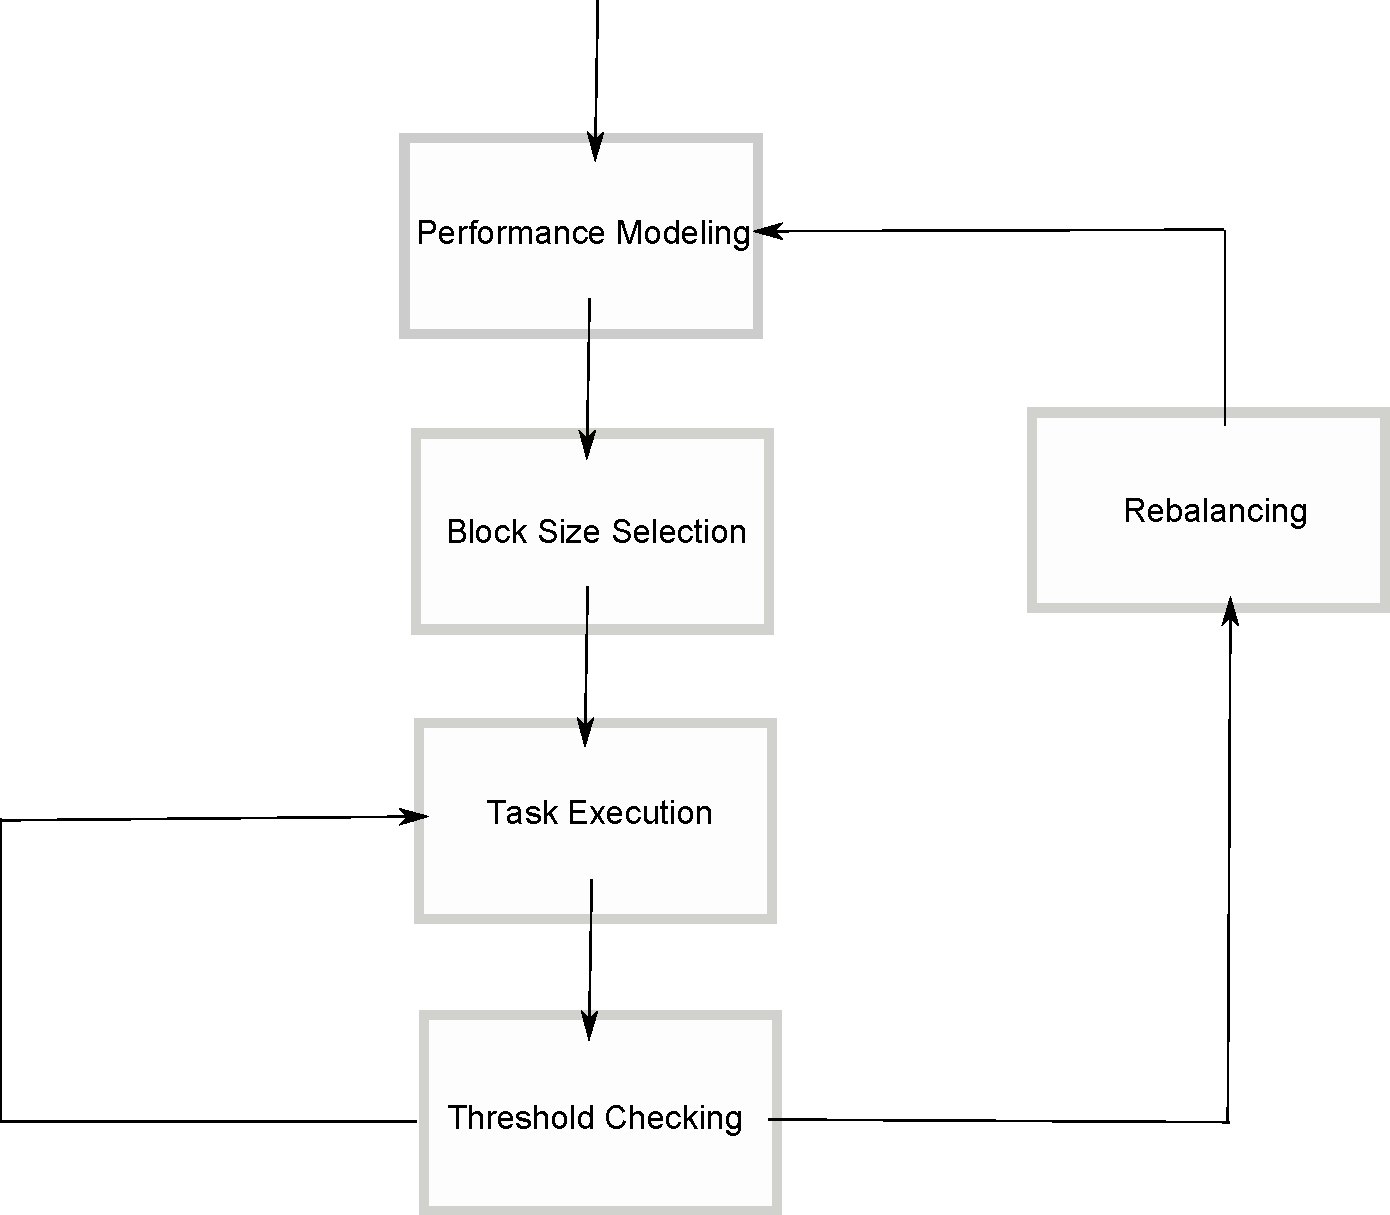
\includegraphics[width=.8\linewidth]{Fluxo.pdf} 				
	\caption{Flowchart of the algorithm}
	\label{fig: fluxo1}
\end{figure}

\begin{figure}[!t]
	\centering
			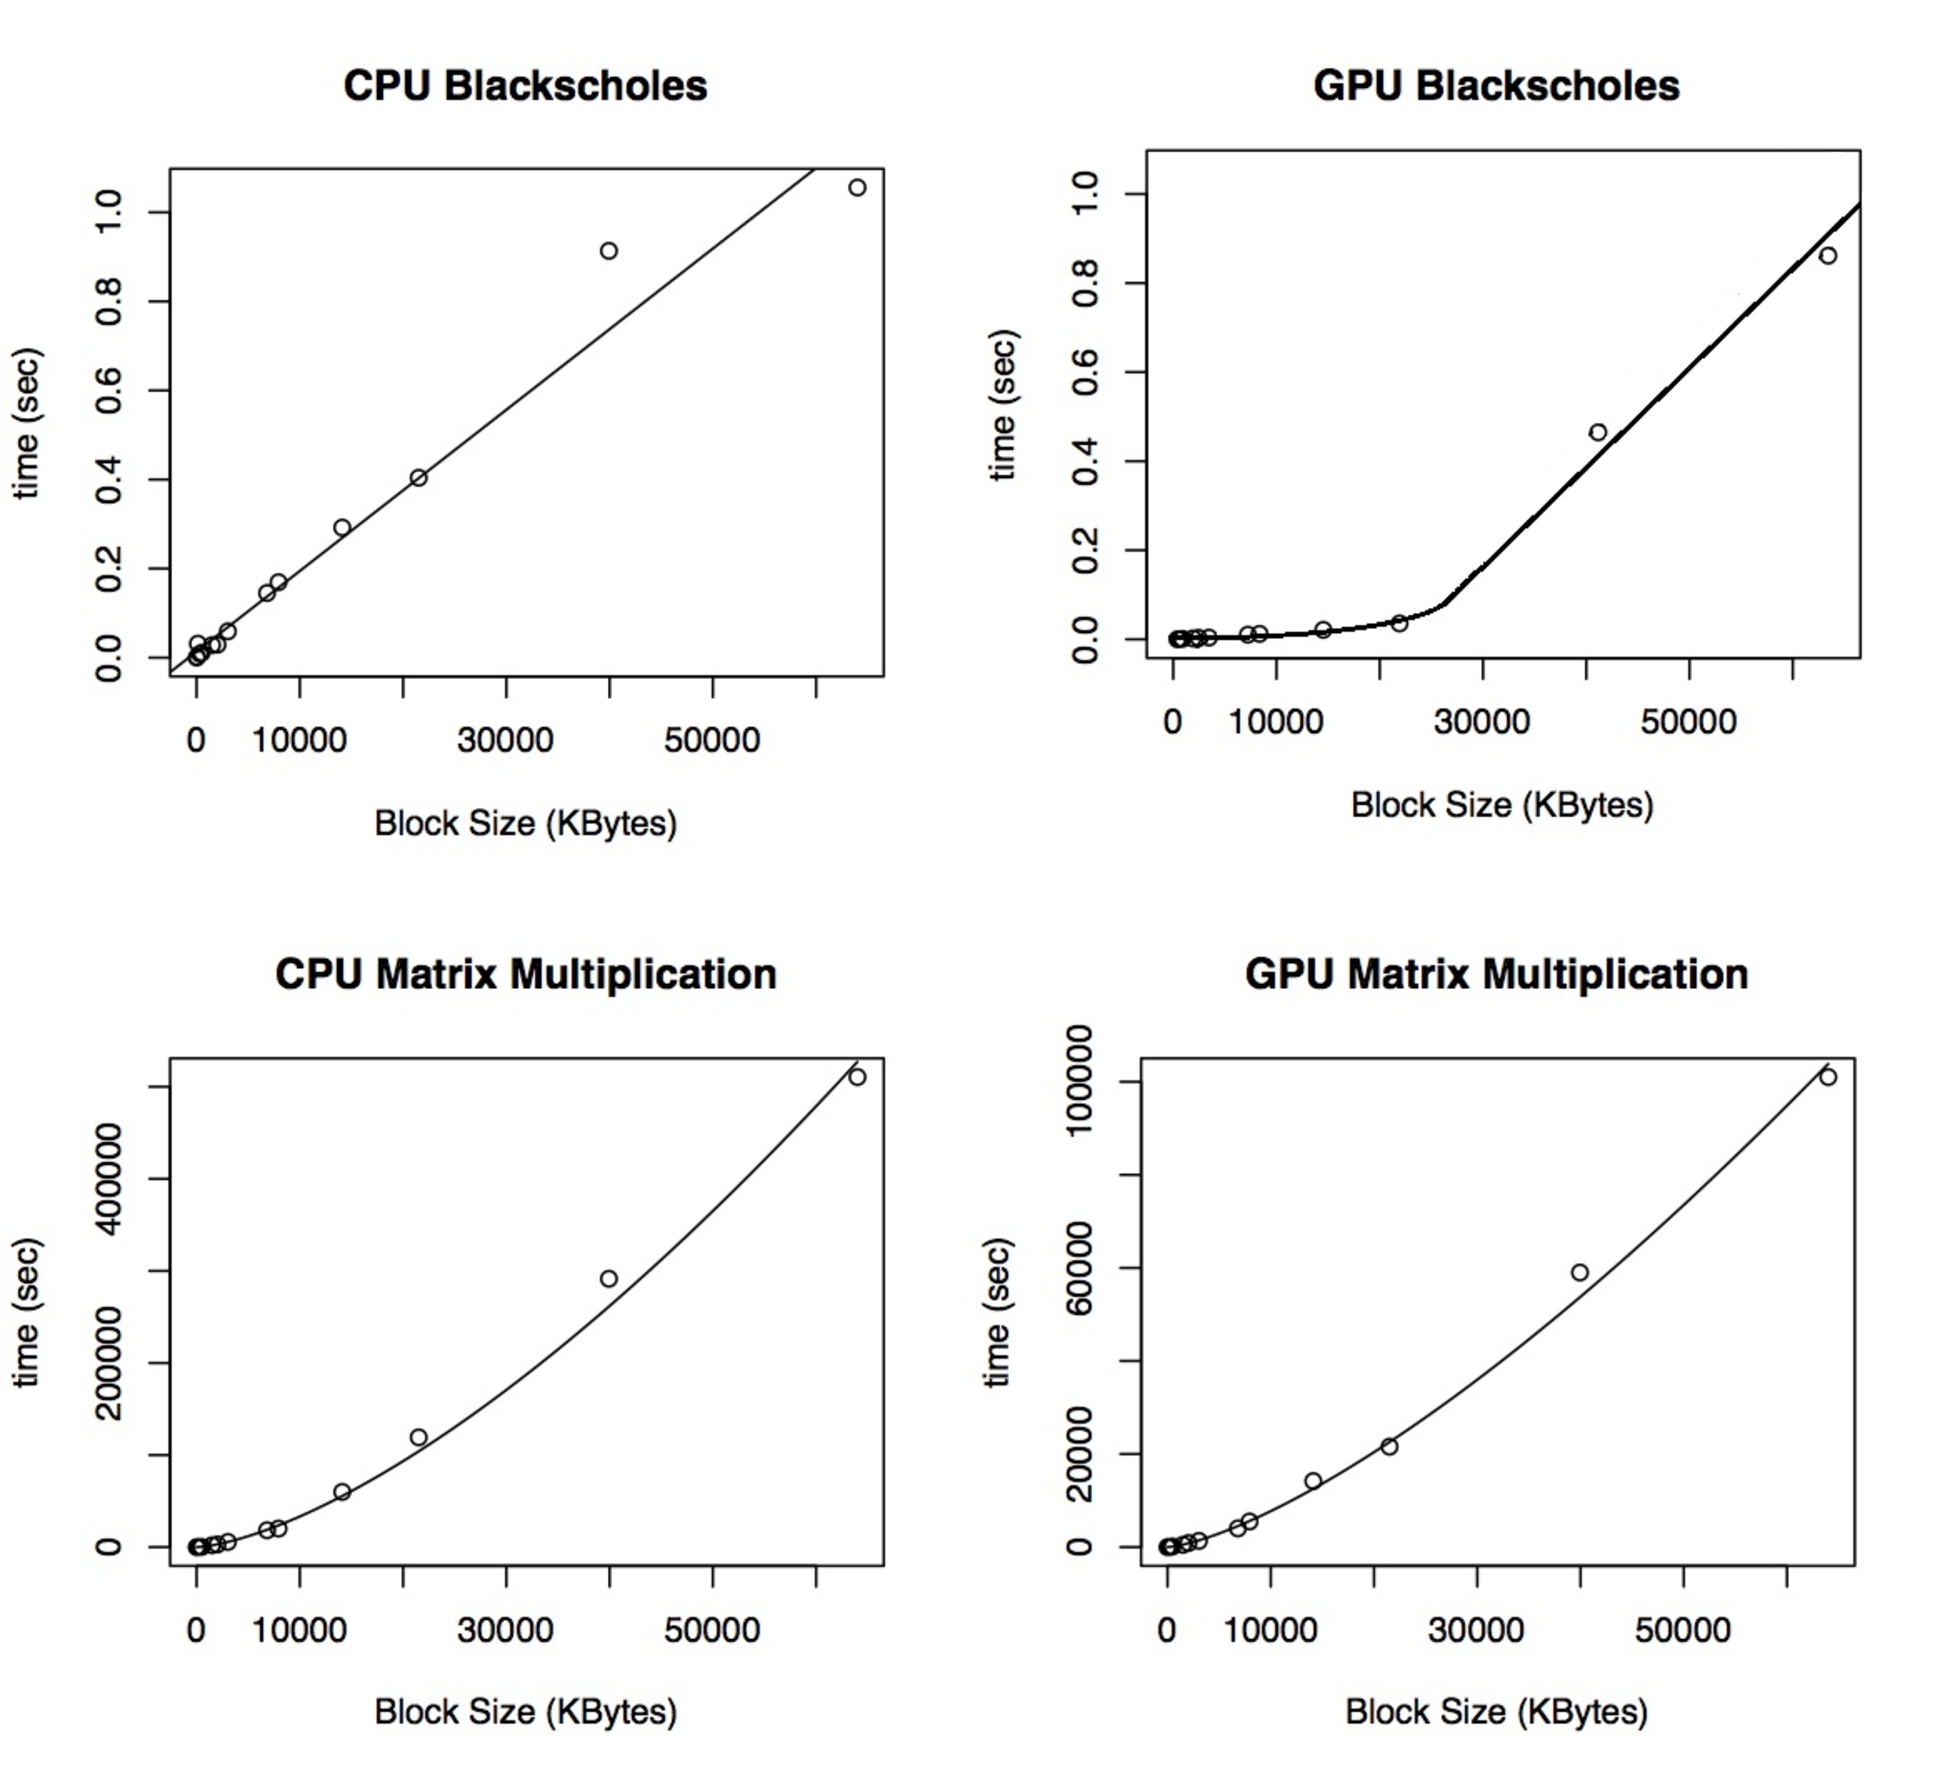
\includegraphics[scale=0.25]{CPUVersusGPULinear2_Ajustado.pdf} 				
	\caption{GPU and CPU processing times for different block sizes.}
	\label{fig: CPUVersusGPU1}
\end{figure}


%\vspace{0.2cm}
% RYC1029: Modifiquei toda a seção. Veja se o que escrevi está correto,
% especialmente a parte do coeficiente de correlação -> está correto :-)
%\paragraph*{Processor performance modeling.} 
\subsection{Processor performance modeling}

In this phase, the algorithm devise a performance model for each processor based on some initial benchmarks. The algorithm 
constructs a function $P_p[x]$, which represents the execution time of a block
of data of size $x$ on processor $p$. For this, it executes blocks of different
sizes on each processor and interpolate the curve that better fits these points.

A block of size $initialBlockSize$, an initial guess defined by the user, is initially allocated
and executed on each processor. After executing the first block, the algorithm
selects the processor with the earliest finish time $t_f$ and double the block
size for this processor. On the other processors, with finish times $t_k$, we
select blocks of size $initialBlockSize * t_k / t_f$. This procedure is repeated
until generating four points per curve. This process corresponds to (1) in
Figure~\ref{fig: algoritmo}, which shows a schematic view of processor
performance modeling part.

The algorithm then follows the step (2) of Figure~\ref{fig: algoritmo}, where it
tries to fit a curve in the existing points using the least squares fitting
method. If the coefficient of determination is greater than 0.7 for all
processors, the algorithm considers the fit as a ``good enough'' approximation and finishes this
phase. Otherwise, it generates more points in the curve following the previous
procedure.
 

% RYC1029: Cade o texto onde você explica os tipos de funções e combinações que
% usadas no fitting??? Não tínhamos discutido este ponto e você incluído na
% qualificação? -> adicionado
We devise the best fit curves using the well-known method of \textit{least
  squares}, using a function of the form:

\begin{equation}
 y(x) = a_{1} f_{1}(x) +  a_{2} f_{2}(x) + ... + a_{n} f_{n}(x) 
\label{eq: least}
\end{equation} 

where $ f_i (x) $ corresponds to the following set of functions $x$, $x^2$, $x^3$, $e^x$, $x$ and the combinations $x \cdot e^x$ and $x \cdot lnx$.
 % If the model does not fit into one of the functions described, the function that approximates the model is used.
 % The values ​​of $a_i$ are given by the least squares method itself, as set value. The method of least squares tests for each function and the one with the smallest error is selected.

Figure~\ref{fig: CPUVersusGPU1} shows sample processing time measurements for a
GPU and a CPU for different block sizes and two applications. We can see that
the curves can be approximated by different types of functions.
% RYC1029: Colocar as funções que aproximaram cada gráfico.

\begin{figure}[!t]
	\centering
	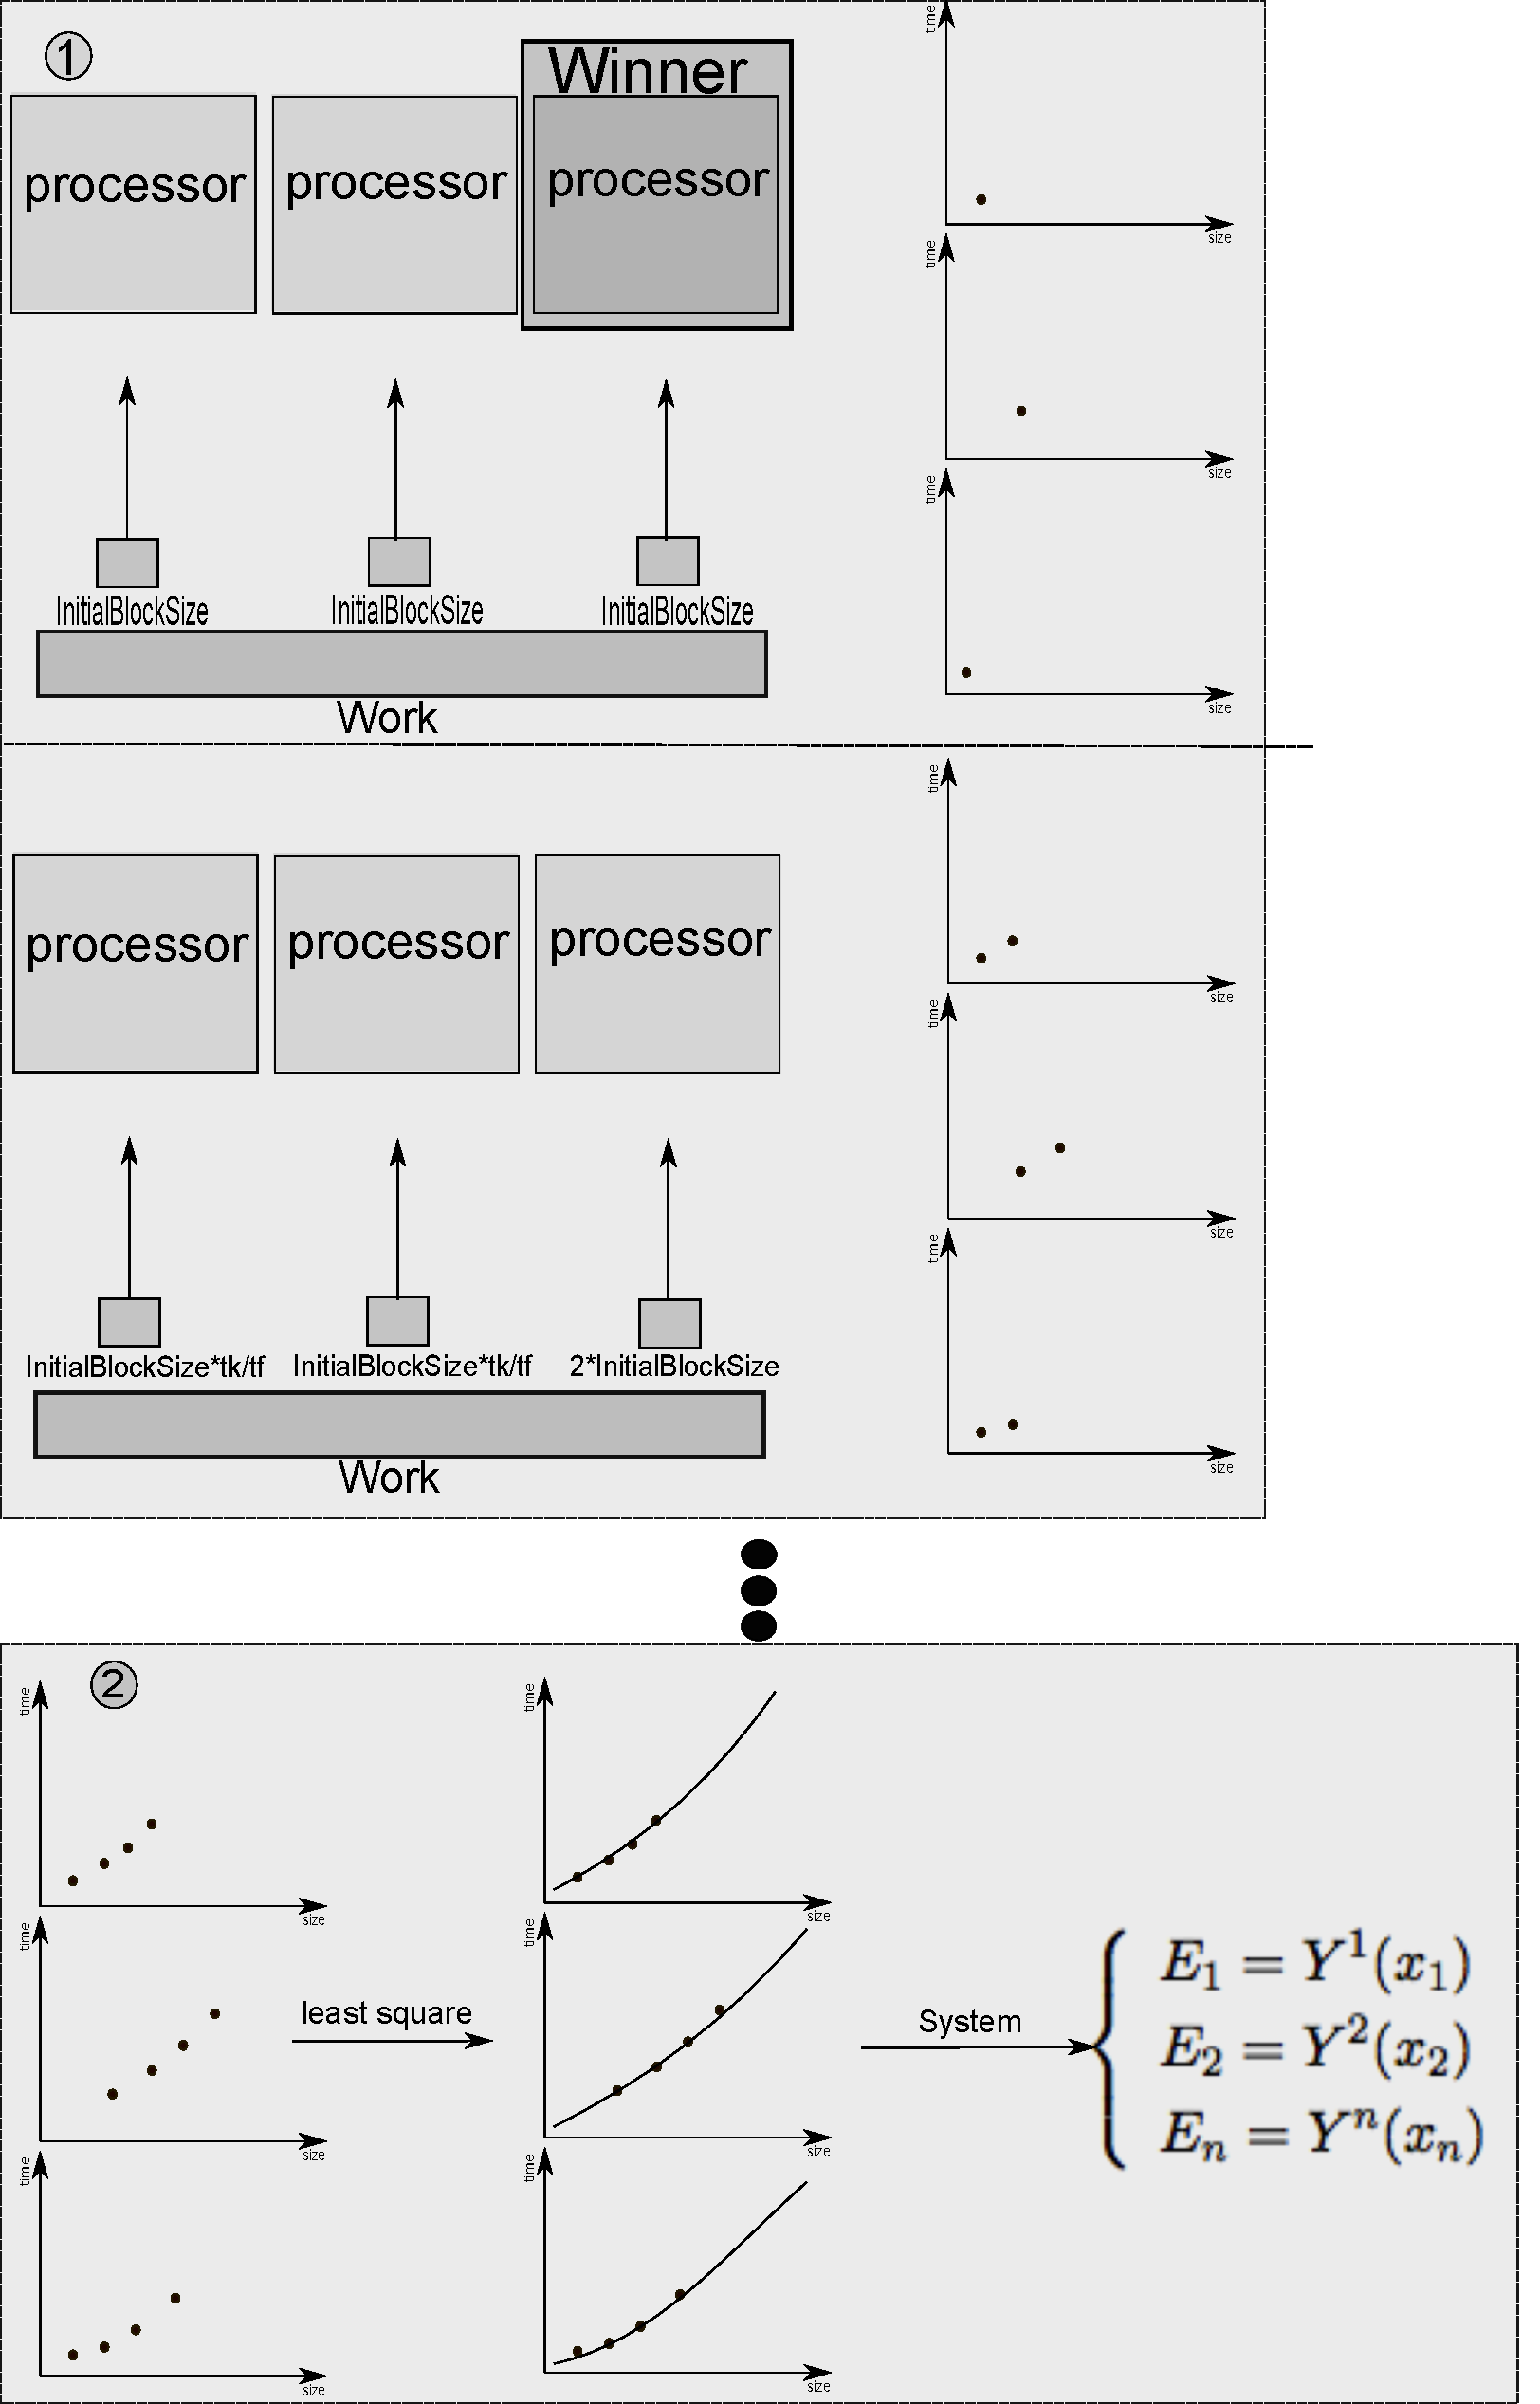
\includegraphics[scale=0.25]{NovaFigura_Algoritmo.pdf} 
	\caption{Performance modeling phase.}
	\label{fig: algoritmo}
\end{figure}

% RYC1029: A Figura 2 está com erros. Seria melhor ela representar apenas a
% parte da modelagem de desempenho, dado que ela está nesta seção. Eu juntaria a
% parte (1) com a (2), que é repetida por 4 vezes e só então que prossegue para
% a (3) e (4), que eu juntaria em um item só (3) + (4). Se na (4) o erro das
% funções for menor que um limiar, esta parte termina. Se não for, volta para o
% passo (2). Além disso, essa figura da parte (1) + (2) não ajuda em muita
% coisa. Precisaria repensar como deixá-la melhor e de um jeito que ajude o
% leitor. Passei a descrição da figura para junto do texto explicando o
% algoritmo. -> Mexi na figura, melhorou?



%Using a search method, a solution is found, with the restriction time. The time
%requires to be the same for all processors. The result is block of optimum
%size. If the cluster undergoes a change in behavior, and the time difference
%among the processors exceeds a threshold, the process and the calculation is
%redone.


\begin{algorithm}

\caption{Processor performance model}
\label{algModel}

\begin{algorithmic}		

\STATE \textbf{function}~determineModel()

\STATE $blockSizeList \leftarrow initialBlockSize;$
\WHILE{$fitValues.error \geq 0.7$}
		\STATE $finishTimes$ = executeTasks($blockSizeList$);
	        \STATE $blockSizeList$ = evaluateNextBlockSizes($finishTimes$);
		\STATE $fitValues$ = determineCurveProcessor();
\ENDWHILE

return $fitValues$;

\end{algorithmic}
\end{algorithm}

% RYC1029: O erro é 0.5 ou 0.7? No texto anterior estava 0.7 e no algoritmo está
% 0.5 -> 0.7, acertei o valor

The pseudo-code for this phase is shown in Algorithm~\ref{algModel}. This code
is executed in a single node, called \emph{master node}. Variable
$blockListSize$ contains the size of the blocks assigned to each processor and
is initialized with an estimation ($initialBlockSize$) given by the
user. Variable $fitValues$ contains results from the last least square fitting,
including the $error$ in the fitting, which is initialized as
$+\infty$. Iteratively, the algorithm sends chunks of data to each processor and
measures the time that each one spent to process them.  These results are used
to determine the block size for each processor in the next iteration and to
calibrate the model. The loop stops when the computed model have a bounded
(``good enough'') error or when the submitted block sizes reaches 20\% of the
total application data.

%\vspace{0.2cm}
%\paragraph*{Optimal block size selection} 
\subsection{Optimal block size selection}
In this phase our algorithm determines 
the optimal block size for each processor with the objective of providing blocks
with the same execution time on each processor.

Consider that we have $n$ processors and a input data of size $Z$. The algorithm assigns
a data chunk of size $x^g$ for each processor $g=1,...,n$, corresponding to a
fraction of the input data, such that $\sum_{g=1}^n x^g = Z$. We denote as
$E^g(x^g)$ the execution time of task $E$ in the processor $g$, for input of
size $x^g$. To distribute the work among the processors, we find a set of values
	
\begin{equation}
	X = \{ x^g \in \mathbb{R}:[0,1] \mid \sum_{g=1}^n x^g = Z \}
	\label{eq: totalResultado}
\end{equation}

that minimizes $E_1(x_1)$ while satisfying the constraint

\begin{equation}
	E_{1} = E_{2} = ...= E_{n}
	\label{eq: Restricao}
\end{equation}

which indicates that all processors should spend the same amount of time
performing the processing. To determine the set of values $x$, we solve the
system of fitted curves for all processors, determined in the performance
modeling part, and given by:

\begin{equation}
	\left\lbrace
	\begin{array}{ll}
		\displaystyle E_{1} = f(x_{1})  \\
		\displaystyle E_{2} = f(x_{2})   \\
		\displaystyle E_{n} = f(x_{n}) 
		\label{eq: system}
	\end{array}
	\right.
\end{equation}

The equations system is solved applying an interior point line search filter
method~\cite{point}, which finds the minimum solution of a convex equation set,
subject to a set of constraints, by traversing the interior of its
feasible region.

% RYC1029: Temos no começo uma grande quantidade de dados, pegamos uma parte
% destes dados Z e distribuimos entre os processadores. Como este Z é
% determinado? Pegamos uma porcentagem do total de dados? Usa-se valores que
% estão dentro dos valores medidos na parte de performance modelling?

%Isso eu tive que definir, baseei-me no algoritmo HDSS. O Z não pode exceder 20\% do tamanho total do problema. 

%\vspace{0.2cm}
%\paragraph*{Execution and Rebalancing}  
\subsection{Execution and Rebalancing}
After determining the task sizes, the scheduler sends a block of the selected
size $x_i$ for each processor $i$. When a processor finishes executing a task,
it requests another task of the same size. The processors then continue the
execution asynchronously, until completing all the tasks.

% RYC1029: Luis -> completar o XXX abaixo.
The scheduler also monitors the finish time of each task. If the difference in
finishing times $t_i$ and $t_j$ between any two tasks of processors $i$ and $j$
goes above a threshold, the rebalancing process is executed. Small thresholds
may cause excessive rebalancing while large thresholds may tolerate larger
imbalances that will cause processor idleness. The threshold must be
determined empirically; values of about 10\% of the execution time of a single
block resulted in a good trade-off in practice.


During the rebalancing, the scheduler synchronizes the processors and apply the
processor performance modeling algorithm to fit the best curves for the
functions $P_p[x]$ updated with the execution times. The optimal block size
selection routine is then applied to determine new block sizes $x_i$ for each
processor $i$.

\begin{figure}[!t]
	\centering
			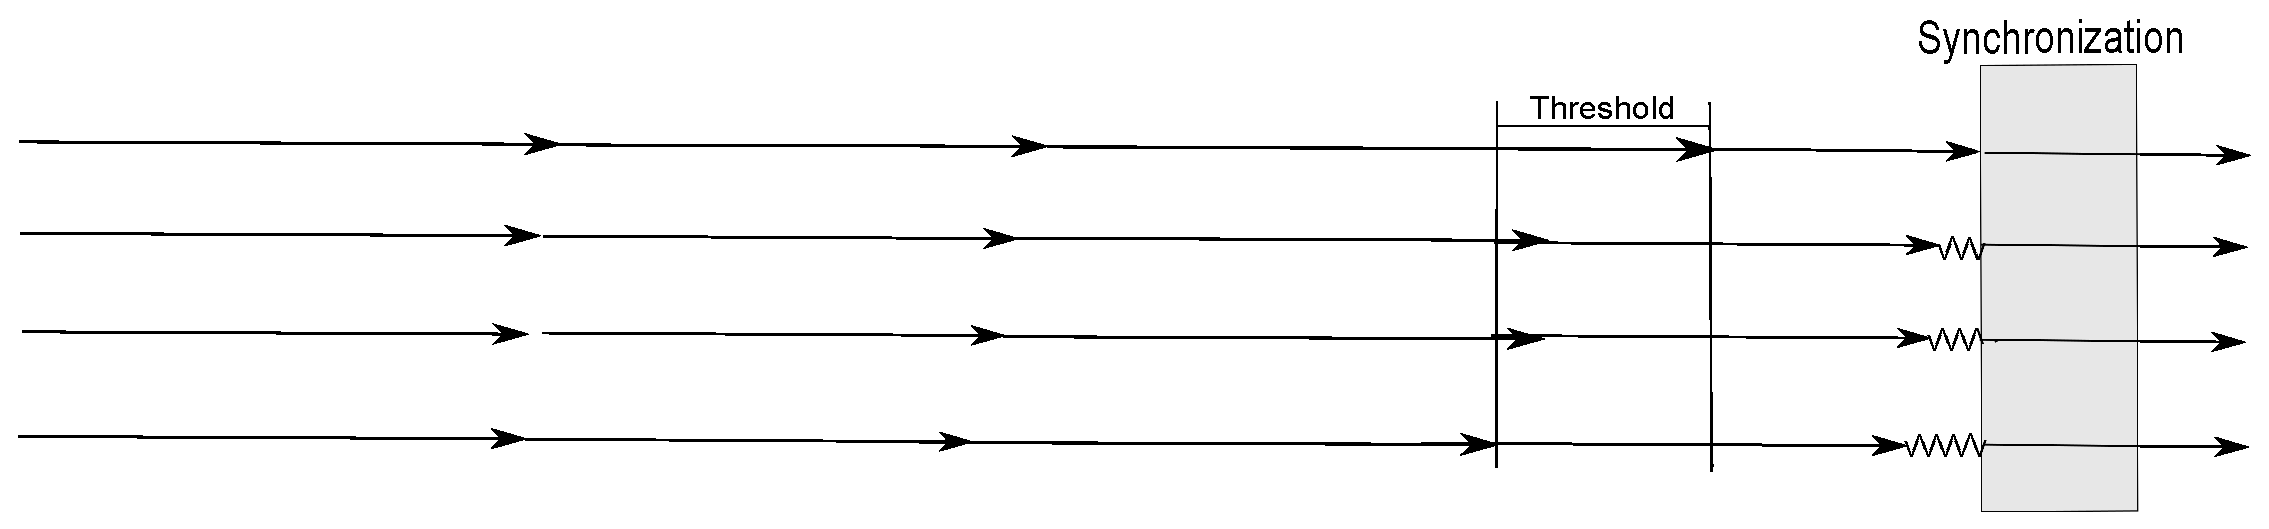
\includegraphics[scale=0.22]{DiagramaArtigo.eps}
	\caption{Execution of tasks by four processors. The finish time
         difference of two tasks was above a threshold, which caused a
          rebalancing of the task sizes.}
	\label{fig:Diagrama}
\end{figure}

% RYC1029: A figura ainda está toda torta, com as tarefas demorando tempos
% aleatórios para executar. Capriche mais na figura, fazendo os tempos de
% execução de cada tarefa proporcional, assim como o aumento do erro. Também
% precisa colocar uma seta no início de cada linha e uma logo depois da
% sincronização. Também precisa incluir onde o algoritmo de rebalancemanto é
% executado. -> Arrumei a figura, tem mais algum problema?

Figure~\ref{fig:Diagrama} depicts the execution of four processors, where
each arrow indicates the start of a task execution. The tasks start
synchronized, but their finish times start to diverge until the differences
reaches a threshold. In this case, all threads are synchronized, and the new
task sizes are recalculated for each processors. The task executions then
restart.

%\vspace{0.2cm}
%\paragraph*{Complete algorithm} 
\subsection{Complete algorithm}
Algorithm~\ref{alg1} shows the pseudo-code of the scheduling algorithm. The
$determineModel$ function, shown in Algorithm~\ref{algModel} returns the
performance model for each processor into variable $fitValues$. The algorithm
then solves the system of equations contained in $fitValues$ to determine the
best distribution $X$ of task sizes for each processor. It then distributes
tasks of different sizes for each processor in the system.

\begin{algorithm}

\caption{Complete algorithm}
\label{alg1}

\begin{algorithmic}		

\STATE \textbf{function} LoadBalancingAlgorithm()

\STATE $fitValues$ = determineModel()
\STATE $X$ = solveEquationSystem($fitValues$);
\FOR {each $proc$ from processorList}
  \STATE distributeTasks($X$, $proc$);
\ENDFOR
\end{algorithmic}

\vspace{0.2cm}

\begin{algorithmic}		
\STATE \textbf{function} FinishedTaskExecution($proc$, $finishTime$)

\IF{there is data}

	\IF {$ $maxDifference($finishTime$)$ \geq threshold$}
		\STATE synchronize();
		\STATE $fitValues$ = determineCurveProcessor();
        \STATE $X$ = solveEquationSystem($fitValues$);
    \ENDIF
        
	\STATE distributeTask($X$, $proc$);
    
\ENDIF


\end{algorithmic}
\end{algorithm}

% RYC1029: Este algoritmo está errado, pois ele considera que a execução das
% tarefas é síncrona. O algoritmo que você implementou provavelmente é baseado
% em eventos (término de tarefas). Você precisa fazer o mesmo aqui. Em seguida,
% é preciso alterar o texto para refletir estas mudanças.

%Não sei como podemos alterar para eventos, o algoritmo dá a entender que é
% baseado a eventos, assim que a tarefa termina, é registrado o tempo no 
%vetor finishTime, e com base neste vetor é decidido se precisamos rebalancear.

When a processor finishes its task, it calls the function \texttt{FinishedExecution}, passing as parameters its finish time $finishTime$ and its identifier $proc$. If there is more data to process, the function checks the difference between the finish time of this processor with the previous ones. If this difference exceeds a defined threshold, the algorithm devises new curves for each processor performance model and solve the system of equations to determine a new distribution of tasks sizes for each processor. It then distributes the new task for the finished processor.

%%%%%%%%%%%%%%%%%%%%%%%%%%%%%%%%%%%%%%%%%%%%%%%%%%%%%%%%%%%%%%%%%%%%%%%%%%%

\section{Implementation}

The algorithms were implemented in the C language, using the StarPU framework.
StarPU~\cite{starpu} is a tool for parallel programming that supports hybrid
architectures like multicore CPUs and accelerators. The StarPU proposes an
approach of independent tasks based architecture. Codelets are defined as an
abstraction of a task that can be performed on one core of a multicore CPU or
subjected to an accelerator. Each codelet may have multiple implementations, one
for each architecture in which codelet can be performed using specific languages
and libraries for the target architecture. A StarPU application is described as
a set of codelets with data dependencies.

%The tool offers a set of scheduling policies that the programmer can choose
%according to the characteristics of the application. The most used is the static
%scheduling algorithm HEFT (Heterogeneous Earliest Finish Time), that schedule
%the tasks based on cost models of task execution.

% DC: o que eh um kernel? O conceito nao foi definido antes.
% For each device one codelet has been programmed with the characteristics of the
% devices. A codelet is a structure that represents a computational function. Such a
% codelet may contain an implementation of the same function on different
% architectures (e.g. CUDA and x86).  The applications were implemented by
% dividing the data set into tasks, implemented as codelets. The tasks are
% independent, with each task receiving a part of the input set proportional to
% the processor weight. Two codelets were implemented one for GPU/CUDA and one for
% CPU architecture.


%
% DC: acho que a descricao abaixo eh muito baixo nivel e nao auxilia na compreencao do algoritmo.
%
% There are data structures and functions that speed up the process of development. For example the function "double starpu\_timing\_now (void)"  return the current date in micro seconds, which makes it easier for the determination of measures runtime. In StarPU there is a data structure called "starpu\_sched\_policy" This structure contains all the methods que Implement a scheduling policy. 

We implemented our load-balancing algorithm in the StarPU framework. The StarPU
framework offers a rich API that allows one to modify and develop new scheduling
policies. For comparisons sake, we also implemented three other algorithms:
\emph{greedy}, \emph{Acosta} algorithm and \emph{HDSS}. The greedy consisted in
dividing the input set in pieces and assigning each piece of input to any idle
processor, without any priority assignment. Acosta algorithm~\cite{acosta},
described in Section~\ref{sec:ralated}, interactively finds a good distribution
of work between CPUs and GPUs based on the execution of the previous task.
Finally, The HDSS~\cite{HDSS} was implemented using minimum square estimation to
estimate the weights and divided into two phases: adaptation phase and
completion phase.

We used the IPOPT~\cite{point} library to solve the equations systems produced
by Equation~\ref{eq: system}. IPOPT (Interior Point Optimize) is an open source
software package for large-scale nonlinear optimization. It can be used to solve
general nonlinear programming problems.

% DC: cuidado ao usar o termo blackscholes (aplicacao de exemplo) e Black-Scholes (o nome do algoritmo) 
%=========================================================
\subsection{Applications}

For evaluating our algorithm, we adapted two applications from the CUDA
SDK~\cite{cuda} to execute using the StarPU framework, the \emph{blackscholes}
and \emph{matrix multiplication} applications. We have also evaluated the
algorithms using a (more complex) gene regulatory networks (GRN)
inference~\cite{borelli2013gene} application. We implemented the applications
using two codelets for each, containing the GPU and CPU implementations.

For the matrix multiplication, we distribute a copy of the matrix A to all
processing units and matrix B is divided according to the load-balancing scheme.
We used an optimized version of the matrix multiplication, which uses the GPU
shared memory. Multiplication of two $n \times n$ matrices has complexity
$O(n^3)$.

Black-Scholes is a popular financial analysis algorithm for calculating prices
for European style options. The Black-Scholes equation is a stochastic
differential equation that describes how, under a certain set of assumptions,
the value of an option changes as the price of the underlying asset changes. It
includes a random walk term, which models the random fluctuation of the price of
the underlying asset over time. The input is a vector of data that the options
should be calculated by applying a differential equation. The division of the
task consists in giving a range of the input vector to each thread. The
complexity of the algorithm is $O(n)$, where $n$ is the number of options.

%The Black-Scholes equation implies that the value of a European call option.
%The cumulative normal distribution function gives us the probability that a
%normally distributed random variable will have a value less than $x$. There is no
%closed-form expression for this function, and as such it must be evaluated
%numerically. It is typically approximated using a polynomial function. The idea is to calculate the Black-Scholes the greatest amount of possible options. Thus, the input is a vector of data that the options should be calculated by applying a differential equation. The division of the task is given a position of providing input vector to each thread. The complexity of the algorithm is $O(n)$.


Gene regulatory networks (GRN) inference~\cite{borelli2013gene} is an important
bioinformatics problem in which the gene interactions need to be deduced from
gene expression data, such as $microarray$ data. Feature selection methods can
be applied to this problem and are composed by two parts: a search algorithm and
a criterion function. This application was developed as a parallel solution
based on GPU architectures for performing an exhaustive search of the gene
subset with a given cardinality that best predict a target gene. The division of
work consisted in distributing the gene sets that are evaluated by each
processor. The complexity of the algorithm is known to be $O(n^3)$, where $n$ is
the number of genes.


%%%%%%%%%%%%%%%%%%%%%%%%%%%%%%%%%%%%%%%%%%%%%%%%%%%%%%%%%%%%%%%%%%%%%%%%%%%

\section{Results}


\subsection{System Configuration}

% DC: corrigir as referências quebradas -> não achei
We used four machines with different configurations (shown in
Table~\ref{table:machines}), to evaluate our algorithm. We performed the
experiments using four scenarios: only one machine (A), two machines (A, B),
three machines (A, B, C) and four machines (A, B, C and D). Note that some
boards, such as GTX 295 and GTX 680 have two GPU processors on each.

To use the $k$ Stream Multiprocessors (SMs) from each GPU and the cores of the
each SM efficiently, we launched kernels with $k$ blocks and 1024 threads per
block. The number of available Stream Multiprocessors $k$ is \textbf{13, 14, 8,
  30} for Tesla K20c, GTX Titan, GTX 680 and GTX 295, respectively. We also used
all cores from the available CPUs, creating one thread per available core.

%Machine A has a CPU
%with 4 cores and two GPUs with 280 cores each. Machine B has 1 CPU with 6 cores
%and two GPUs with 1536 cores each. The machine C has 1 CPU with 6 cores and 1
%GPU with 2688 cores and finally the machine D has 1 CPU with 14 cores and 2 GPUs
%with X cores. 
 

%DC: corrigir última linha da tabela -> Foi corrigido
\begin{table*}[t]
\begin{scriptsize}
\caption{Machines configuration.\label{table:machines}}
\begin{center}

\begin{tabular}{|c|l|l|l|l|l|} \hline
\multicolumn{1}{|l|}{Machine} & \multicolumn{5}{|c|}{\textbf{Description}}                                                           \\ \hline
\multirow{2}{*}{A}          & \textbf{CPU Info} & Intel i7 a20   & 4 cores  @ 2.67 GHz  &   8 MB cache   & 8 GB RAM     \\ \cline{2-6}
                            & \textbf{GPU Info} & 2 x GTX 295 (2 GPUs)    & 2 x 240 cores / 30 SMs      & 223.8 GB/s  & 896 MB      \\ \hline
\multirow{2}{*}{B}          & \textbf{CPU Info} & Intel i7 4930K & 6 cores    @ 3.4 GHz & 12 MB cache       & 32 GB RAM   \\  \cline{2-6}
                            & \textbf{GPU Info} & GTX 680 (2 GPUs)        & 2 x 1536 cores / 8 SMs & 192.2 GB/s  & 2 GB      \\ \hline
\multirow{2}{*}{C}          & \textbf{CPU Info} & Intel i7 3939K & 6 cores    @ 3.2 GHz & 12 MB cache & 32 GB RAM      \\  \cline{2-6}
                            & \textbf{GPU Info} & GTX Titan      & 2688 cores / 14 SMs & 223.8 GB/s  & 6 GB        \\ \hline
\multirow{2}{*}{D}          & \textbf{CPU Info} & 2 x Intel Xeon E5-2690V2 & 10 cores   @ 3.0 GHz &            25 MB cache           & 256 GB RAM            \\  \cline{2-6}
                            & \textbf{GPU Info} & 4 x Tesla K20c & 2496 / 13 SMs       & 205 GB/s     & 6 GB                              \\ \hline 
\end{tabular}
\end{center}

\end{scriptsize}
\end{table*}

%---------------------------------------------------------------------------

\subsection{Matrix Multiplication}


We used the matrix multiplication application to evaluate the execution time
using different matrix sizes and number of machines of the following scheduling
algorithms: (1) our proposed algorithm, (2) Acosta algorithm, (3) HDSS, and (4)
Greedy. Our algorithm was configured with a threshold of 10\% of the execution
time and initial block size of 2048 elements. The initial block size of HDSS
algorithm was 1024 elements, a submatrix. The difference between the size of the initial block of the algorithms was obtained empirically, with tests, we was considered the best case.

\begin{figure*}[htb]
	\begin{center}
	\centering
		\subfigure[1 machine]{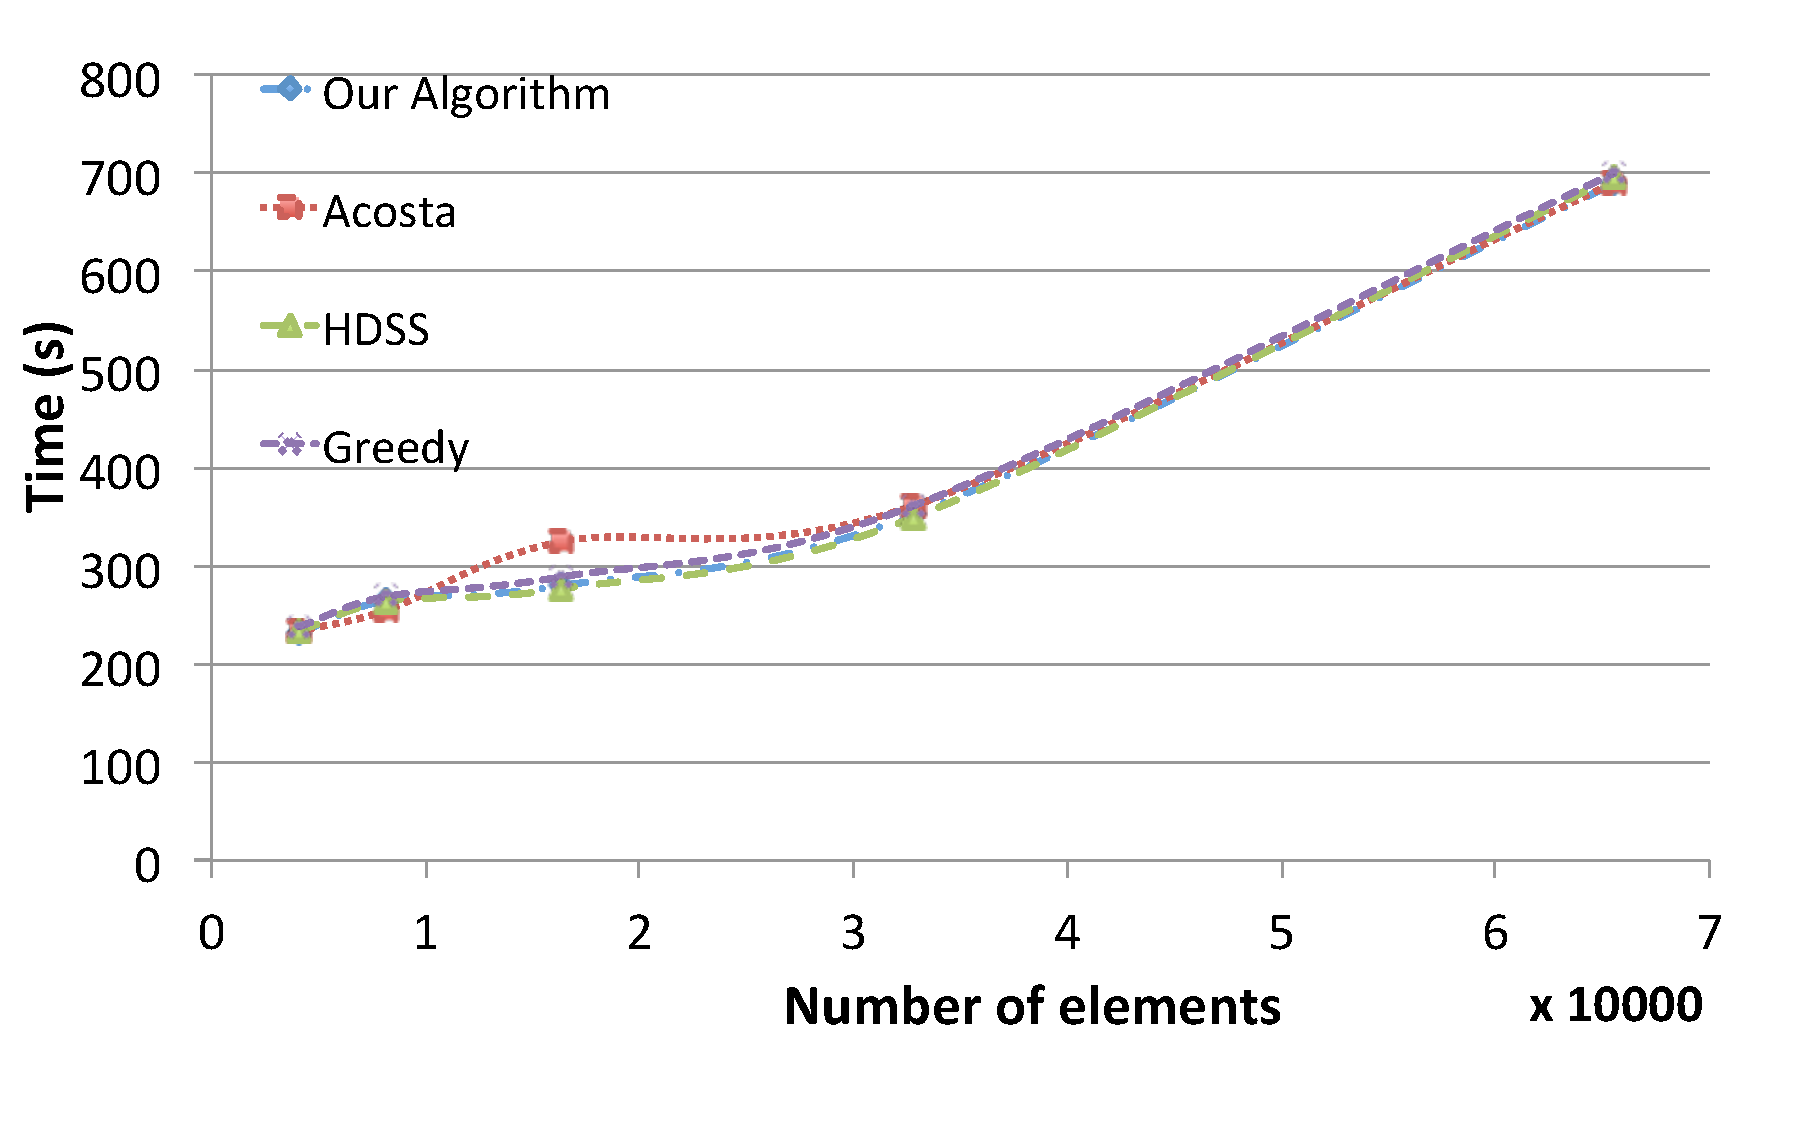
\includegraphics[height=3.3cm, width=4.52cm]{1machineN.pdf}}
	        \subfigure[2 machine]{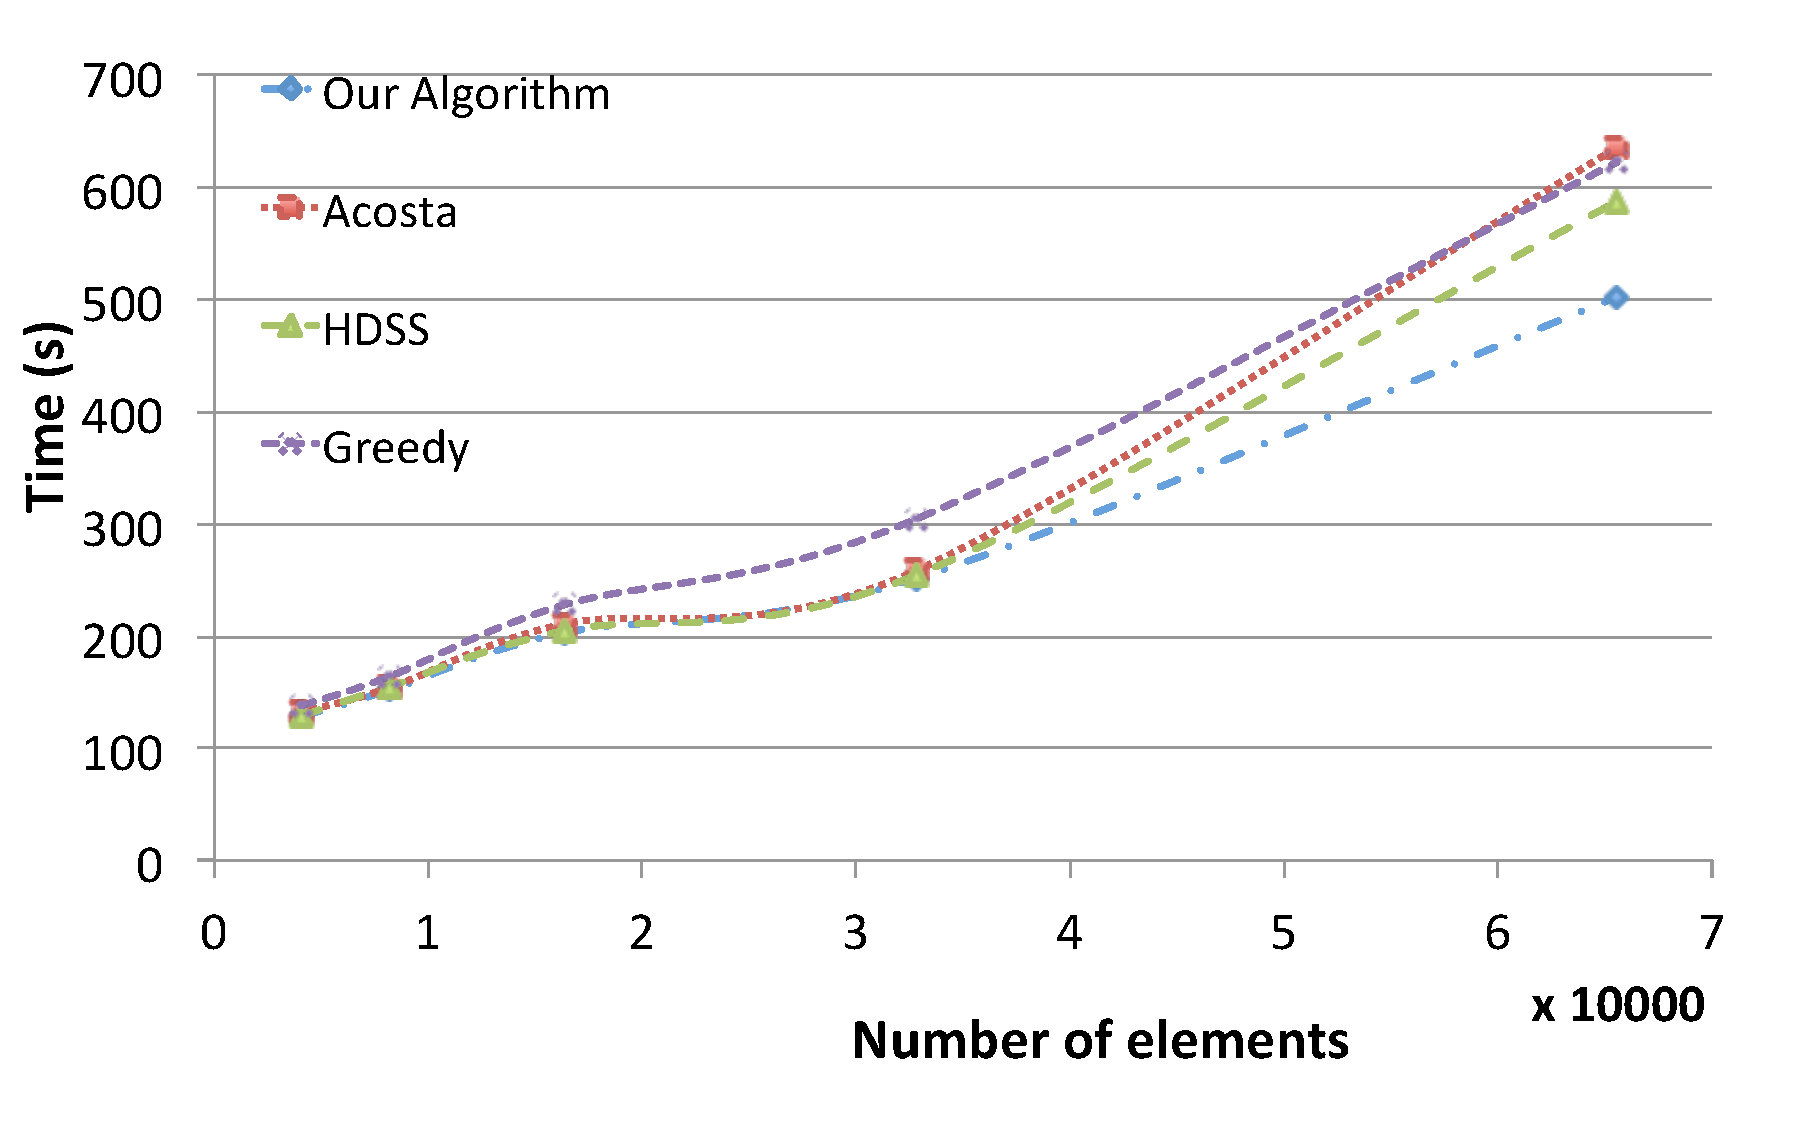
\includegraphics[height=3.3cm, width=4.52cm]{2machineN.pdf}}
		\subfigure[3 machine]{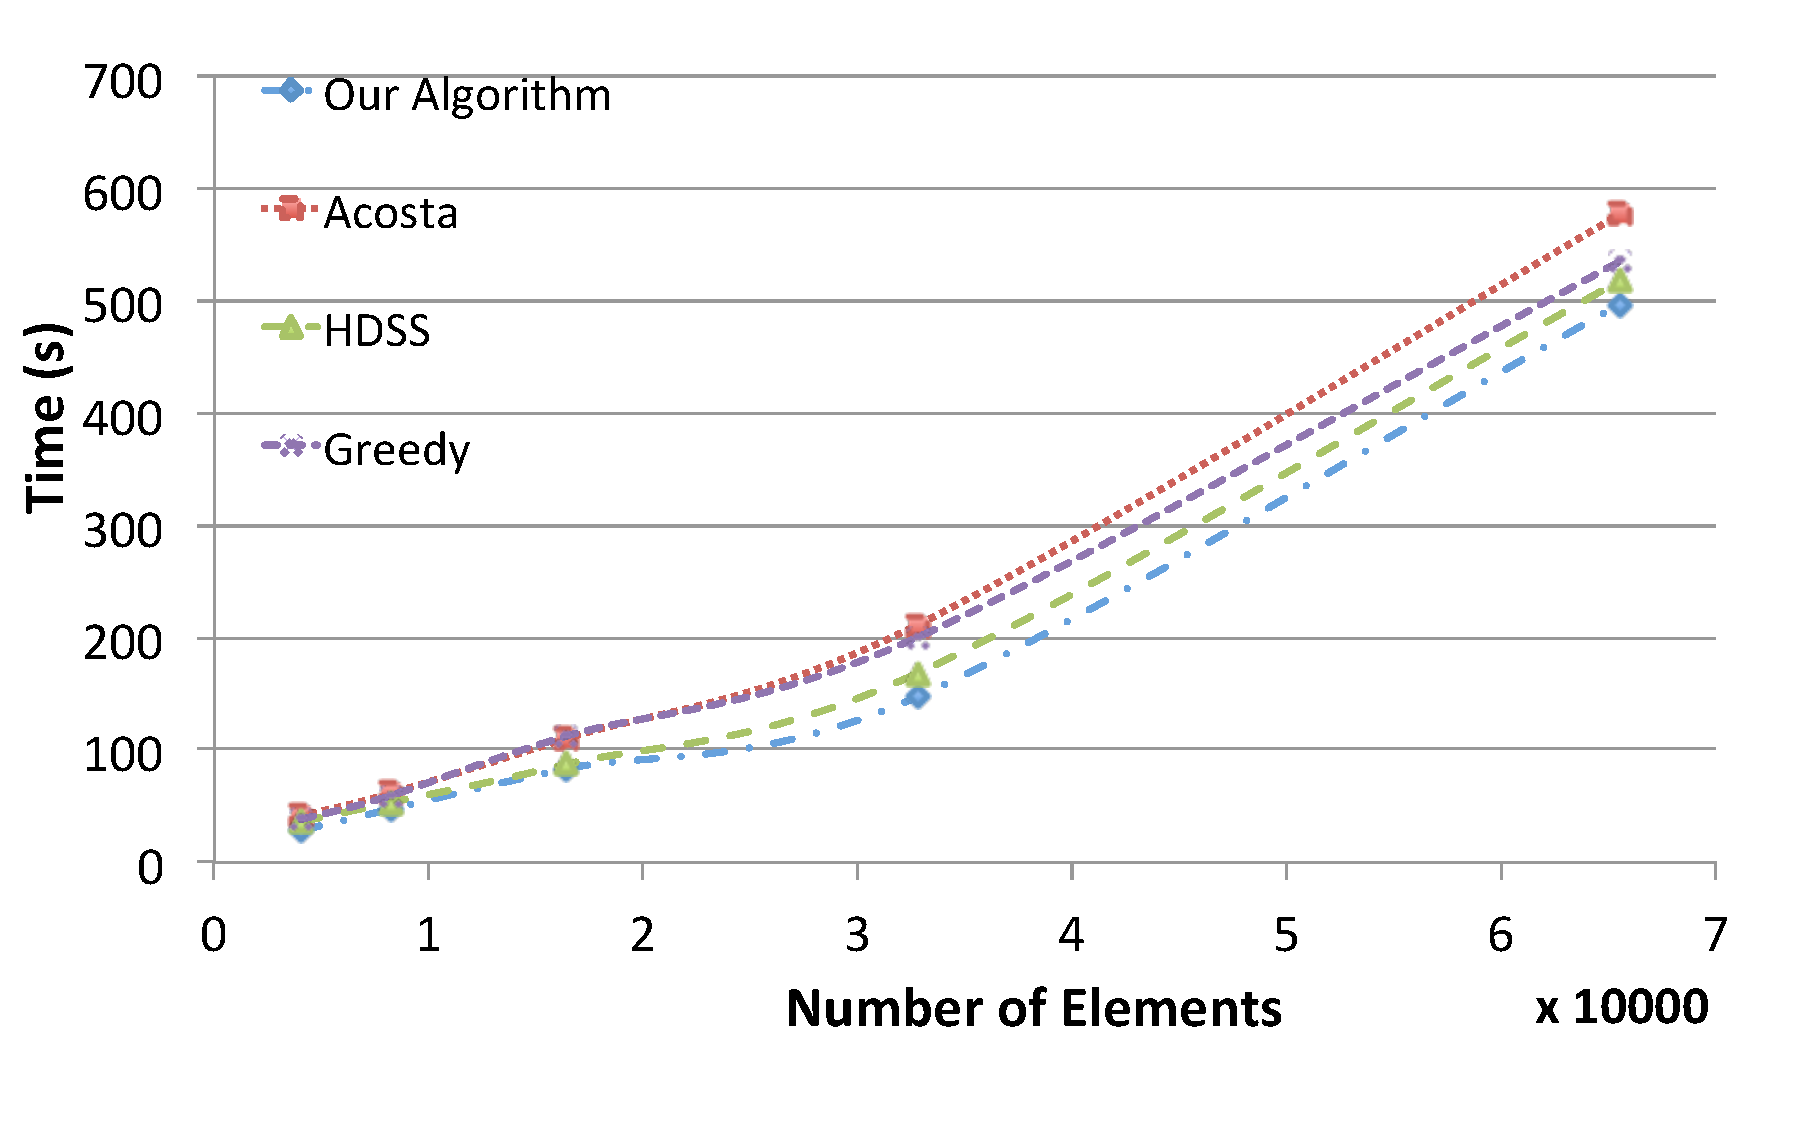
\includegraphics[height=3.3cm, width=4.52cm]{3machineN.pdf}}
		\subfigure[4 machine]{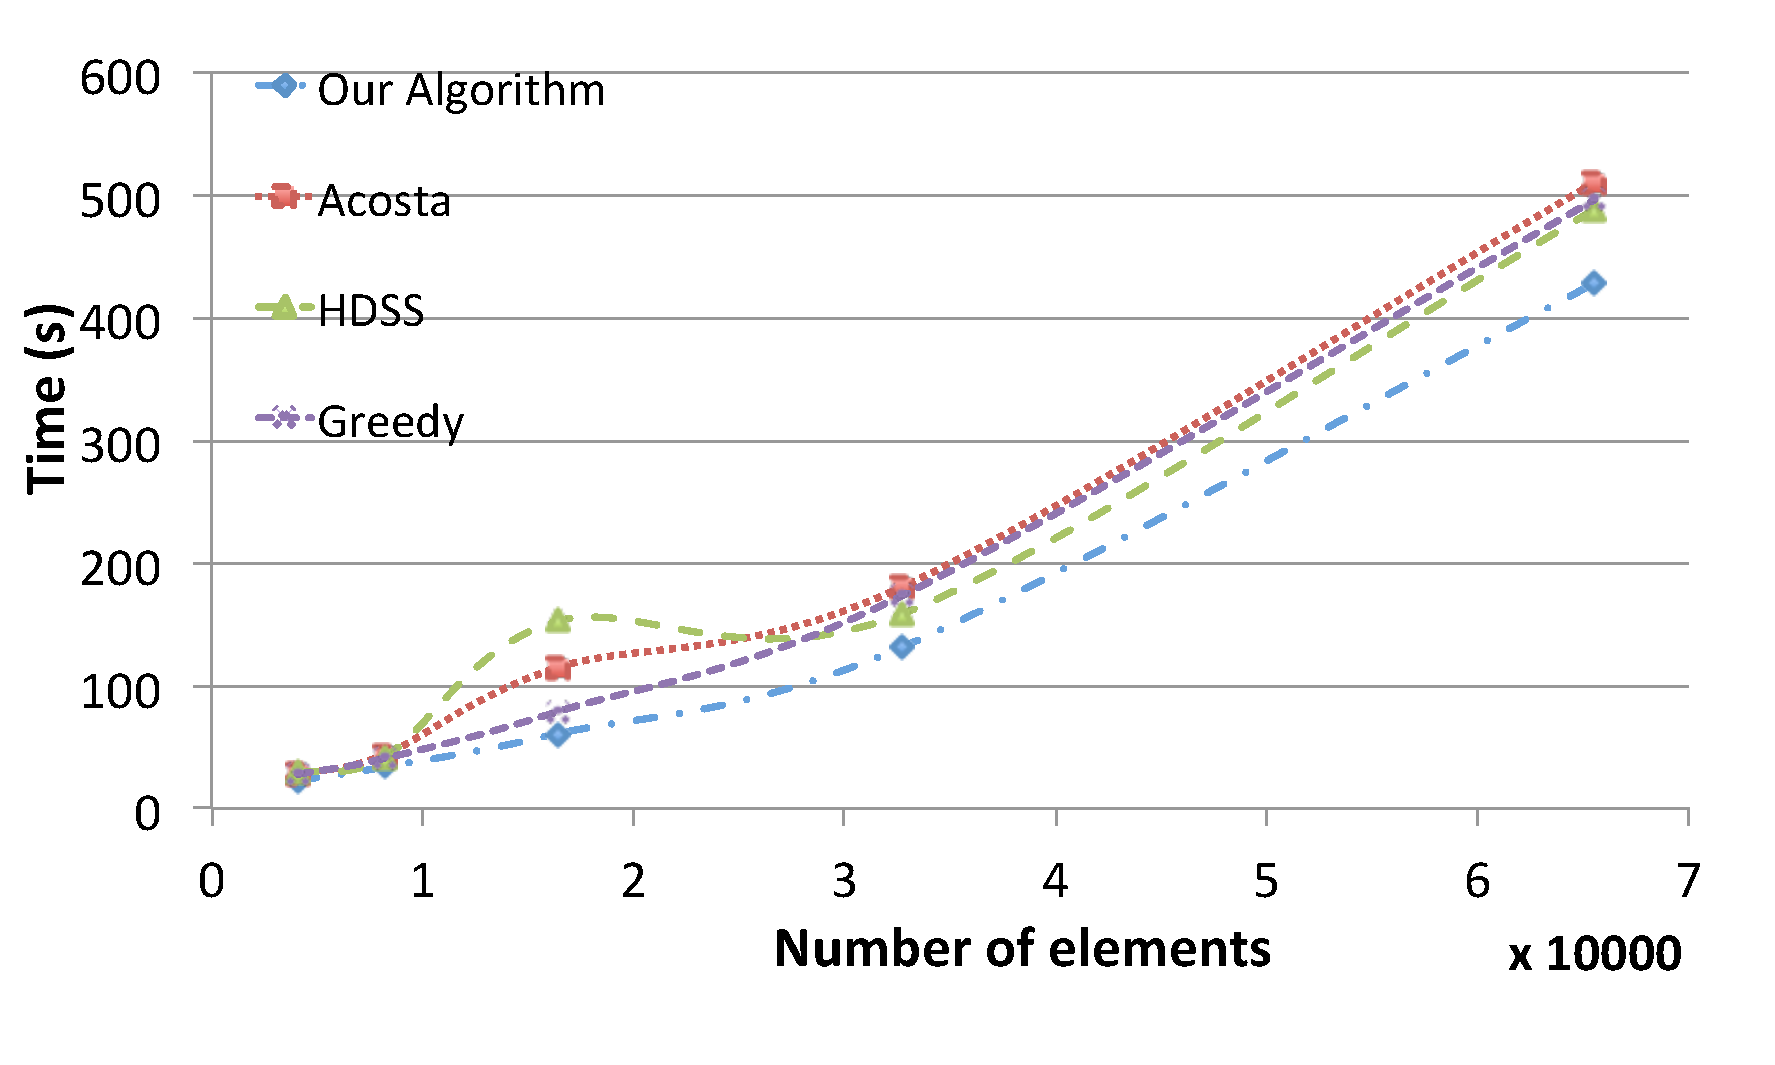
\includegraphics[height=3.3cm, width=4.52cm]{4machineN.pdf}}
			%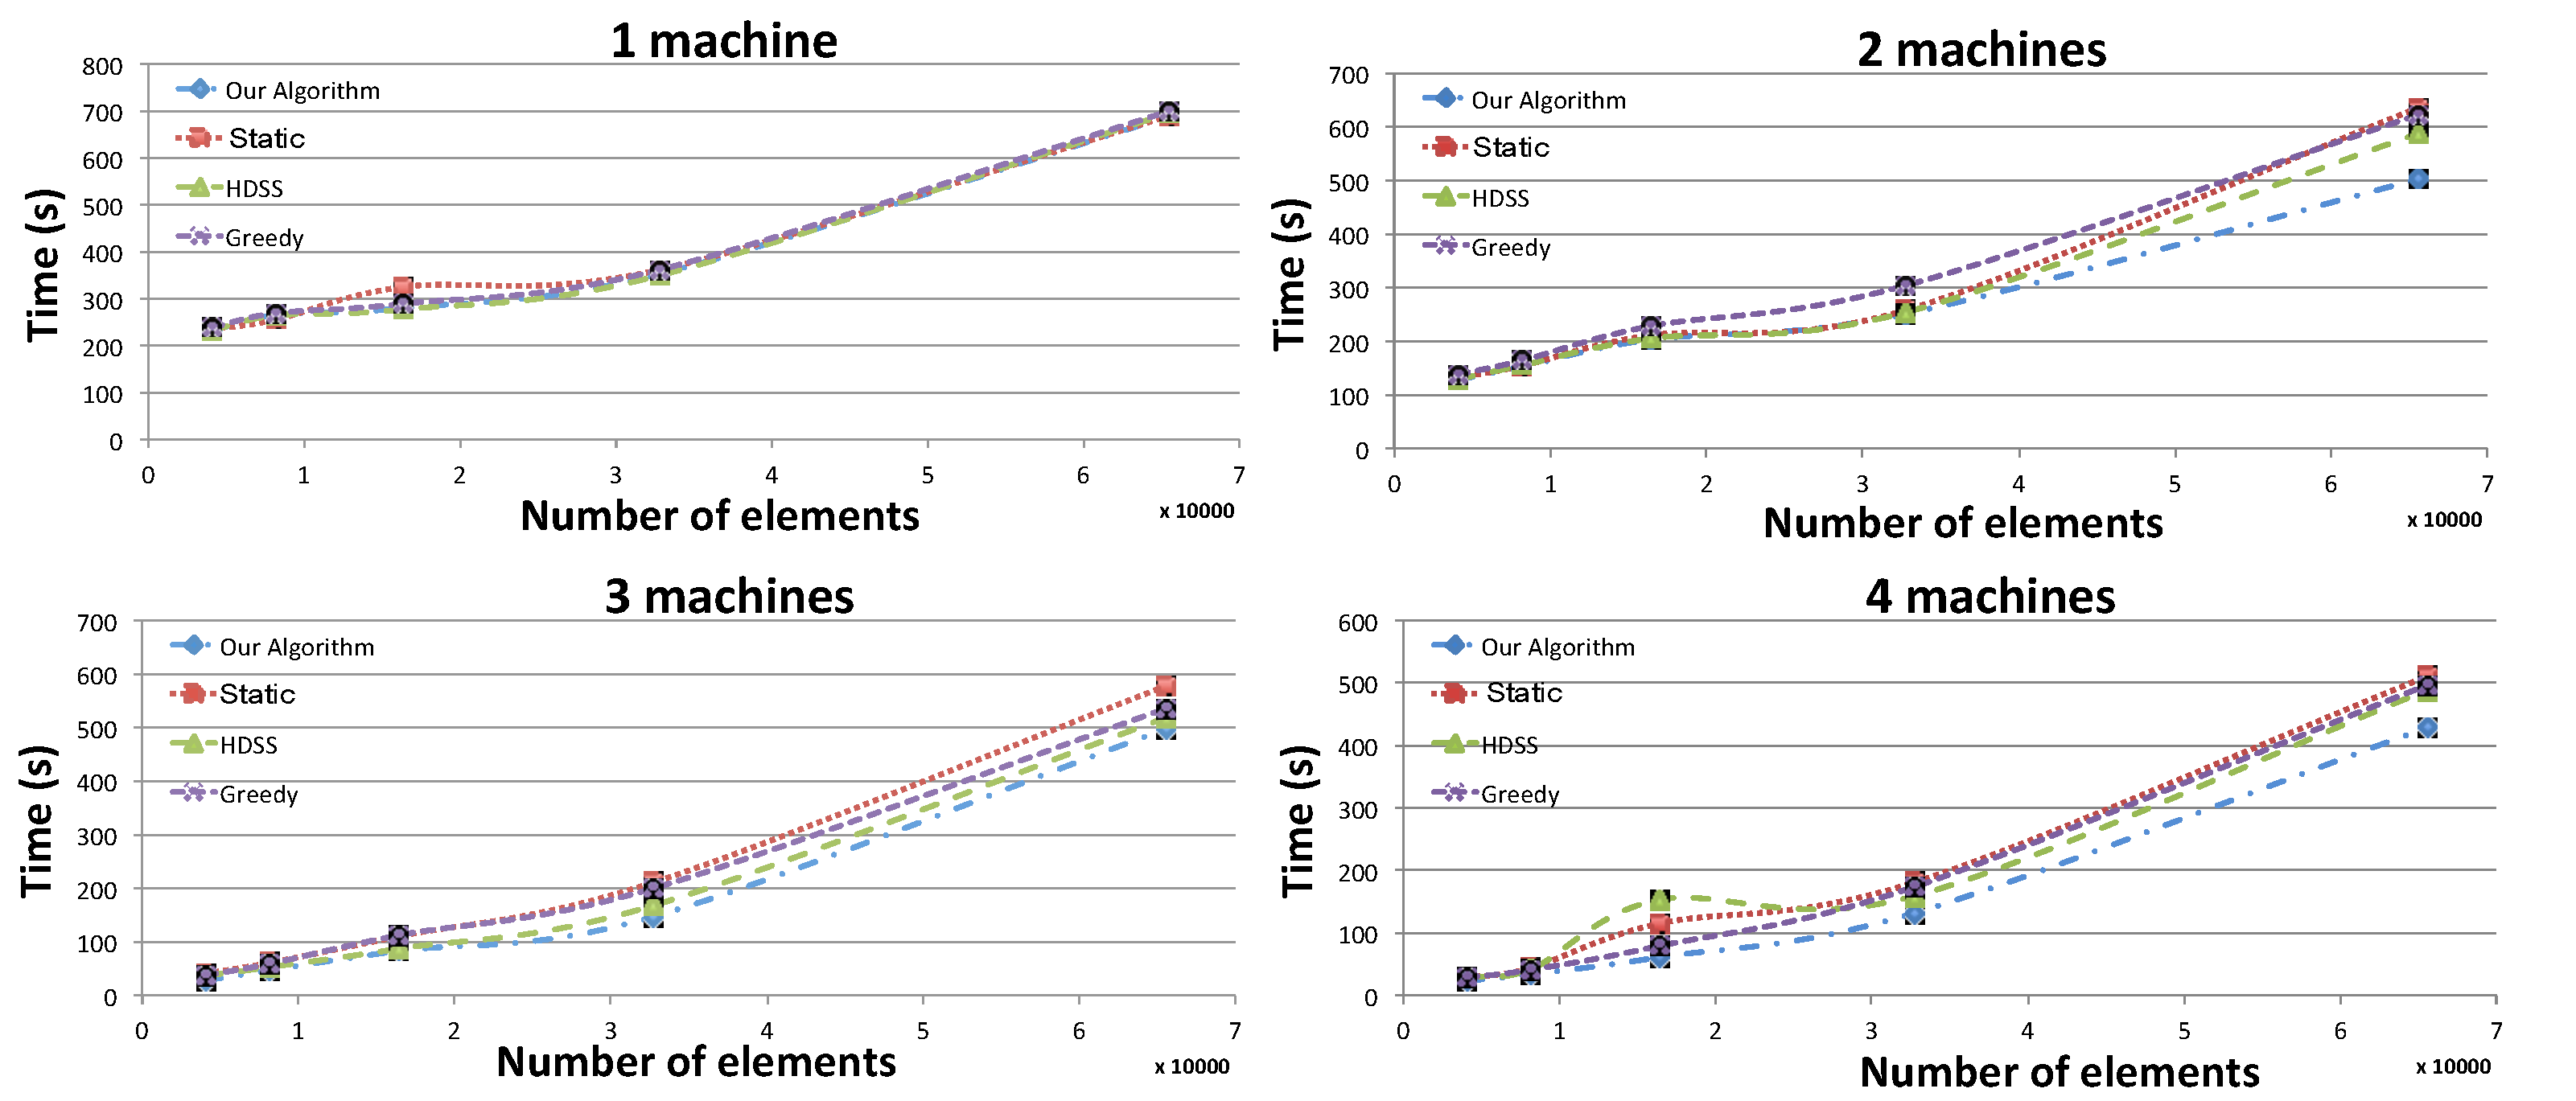
\includegraphics[scale=0.3]{SaidaMatriz.pdf} width=4.52cm
		%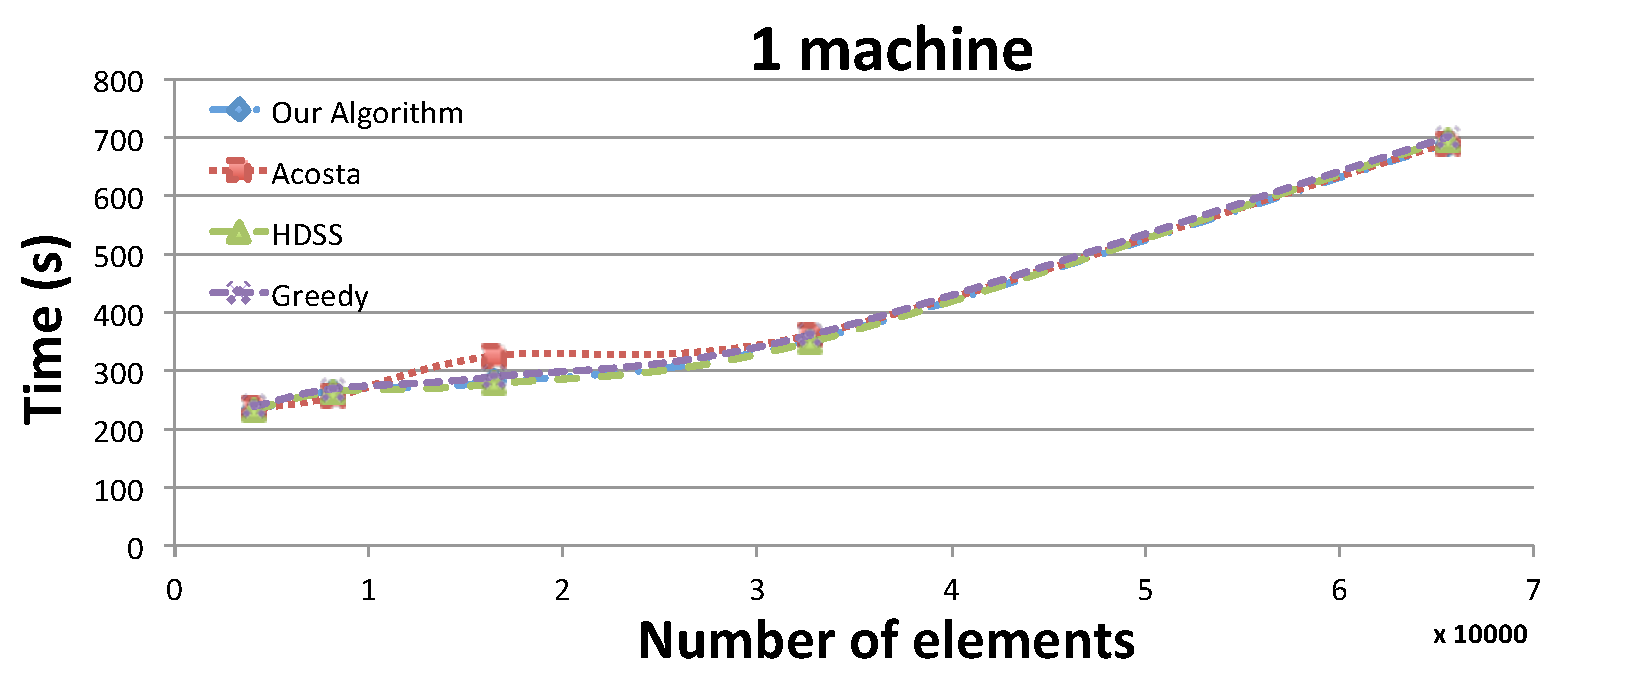
\includegraphics[scale=0.3]{1machine.pdf} \qquad
		%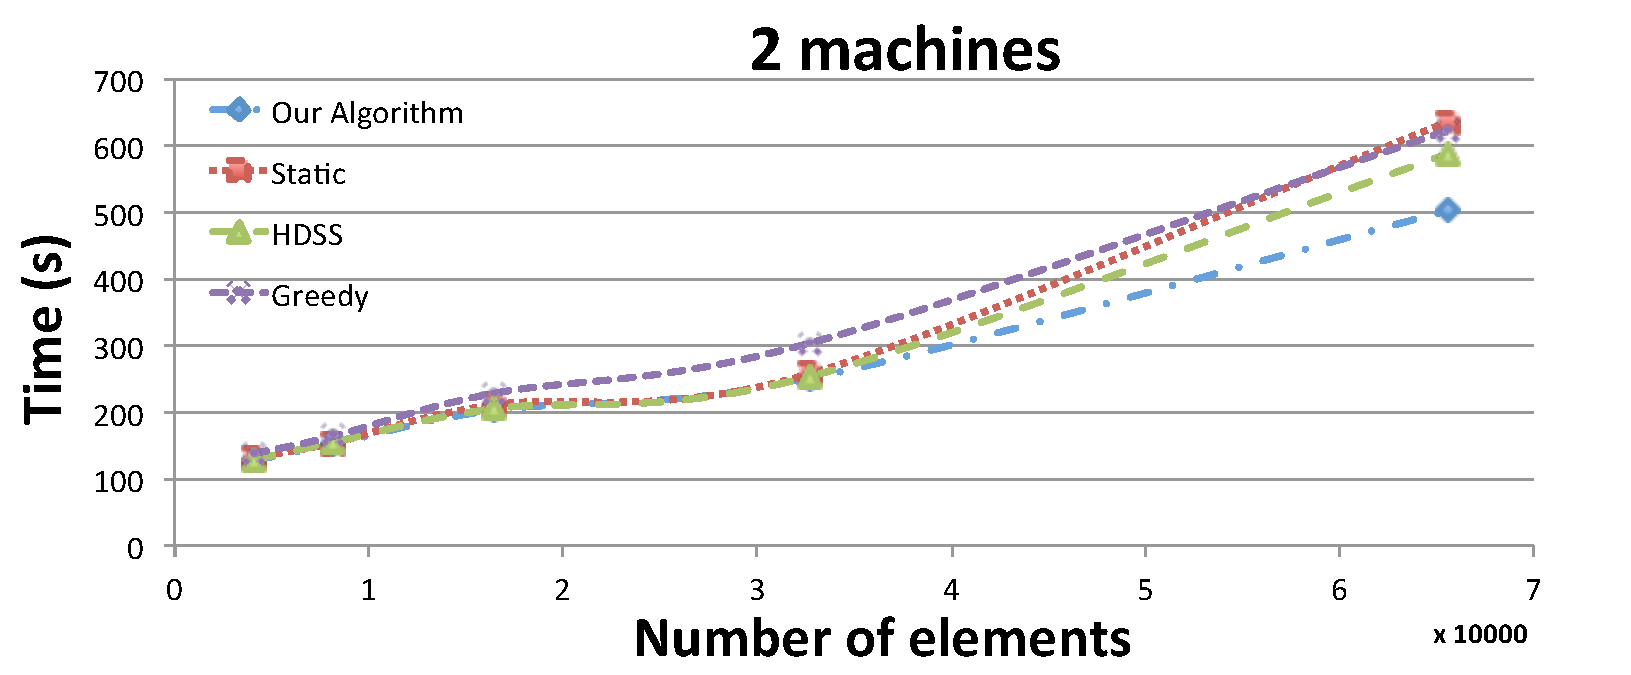
\includegraphics[scale=0.3]{2machines.pdf} \qquad
		%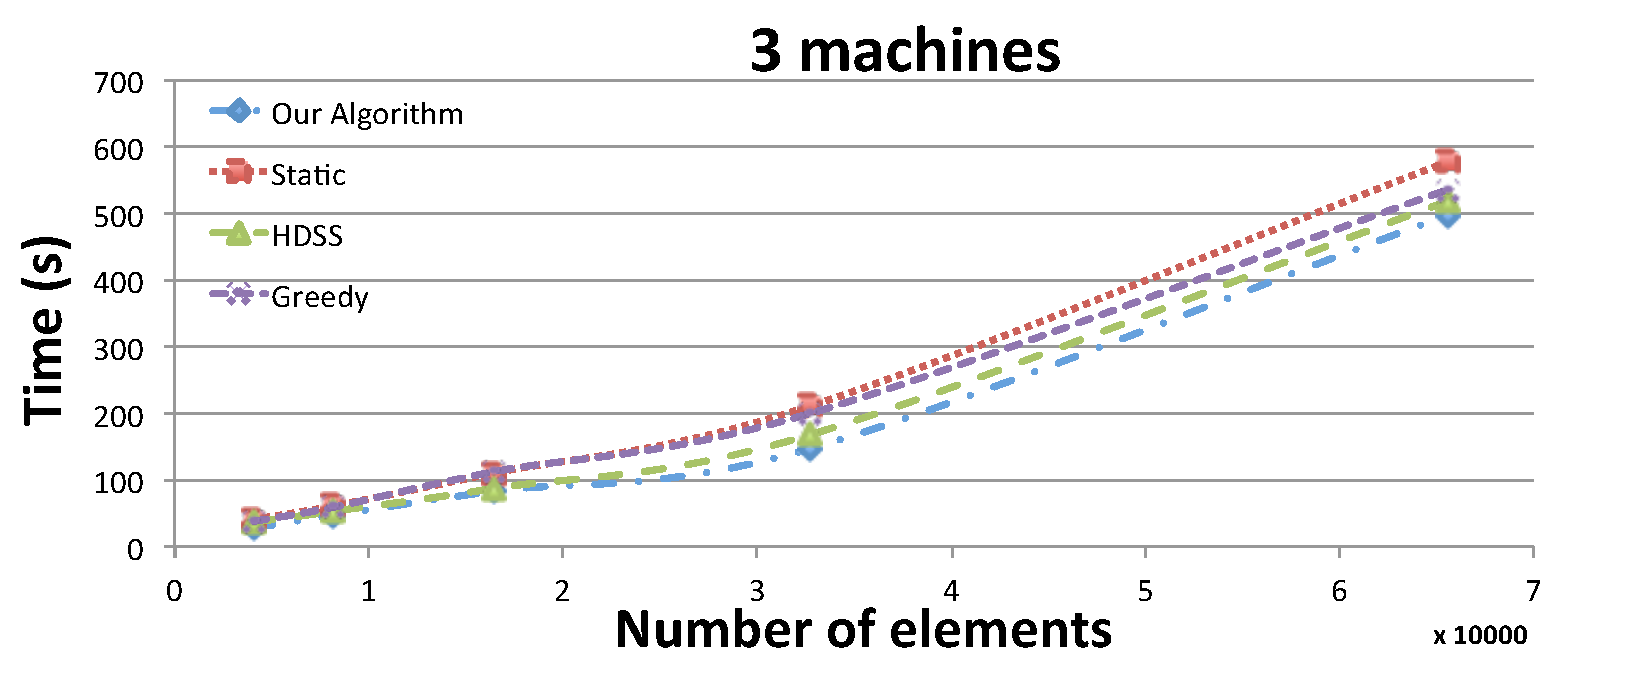
\includegraphics[scale=0.3]{3machines.pdf} \qquad
		%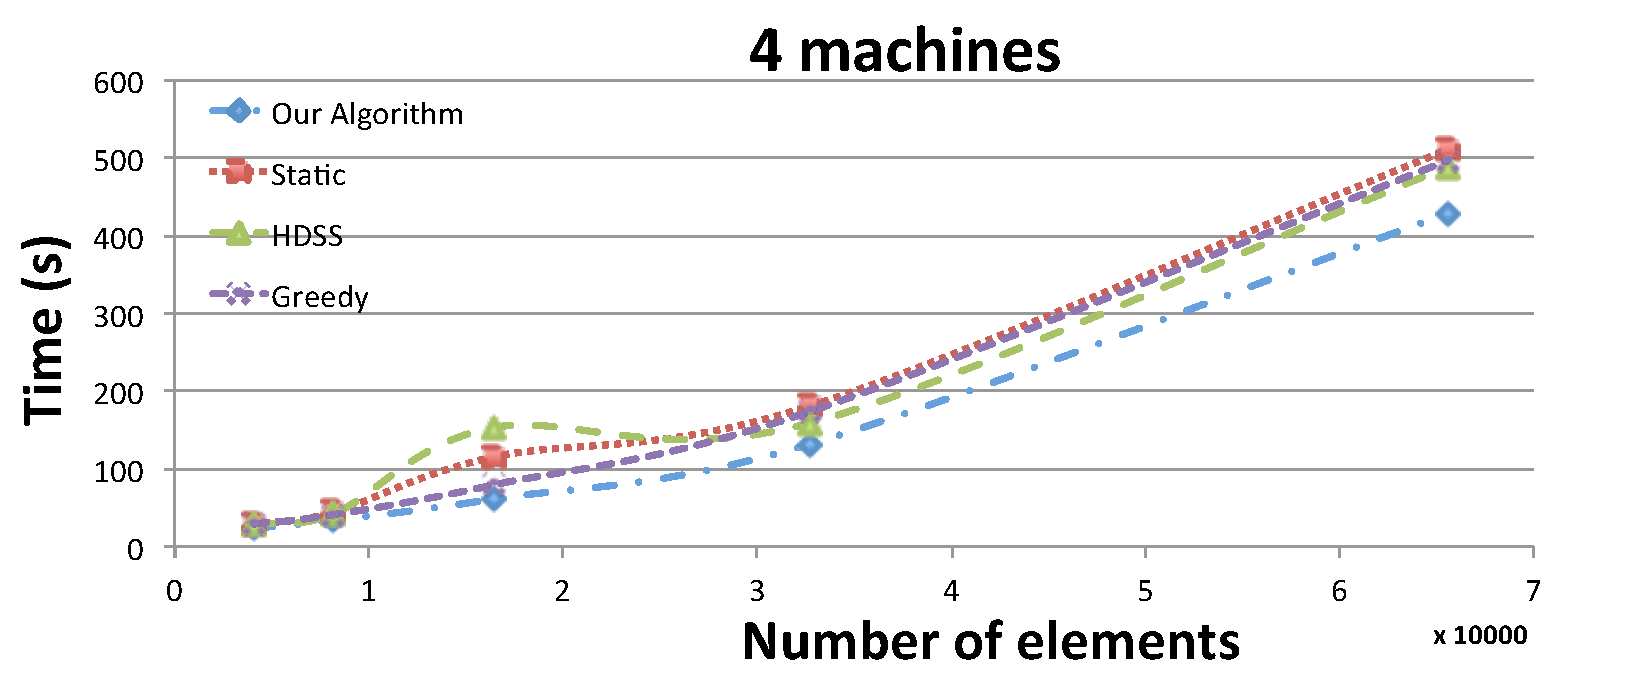
\includegraphics[scale=0.3]{4machines.pdf} 
	\caption{Execution time using different matrix sizes and number of
          machines with the matrix multiplication application.}
	\label{fig:todosJuntos}
	\end{center}
\end{figure*}



% RYC: Você rodou quantas vezes cada experimento? Qual o desvio padrão?
%10 vezes, desvio de 5.

\paragraph{Application execution time} Figure~\ref{fig:todosJuntos} shows the 
results obtained with matrices of sizes varying from $4096 \times 4096$ to $65536 \times
65536$ elements, for different number of machines. We present the average
execution time of 10 experiments, which resulted in small standard deviation
values, not shown in the graph for better visualization.

%between 4s and 5s.

With
only one machine the influence of the scheduling algorithm was small. The only choice that must be made is the selection between running on a 
CPU or GPU.
With more machines our algorithm achieves significantly better
results, since the number of GPU and CPUs types increases. Note that  the proposed algorithm perform better than the other algorithms on
all scenarios.

Table~\ref{table: comparativo} shows a more detailed comparison between the
proposed algorithm and the HDSS algorithm for smaller and larger matrix sizes. The
difference in execution time varies depending on the matrix size and number of
machines, but with 2 or more machines this difference was always above 9\% and up to
28\%. This variance in the difference can occur due to the variations in the
selection quality of task sizes in different configurations.

% RYC: Luis, veja se o parágrafo está certo, pois eu alterei seu conteúdo -> correto
%
% RYC: Aqui este tempo de 664 ms foi para quais cenários (tamanho de matriz e de
% máquinas)? O cenário foi adicionado.
We should also emphasize that the presented execution times include the time spent
calculating the size of the task sizes for each processor using the interior
point method. The mean time spent on this calculation was 664.9 ms, for the scenario with 4 machines and matrices of order 65536, with
standard deviation of 98.3 ms. Although not negligible, the gains obtained with
the better distribution of tasks sizes compensates the overhead caused by these calculations.

%For matrices with order 4096, the proposed algorithm used four machines during
%23.11 seconds, while the HDSS spent 29.91 seconds. Thus, in this case, our
%algorithm was 26.09\% faster. For matrices with order 65536, the proposed
%algorithm spent 428.01 seconds, while the HDSS 488.22; resulting, this, a
%improvement of 14.02\%.  The total cost of calculating the distribution of the
%blocks is 664.87 milliseconds, with standard deviation of 98.3 milliseconds. 

\begin{table*}[htb]
\centering
\caption{Matrix Multiplication execution times with HDSS and our algorithm}
\begin{scriptsize}
\begin{tabular}{c|c|c|c|c|c|c|}
\cline{2-7}
\multicolumn{1}{l|}{}                 & \multicolumn{3}{c|}{4096 elements}                              & \multicolumn{3}{c|}{65536 elements}                                                  \\ \hline
\multicolumn{1}{|l|}{Num. Machines} & HDSS (s) & Our algorithm (s) & \multicolumn{1}{l|}{Diff. (\%)} & \multicolumn{1}{l|}{HDSS (s)} & Our Algorithm (s) & \multicolumn{1}{l|}{Diff. (\%)} \\ \hline
\multicolumn{1}{|c|}{1 }       & 233     & 231              &   0.86                        
			 & 696                          &   689             &    1.01                        \\ \hline
\multicolumn{1}{|c|}{2 }      & 129     & 128              &    0.78                         
				& 587                         & 502             & 16.93                     \\ \hline
\multicolumn{1}{|c|}{3 }      & 36     & 28              & 28.57                            
			&          543                &    497           &      9.25                          \\ \hline
\multicolumn{1}{|c|}{4 }      & 29.91     & 23.11            & 26.09                       
			    & 488.22                          & 428.01              &     14.02            \\ \hline
\end{tabular}
\end{scriptsize}
\label{table: comparativo}
\end{table*}


\begin{table*}[htb]
\centering
\caption{Distribution of block sizes for Matrix Multiplication application}
\begin{scriptsize}
\begin{tabular}{|l|l|l|l|l|l|l|l|}
\cline{3-8}
\multicolumn{1}{l}{} &  & \multicolumn{2}{c|}{Acosta} & \multicolumn{2}{c|}{HDSS} & \multicolumn{2}{c|}{Our Algorithm} \\ 
\cline{3-8}
\multicolumn{1}{l}{} &  & \multicolumn{1}{c|}{4096 elements} & \multicolumn{1}{c|}{65536 elements} & \multicolumn{1}{c|}{4096 elements} & \multicolumn{1}{c|}{65536 elements} & \multicolumn{1}{c|}{4096 elements} & \multicolumn{1}{|c|}{65536 elements} \\ 
\cline{1-8}
\multicolumn{1}{|c}{} Machines &  & Size Ratio & Size Ratio & Size Ratio & Size Ratio & Size Ratio  & Size Ratio\\ 
\hline
A & CPU & \multicolumn{1}{c|}{$0.09 \pm 0.015$} & \multicolumn{1}{c|}{$0.05\pm 0.011$}  & \multicolumn{1}{c|}{$0.03 \pm 0.011$}  & \multicolumn{1}{c|}{$0.02 \pm 0.017$} & \multicolumn{1}{c|}{$0.04\pm 0.014$} & \multicolumn{1}{c|}{$0.01\pm 0.016$} \\ 
\cline{2-8}
 & GPU & \multicolumn{1}{c|}{$0.14 \pm 0.015$} & \multicolumn{1}{c|}{$0.12 \pm 0.011$} & \multicolumn{1}{c|}{$0.11 \pm 0.011$} & \multicolumn{1}{c|}{$0.13 \pm 0.017$} & \multicolumn{1}{c|}{$0.08 \pm 0.014$} & \multicolumn{1}{c|}{$0.12 \pm 0.016$} \\ 
\hline
B & CPU & \multicolumn{1}{c|}{$0.06 \pm 0.014$} & \multicolumn{1}{c|}{$0.06 \pm 0.012$} & \multicolumn{1}{c|}{$0.08 \pm 0.015$} & \multicolumn{1}{c|}{$0.08 \pm 0.017$} & \multicolumn{1}{c|}{$0.04 \pm 0.014$} & \multicolumn{1}{c|}{$0.01 \pm 0.017$} \\ 
\cline{2-8}
 & GPU & \multicolumn{1}{c|}{$0.13\pm 0.010$} & \multicolumn{1}{c|}{$0.14 \pm 0.011$} & \multicolumn{1}{c|}{$0.15\pm 0.015$} & \multicolumn{1}{c|}{$0.16 \pm 0.017$} & \multicolumn{1}{c|}{$0.12 \pm 0.015$} & \multicolumn{1}{c|}{$0.11 \pm 0.016$} \\ 
\hline
C & CPU & \multicolumn{1}{c|}{$0.12 \pm 0.013$} & \multicolumn{1}{c|}{$0.12 \pm 0.012$} & \multicolumn{1}{c|}{$0.08 \pm 0.017$} & \multicolumn{1}{c|}{$0.07 \pm 0.015$} & \multicolumn{1}{c|}{$0.04 \pm 0.014$} & \multicolumn{1}{c|}{$0.03 \pm 0.017$} \\ 
\cline{2-8}
 & GPU & \multicolumn{1}{c|}{$0.21 \pm 0.015$} & \multicolumn{1}{c|}{$0.21 \pm 0.011$} & \multicolumn{1}{c|}{$0.21 \pm 0.017$} & \multicolumn{1}{c|}{$0.21 \pm 0.015$} & \multicolumn{1}{c|}{$0.32 \pm 0.014$} & \multicolumn{1}{c|}{$0.35 \pm 0.016$} \\ 
\hline
D & CPU & \multicolumn{1}{c|}{$0.07 \pm 0.015$} & \multicolumn{1}{c|}{$0.08 \pm 0.011$} & \multicolumn{1}{c|}{$0.09 \pm 0.017$} & \multicolumn{1}{c|}{$0.09 \pm 0.015$} & \multicolumn{1}{c|}{$0.05 \pm 0.013$} & \multicolumn{1}{c|}{$0.04 \pm 0.017$} \\ 
\cline{2-8}
 & GPU & \multicolumn{1}{c|}{$0.18 \pm 0.015$} & \multicolumn{1}{c|}{$0.22 \pm 0.011$} & \multicolumn{1}{c|}{$0.25 \pm 0.017$} & \multicolumn{1}{c|}{$0.24 \pm 0.015$} & \multicolumn{1}{c|}{$0.31 \pm 0.013$} & \multicolumn{1}{c|}{$0.33 \pm 0.016$} \\ 
\hline
\end{tabular}
\end{scriptsize}
\label{table: comparativoBlocos}
\end{table*}

\paragraph{Block size distribution} Table~\ref{table: comparativoBlocos} shows 
the distribution of blocks among the machines for the three algorithms that try
to estimate block sizes: Acosta, HDSS and our algorithm. We was tested two
matrix sizes: $4096 \times 4096$ and $65536 \times 65536$. We used one thread
per CPU core and per GPU. We used the machines A, B, C and D, and one GPU per
machine. The values represent the amount of data allocated by each processor
from a normalized total size of 1, at the end of the performance modeling phase
for our algorithm, of phase 1 for HDSS algorithm, and of application execution
for Acosta algorithm. We performed 10 executions and present the average values
and standard deviations. The standard deviation values are small, showing that
all algorithms are stable through different executions.

When comparing the block size distributions generated by the three
load-balancing algorithms, we note that the same algorithm distribute similar
distributions for the two matrix sizes and that Acost and HDSS algorithms
produce similar distributions. When comparing to our algorithm, we can see that
it produces a qualitatively different distribution, with proportionally smaller
blocks allocated to CPUs and larger blocks to GPUs from machines C and D, which
contain the largest number of cores. This difference occurs because HDSS and
Acost algorithm use simple linear weighted means from a set of performance
coefficients, one per processor. Our algorithm uses the complete performance
curve of each processor and solves the resulting system of equations, resulting
in more precise estimates of the better block division scheme.

%The greedy algorithm does not directly use information on the processing speeds
%of the devices and simply provides the tasks to free processors and the
%differences in finish times was larger than for our algorithm and HDSS. But was
%better than the static one, where incorrect predictions are maintained during
%the entire execution. HDSS uses the beginning of the execution to estimate the
%best block size distribution and uses this distribution through the complete
%execution. Its cruder approximation generate larger unbalances between the
%threads than our algorithm, which is reflected in the difference in the
%finishing time between the threads.

% RYC: Na sua simulações houve alguma reconfiguração devido à ultrapassagem do limiar?
% Sim, em alguns casos, mas foi considerado a média dos casos.
%Our algorithm obtained the most accurate data distribution estimation, solving
%an optimization problem with the restriction that all units should finish the
%execution of the tasks at the same time. Also, in the instances where the
%selected distribution had an unbalance above a threshold, it was rebalanced by
%the algorithm.


\begin{table*}[htb]
\centering
\caption{Idle processor times for Matrix Multiplication application}
\begin{scriptsize}
\begin{tabular}{|l|l|l|l|l|l|}
\cline{3-6}
\multicolumn{1}{l}{} &  & \multicolumn{2}{c|}{HDSS} & \multicolumn{2}{c|}{Our Algorithm} \\ 
\cline{3-6}
\multicolumn{1}{l}{} &  & \multicolumn{1}{c|}{4096 elements} & \multicolumn{1}{c|}{65536 elements} & \multicolumn{1}{c|}{4096 elements} & \multicolumn{1}{c|}{65536 elements} \\ 
\cline{1-6}
\multicolumn{1}{|c}{} Machines &  & Idle Time (s) & Idle Time (s) & Idle Time (s) & Idle Time (s) \\ 
\hline
A & CPU & \multicolumn{1}{c|}{$1.32 \pm 0.21$} & \multicolumn{1}{c|}{$8.32  \pm 0.92$} & \multicolumn{1}{c|}{$0.62  \pm 0.10$} & \multicolumn{1}{c|}{$1.23 \pm 0.14$} \\ 
\cline{2-6}
 & GPU & \multicolumn{1}{c|}{$1.16 \pm 0.21$} & \multicolumn{1}{c|}{$7.43 \pm 0.90$} & \multicolumn{1}{c|}{$0.92 \pm 0.11$} & \multicolumn{1}{c|}{$1.67 \pm 0.15$} \\ 
\hline
B & CPU & \multicolumn{1}{c|}{$1.41 \pm 0.21$} & \multicolumn{1}{c|}{$6.32 \pm 0.91$} & \multicolumn{1}{c|}{$0.78 \pm 0.11$} & \multicolumn{1}{c|}{$1.88 \pm0.16$} \\ 
\cline{2-6}
 & GPU & \multicolumn{1}{c|}{$1.33 \pm 0.20$} & \multicolumn{1}{c|}{$6.82 \pm 0.91$} & \multicolumn{1}{c|}{$0.86 \pm 0.10$} & \multicolumn{1}{c|}{$1.99 \pm 0.16$} \\ 
\hline
C & CPU & \multicolumn{1}{c|}{$1.68 \pm 0.21$} & \multicolumn{1}{c|}{$7.76 \pm 0.91$} & \multicolumn{1}{c|}{$0.44 \pm 0.08$} & \multicolumn{1}{c|}{$1.54 \pm 0.16$} \\ 
\cline{2-6}
 & GPU & \multicolumn{1}{c|}{$1.41 \pm 0.21$} & \multicolumn{1}{c|}{$9.98 \pm 0.93$} & \multicolumn{1}{c|}{$0.45 \pm 0.11$} & \multicolumn{1}{c|}{$1.34 \pm 0.15$} \\ 
\hline
D & CPU & \multicolumn{1}{c|}{$1.72 \pm 0.25$} & \multicolumn{1}{c|}{$7.43 \pm 0.92$} & \multicolumn{1}{c|}{$0.93 \pm 0.11$} & \multicolumn{1}{c|}{$1.31 \pm 0.14$} \\ 
\cline{2-6}
 & GPU & \multicolumn{1}{c|}{$1.32 \pm 0.2$} & \multicolumn{1}{c|}{$9.97 \pm 0.93$} & \multicolumn{1}{c|}{$0.74 \pm 0.11$} & \multicolumn{1}{c|}{$1.45 \pm 0.15$} \\ 
\hline
\end{tabular}
\end{scriptsize}
\label{table: ociosoBlocos}
\end{table*}

\paragraph{Processor Idleness} Table~\ref{table: ociosoBlocos} shows the amount of time each CPU and GPU was
idle during application execution for our and HDSS algorithms, which resulted in
the best application execution times. We used the same experimental
configuration from Table~\ref{table: comparativoBlocos}. The table represents the ratio of blocks received by each processor, CPU or GPU. At each step of the submission of the tasks we recorded the size of the block sent to each processor. We ran each algorithm 10 times, and perform the calculation of the average block sent to each processor.
Acosta algorithm (not
shown) produces significantly larger idleness, since it synchronizes the block
executions multiple times until it reaches an equilibrium.

The idleness occur mainly in the first phase of the algorithm, where
non-optimal block sizes are used to estimate the computational capabilities of
each processor. Our algorithm starts to adapt the block sizes in this phase
(Figure~\ref{fig: algoritmo}), causing a reduction in the generated idleness. 

There can also be additional idleness in the end of application. HDSS prevents
part of this idleness using decreasing block size values during application
execution. If some processor is idle at the end, it can receive extra small
blocks to process. Our algorithm perform the re-balancing process when the
difference in execution time is above a threshold. 


%\begin{figure}[htb]
%	\begin{center}
%	\centering
%			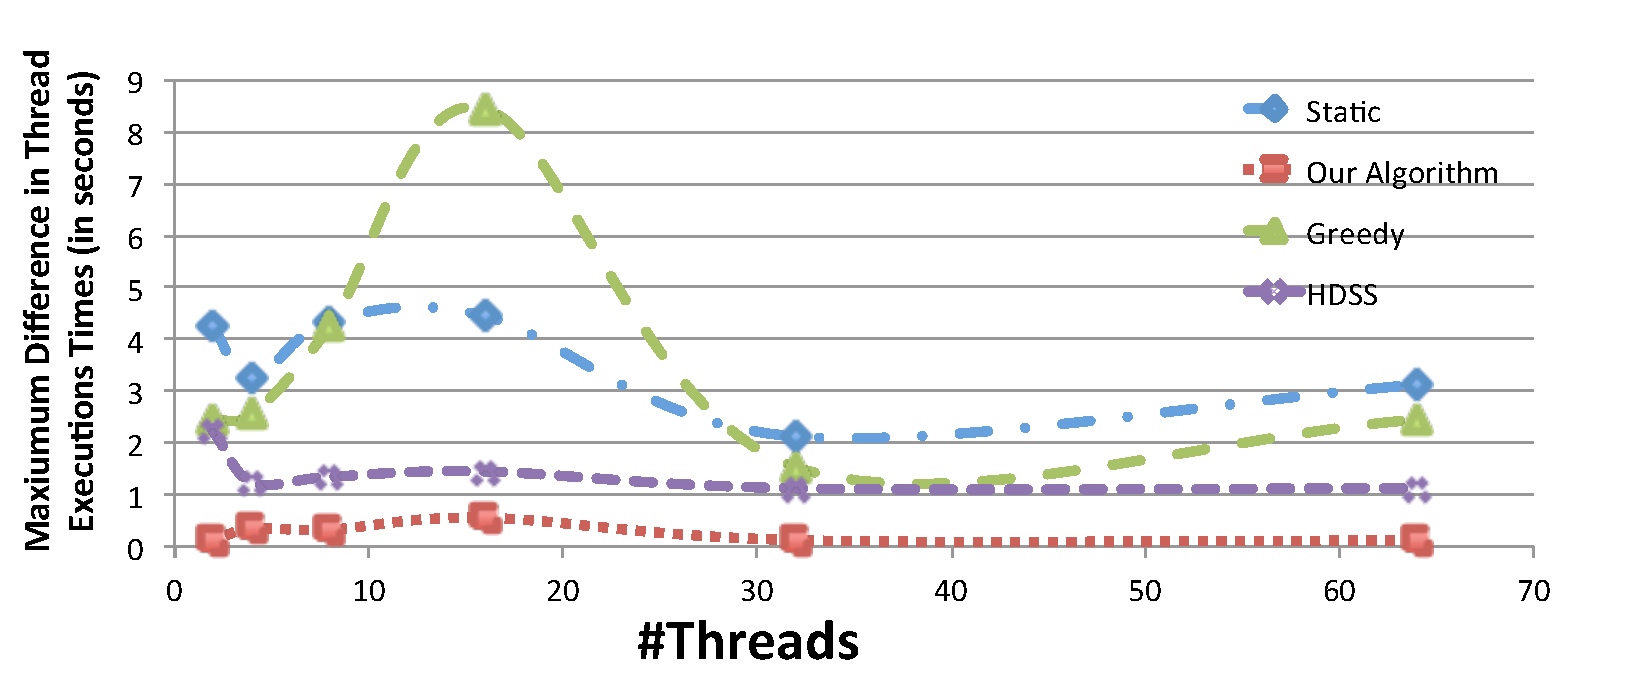
\includegraphics[scale=0.33]{MaximoDiferenca_matrix_novo.pdf}
%	\caption{Time differences between the earliest and latest finishing
 %         threads with the matrix multiplication algorithm and four machines.}
%	\label{fig:diferencaThreads}
%	\end{center}
%\end{figure}
% RYC: cada figura com os tempos finais das threads está com um tamanho diferente -> OK

% RYC: retirar os títulos dos gráficos -> Retirado de alguns. 

% RYC: aqui não está muito claro também. Precisa explicar o que são essas
% threads (1 a 60), como elas são distribuídas entre as máquinas e por que este
% experimento foi realizado. 
%	
% RYC: Além disso, o que são estes earliest and latest finishing tasks? Por que
% pegar só as threads no final? %Existem barreiras de sincronização nos
% algoritmos?  
%Nestes casos, não seria melhor medir os atrasos em cada barreira
% de sincronização?
%Nao existe barreira de sincronizaçao nos algoritmos, por isso a comparacao é justa. O que pode ocorrer sincronizacão é o nosso, mas aqui eu tirei o teste de sincronizacao, apenas para comparar o atraso no fim das threads. 

%To better understand these results, we evaluated the time difference between the
%earliest and latest finishing threads, in the scenario with four machines and
%matrices with size $65535 \times 65535$.  Figure~\ref{fig:diferencaThreads}
%shows the results for different number of threads for each algorithm. The
%threads were distributed equally among machines, including threads on the GPU
%and CPU. For two threads we used only the CPUs. In the y axis, we presented the
%maximum difference between the end of the performances of each algorithm for the
%same scenario in only execution. Our algorithm have the smallest amount of difference among all
%the algorithms implying a better load balance among processors. Other algorithms
%show considerable differences mostly because of idle GPUs at the end of
%executions.

% DC: "There are big differences among end of threads." Quais?! Escrevi errado.
%The greedy algorithm does not directly use information on the processing speeds
%of the devices and simply provides the tasks to free processors and the
%differences in finish times was larger than for our algorithm and HDSS. But was
%better than the static one, where incorrect predictions are maintained during
%the entire execution. HDSS uses the beginning of the execution to estimate the
%best block size distribution and uses this distribution through the complete
%execution. Its cruder approximation generate larger unbalances between the
%threads than our algorithm, which is reflected in the difference in the
%finishing time between the threads.

% RYC: Na sua simulações houve alguma reconfiguração devido à ultrapassagem do limiar?
% Sim, em alguns casos, mas foi considerado a média dos casos.
%Our algorithm obtained the most accurate data distribution estimation, solving
%an optimization problem with the restriction that all units should finish the
%execution of the tasks at the same time. Also, in the instances where the
%selected distribution had an unbalance above a threshold, it was rebalanced by
%the algorithm.

%------------------------------------------------------------------------------------------------
\subsection{Blackscholes}

\begin{figure*}[htb]
	\begin{center}
	\centering
			%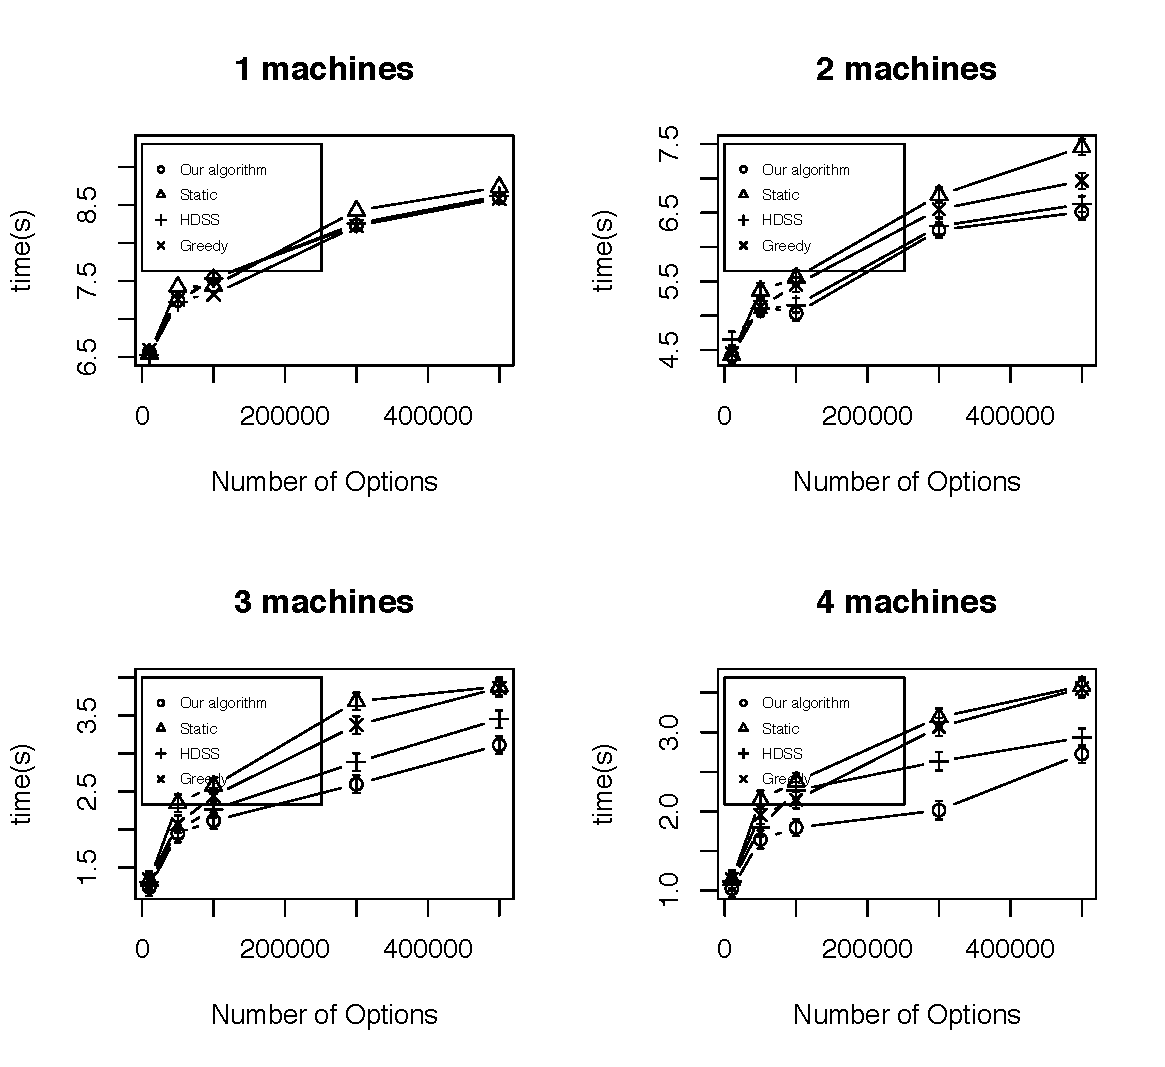
\includegraphics[scale=0.45]{BlackScholes4MachinesNOVO.pdf}
		%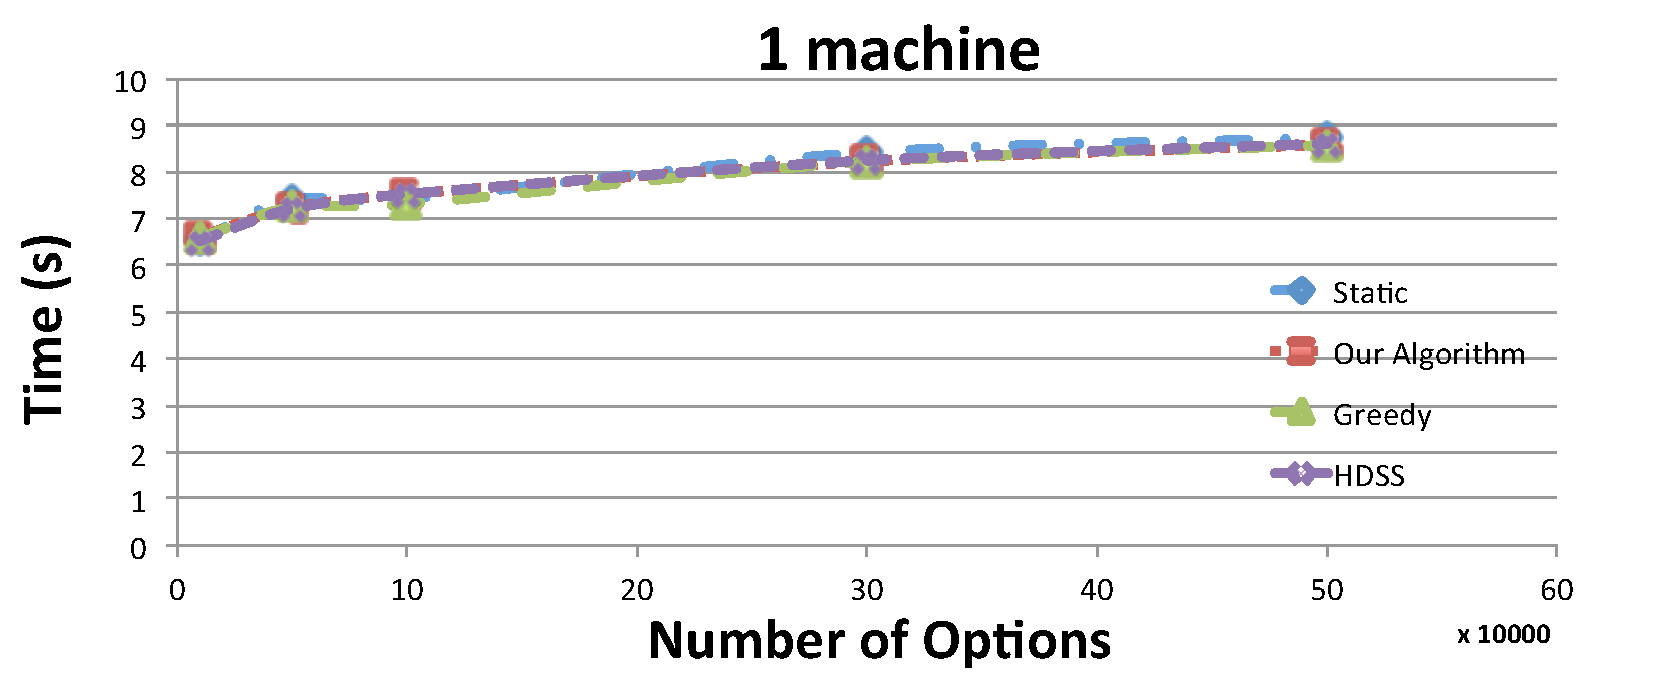
\includegraphics[scale=0.3]{1machineBlack.pdf} \quad
		%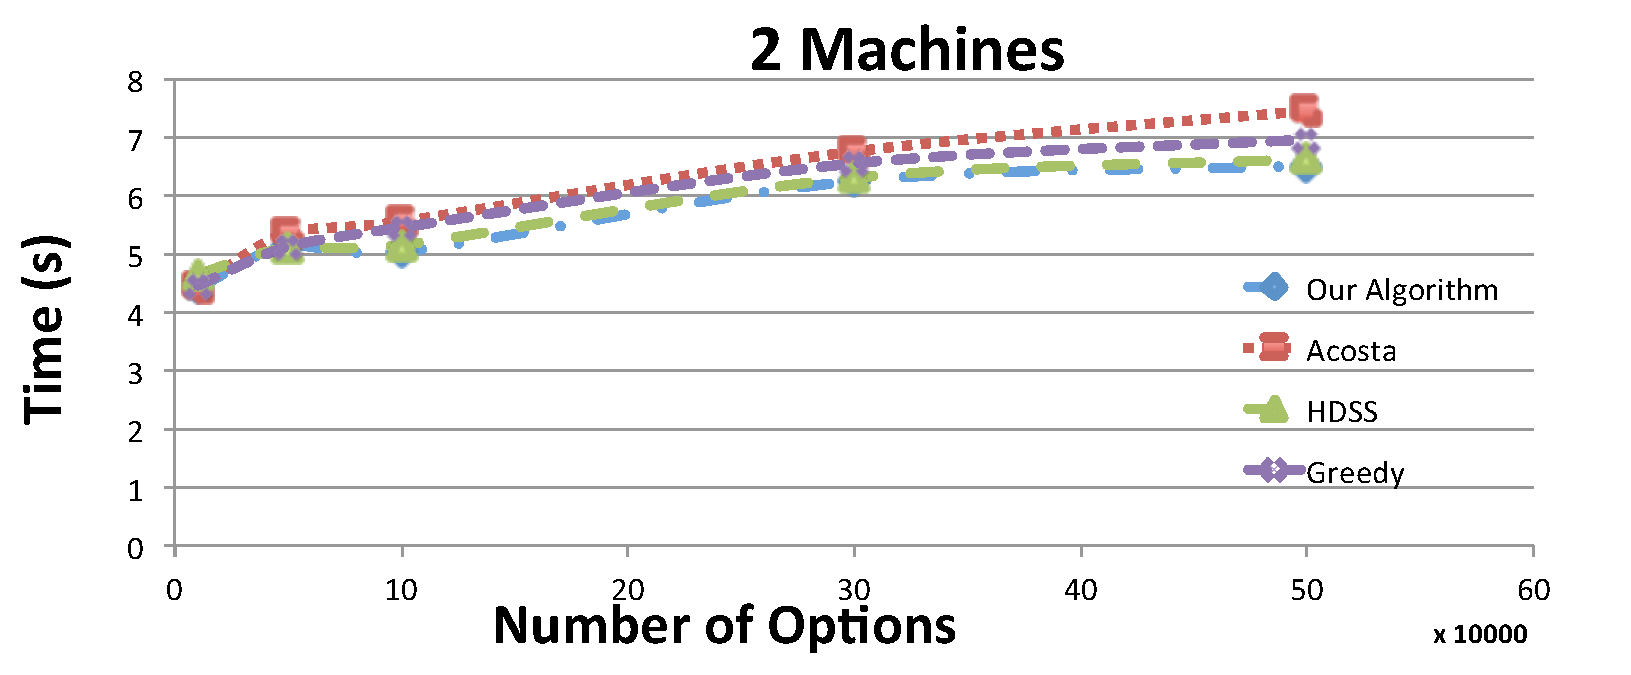
\includegraphics[scale=0.3]{2machineBlack.pdf} \quad
		%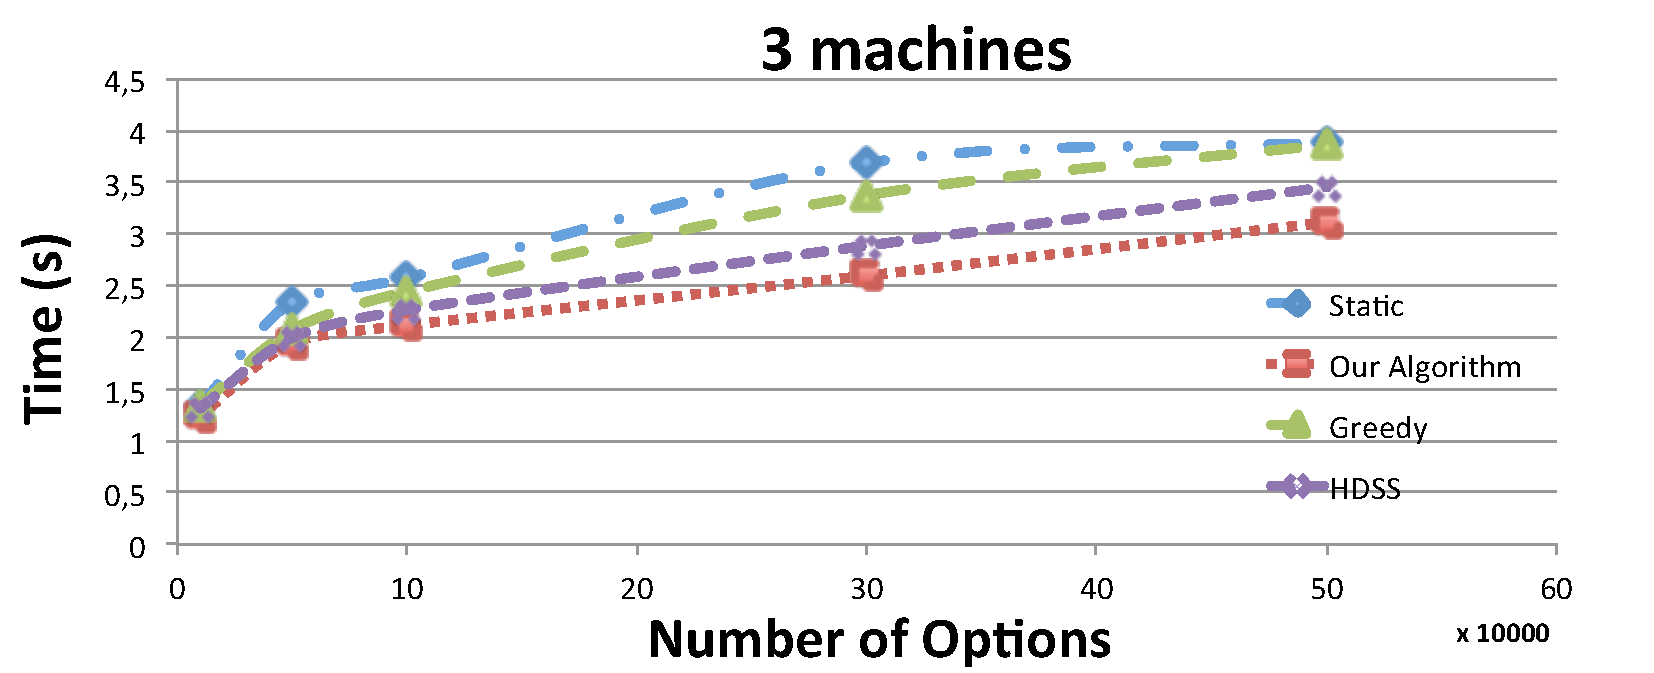
\includegraphics[scale=0.3]{3machineBlack.pdf} \quad
		%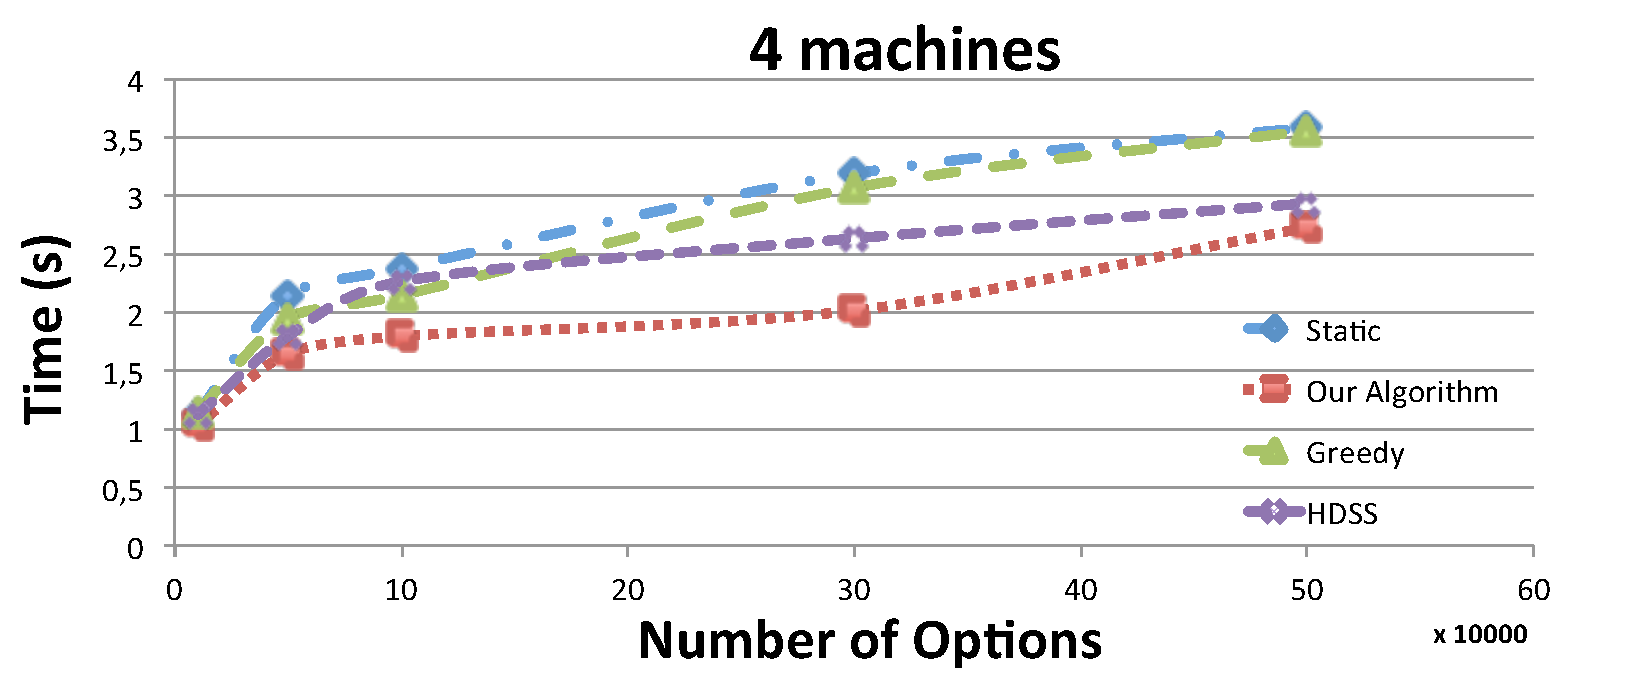
\includegraphics[scale=0.3]{4machineBlack.pdf} 

		\subfigure[1 machine]{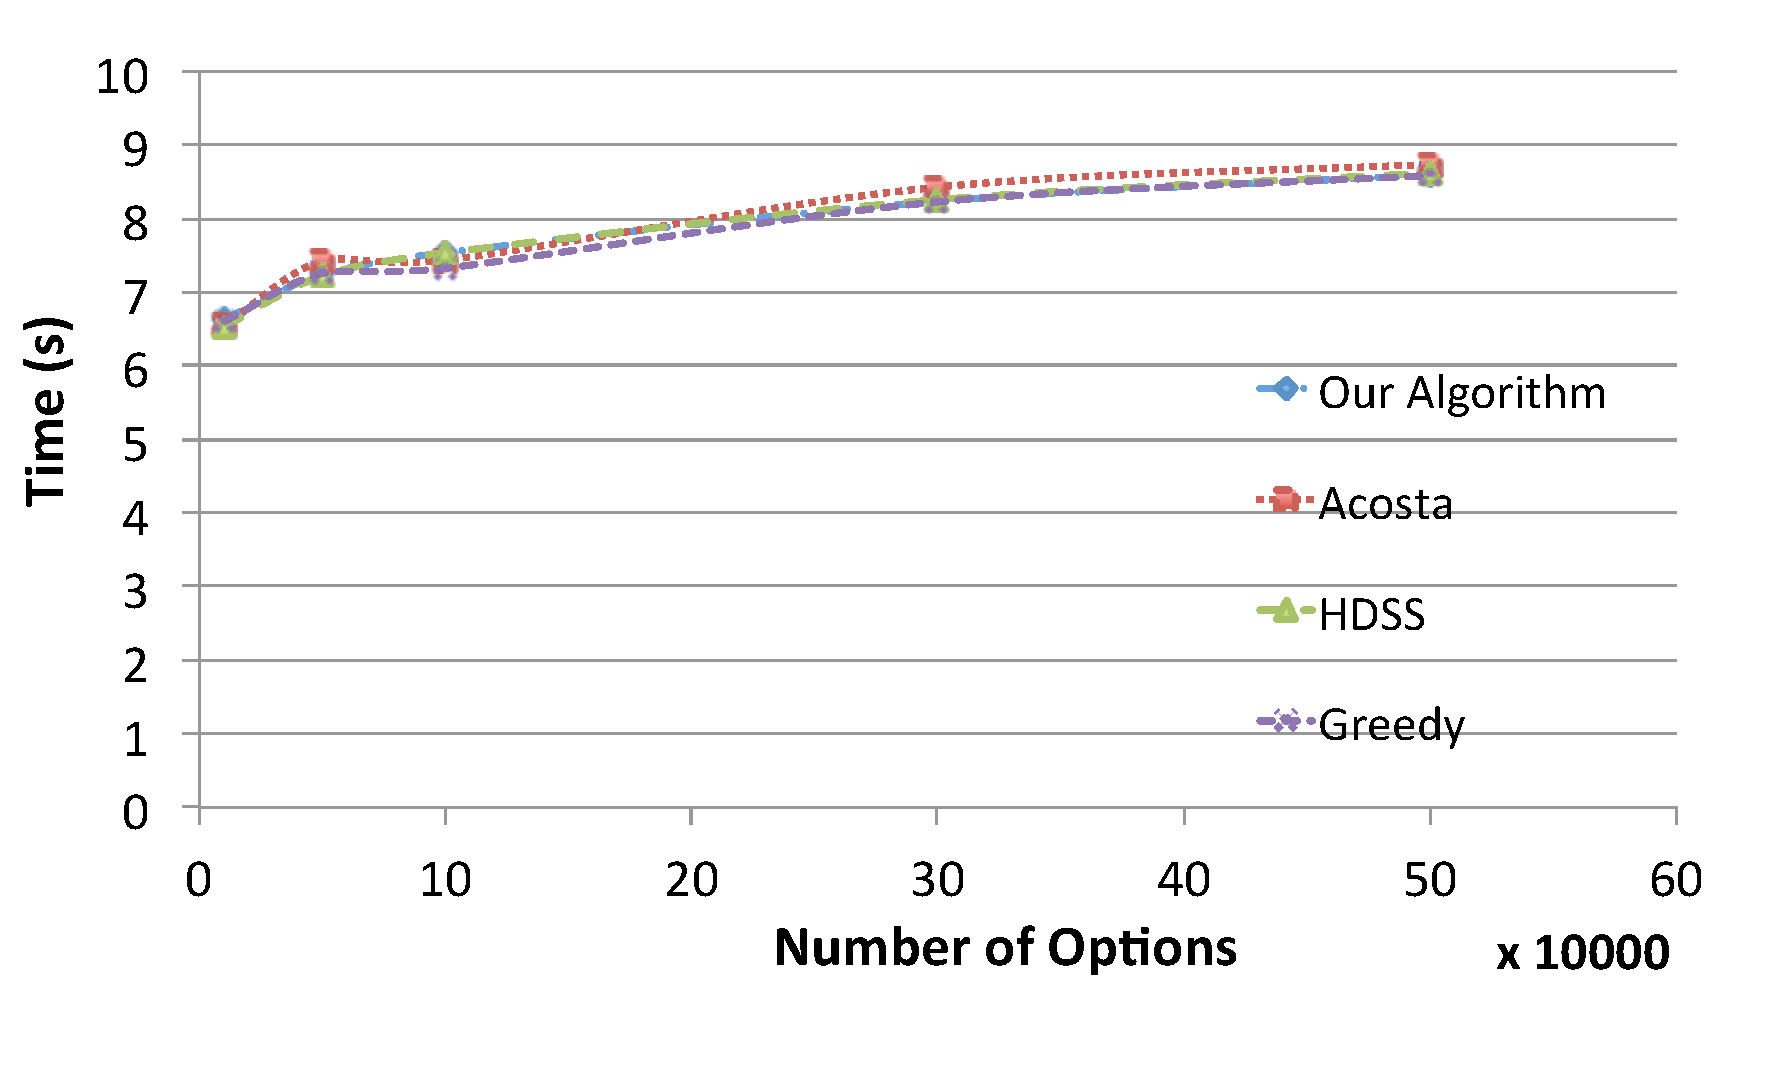
\includegraphics[height=3.3cm, width=4.52cm]{1machineBlackN.pdf}}
	        \subfigure[2 machine]{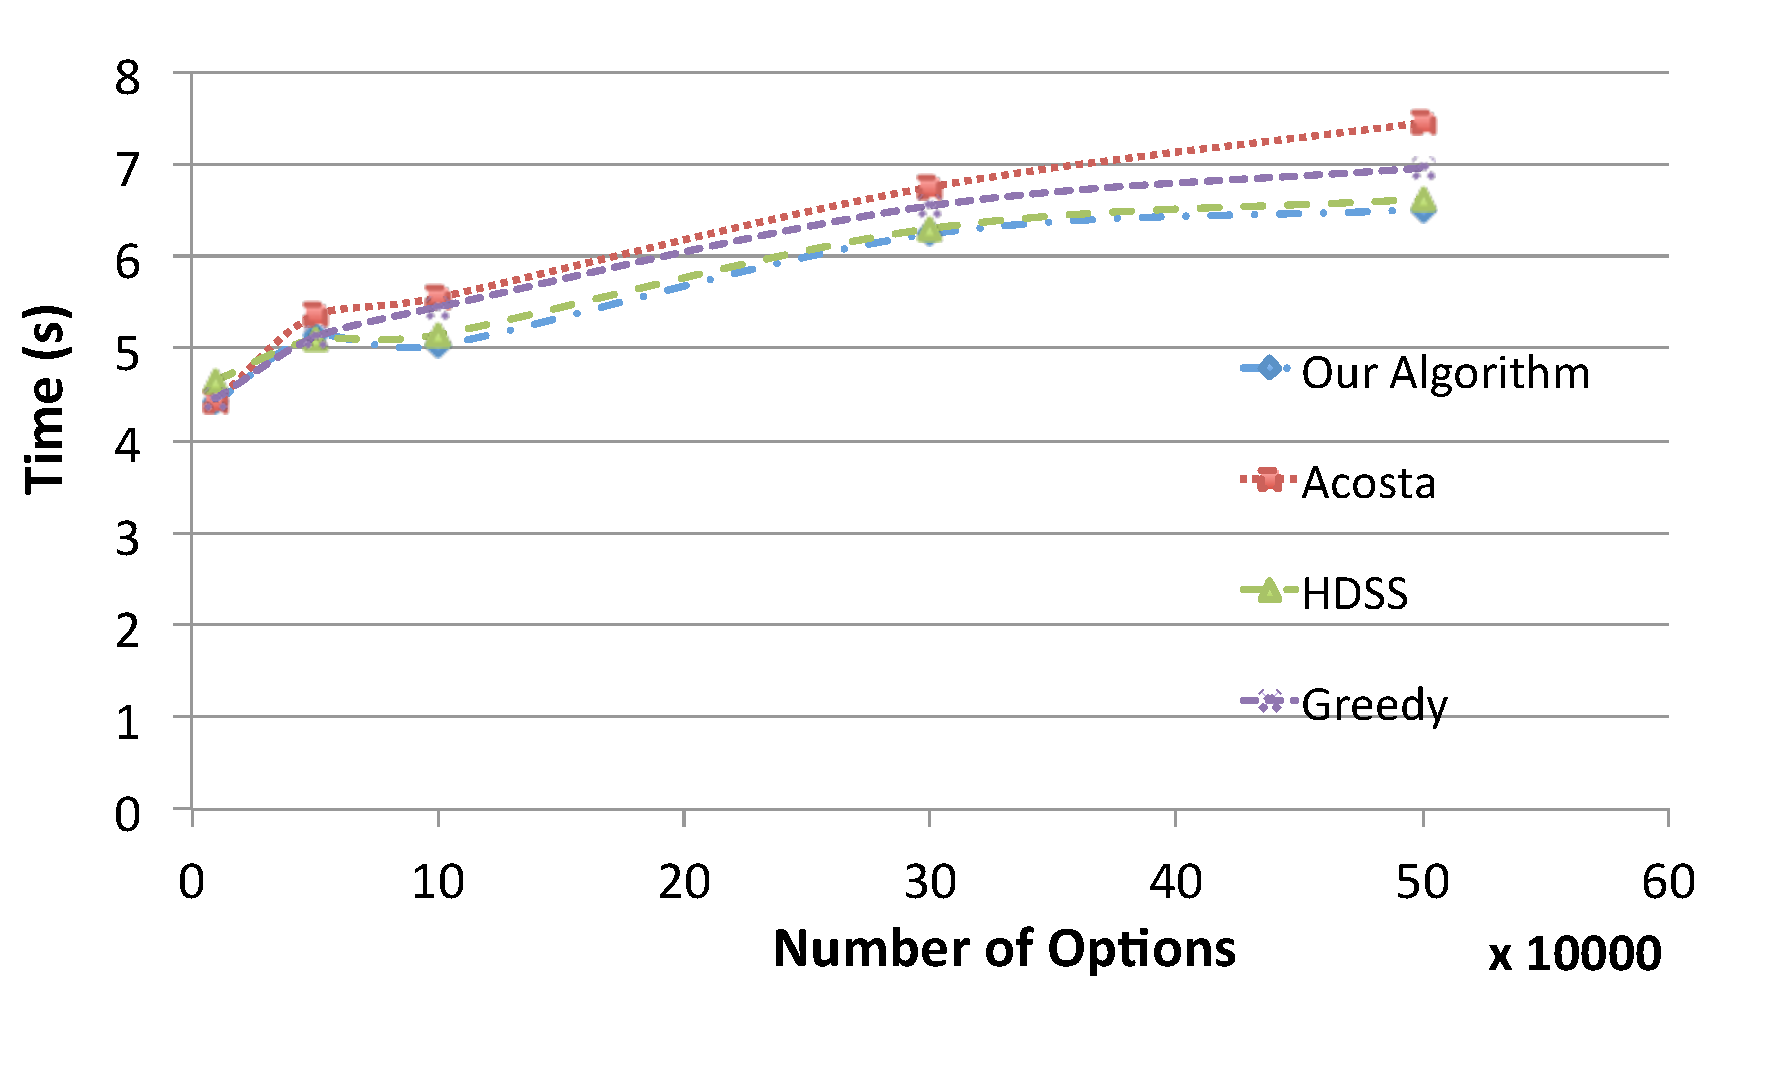
\includegraphics[height=3.3cm, width=4.52cm]{2machineBlackN.pdf}}
		\subfigure[3 machine]{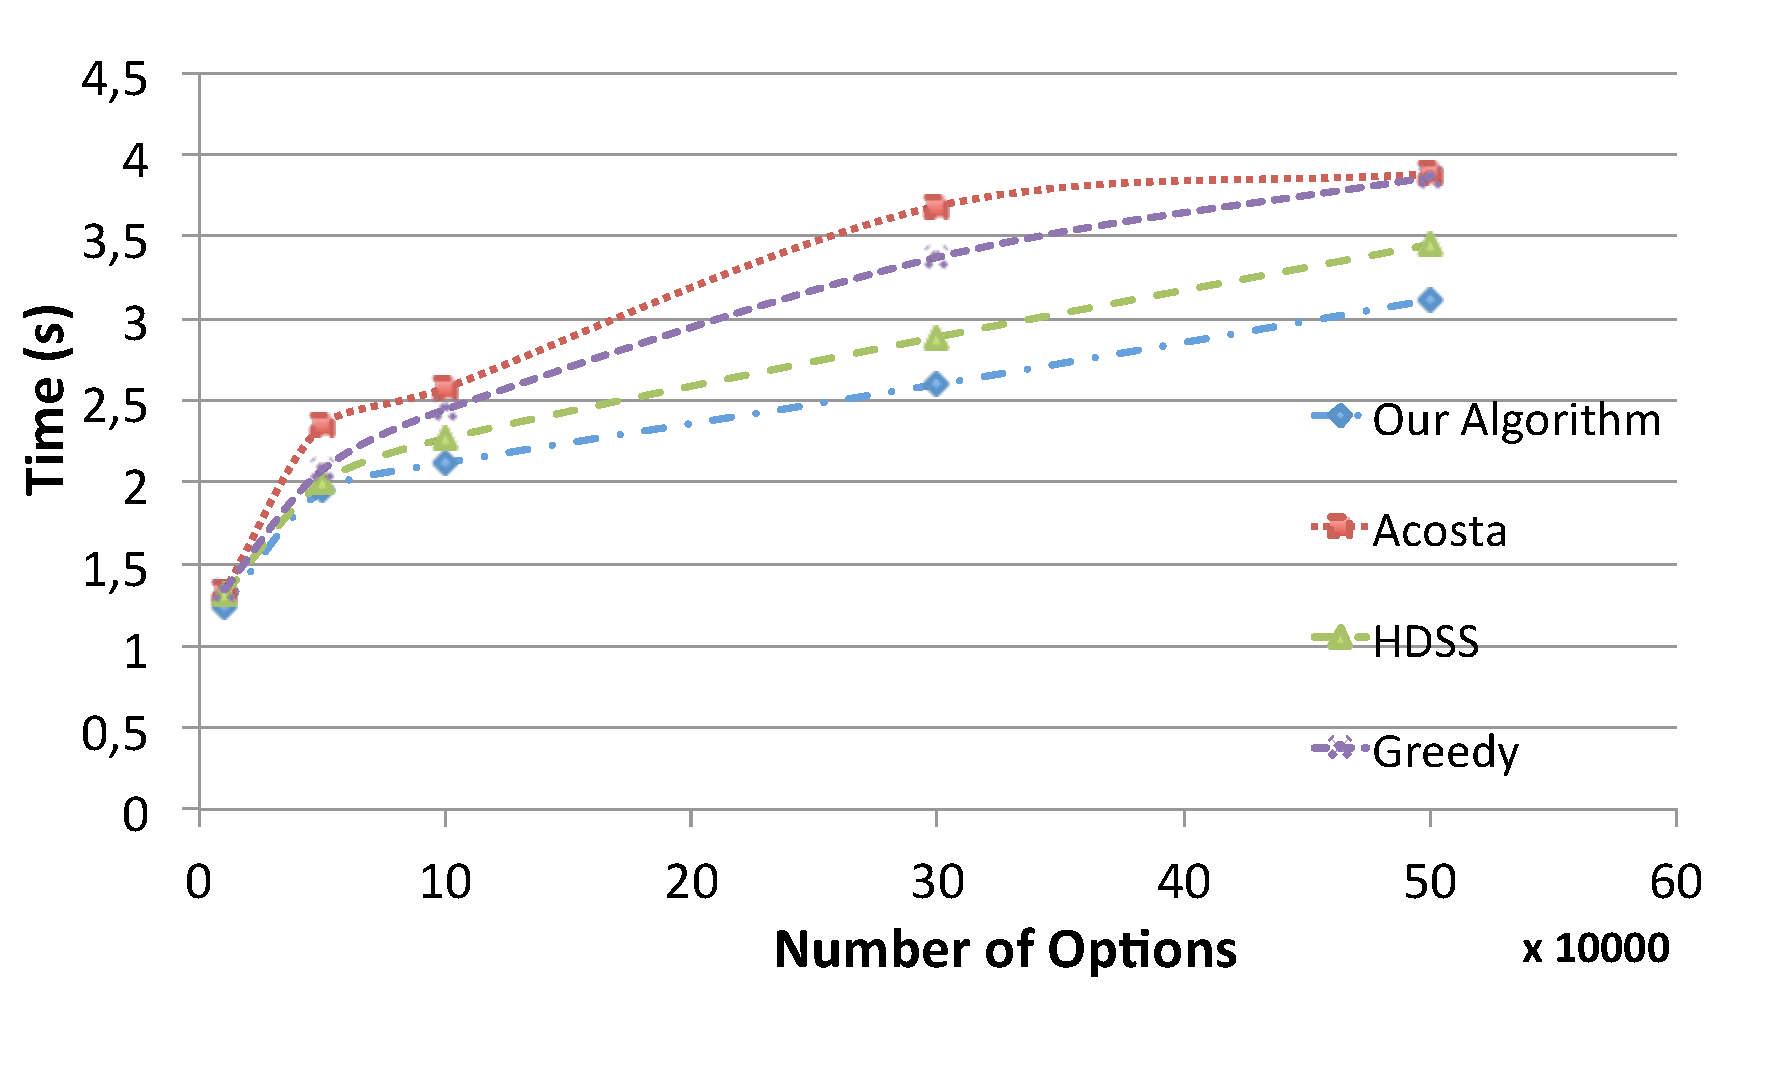
\includegraphics[height=3.3cm, width=4.52cm]{3machineBlackN.pdf}}
		\subfigure[4 machine]{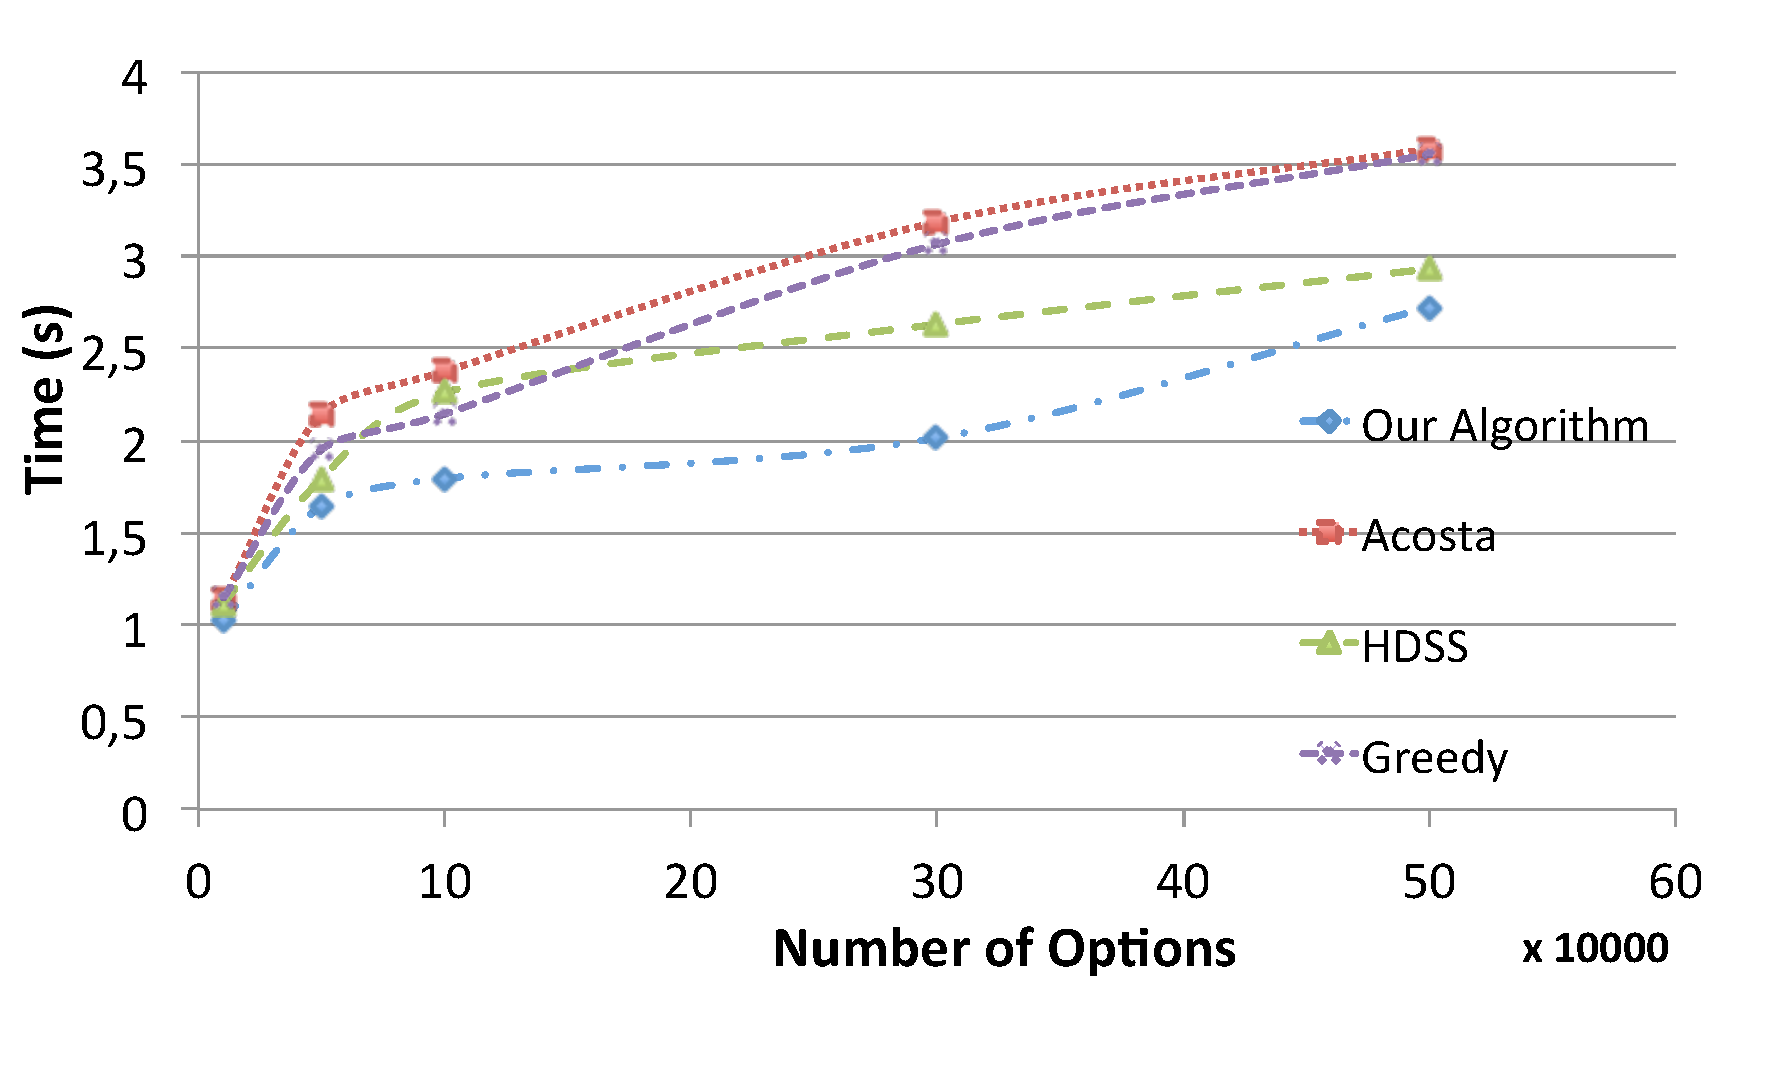
\includegraphics[height=3.3cm, width=4.52cm]{4machineBlackN.pdf}}
	\caption{Difference in runtime with different number options}
	\label{fig:black}
	\end{center}
\end{figure*}

We evaluate the execution time of the \emph{Blackscholes} application using
different number of machines and load-balancing algorithms, for different number
of stock options. Figure~\ref{fig:black} shows that performance differences were
larger in more heterogeneous environments. This application has linear
complexity in relation to the number of options, showing that our scheduling
algorithm is also useful with this class of applications. Our algorithm was
configured with a threshold of 10\% of the execution time and initial block size
of 2048 elements. The initial block size of HDSS algorithm was 1024 elements.

Table~\ref{table: black} compares the execution times of our algorithm and HDSS,
for the execution with 10,000 and 500,000 options. The largest difference
occurred with three and four machines, with values between 5\% and 11\%. The
mean overhead of our algorithm to determine the distribution of block sizes, for
4 machines and 500,000 options was 201.32ms, with standard deviation of 0.34ms.
Although not negligible, the best distribution of tasks sizes found compensates
this overhead.


% RYC: Aqui este tempo de 201 ms foi para quais cenários (número de opções e de
% máquinas)? Para o caso em que a aplicação executou em 1 segundo não está
% grande demais? Por que deu diferente da multiplicação de matrizes?

%Aparentemente está grande, mas devido ao comportamento linear do algoritmo, a parte que gera a aproximação por mínimos quadrados realiza de forma mais rápida, pois testa de primeira as equações lineares, e a solução do sistema se torna simples (todas lineares).


\begin{table*}[htb]
\centering
\caption{Blackscholes application execution times with HDSS and our algorithm}
\begin{scriptsize}
\begin{tabular}{c|c|c|c|c|c|c|}
\cline{2-7}
\multicolumn{1}{l|}{}                 & \multicolumn{3}{c|}{10,000 Options}                              & \multicolumn{3}{c|}{500,000 Options}                                                  \\ \hline
\multicolumn{1}{|l|}{Num. Machines} & HDSS (s) & Our algorithm (s) & \multicolumn{1}{l|}{Diff. (\%)} & \multicolumn{1}{l|}{HDSS (s)} & Our algorithm (s) & \multicolumn{1}{l|}{Diff. (\%)} \\ \hline
\multicolumn{1}{|c|}{1 }       & 6.52     & 6.56              &    -0.61                       
			 & 8.61                          & 8.59              &   0.23                         \\ \hline
\multicolumn{1}{|c|}{2 }      & 4.65     & 4.41              &    5.44                         
				& 6.62                          & 6.51              & 1.68                            \\ \hline
\multicolumn{1}{|c|}{3 }      & 1.31     & 1.24              & 5.56                            
			& 3.45                          & 3.11              &         10.93                    \\ \hline
\multicolumn{1}{|c|}{4 }      & 1.11     & 1.02              & 8.82                       
			    & 2.93                          & 2.72              &         7.72                  \\ \hline
\end{tabular}
\end{scriptsize}
\label{table: black}
\end{table*}

\begin{table*}[htb]
\centering
\caption{Distribution of block sizes for Blackscholes application}
\begin{scriptsize}
\begin{tabular}{|l|l|l|l|l|l|l|l|}
\cline{3-8}
\multicolumn{1}{l}{} &  & \multicolumn{2}{c|}{Acosta} & \multicolumn{2}{c|}{HDSS} & \multicolumn{2}{c|}{Our Algorithm} \\ 
\cline{3-8}
\multicolumn{1}{l}{} &  & \multicolumn{1}{c|}{10,000 opt} & \multicolumn{1}{c|}{500,000 opt} & \multicolumn{1}{c|}{10,000 opt} & \multicolumn{1}{c|}{500,000 opt} & \multicolumn{1}{c|}{500,000 opt} & \multicolumn{1}{c|}{500,000 opt} \\ 
\cline{1-8}
\multicolumn{1}{|c}{} Machine &  & Size Ratio & Size Ratio & Size Ratio & Size Ratio & Size Ratio & Size Ratio \\ 
\hline
A & CPU & \multicolumn{1}{c|}{$0.07 \pm 0.015$} & \multicolumn{1}{c|}{$0.06 \pm 0.011$} & \multicolumn{1}{c|}{$0.06 \pm 0.011$} & \multicolumn{1}{c|}{$0.06 \pm 0.017$} & \multicolumn{1}{c|}{$0.02 \pm 0.014$} & \multicolumn{1}{c|}{$0.01 \pm 0.016$} \\ 
\cline{2-8}
 & GPU & \multicolumn{1}{c|}{$0.13 \pm 0.015$} & \multicolumn{1}{c|}{$0.16 \pm 0.011$} & \multicolumn{1}{c|}{$0.15  \pm 0.011$} & \multicolumn{1}{c|}{$0.17  \pm 0.017$} & \multicolumn{1}{c|}{$0.03  \pm 0.014$} & \multicolumn{1}{c|}{$0.07  \pm 0.016$} \\ 
\hline
B & CPU & \multicolumn{1}{c|}{$0.06 \pm 0.014$} & \multicolumn{1}{c|}{$0.06  \pm 0.012$} & \multicolumn{1}{c|}{$0.08 \pm 0.015$} & \multicolumn{1}{c|}{$0.08 \pm 0.017$} & \multicolumn{1}{c|}{$0.02 \pm 0.014$} & \multicolumn{1}{c|}{$0.01 \pm 0.017$} \\ 
\cline{2-8}
 & GPU & \multicolumn{1}{c|}{$0.13 \pm 0.010$} & \multicolumn{1}{c|}{$0.17 \pm 0.011$} & \multicolumn{1}{c|}{$0.15 \pm 0.015$} & \multicolumn{1}{c|}{$0.16 \pm 0.017$} & \multicolumn{1}{c|}{$0.12 \pm 0.015$} & \multicolumn{1}{c|}{$0.07 \pm 0.016$} \\ 
\hline
C & CPU & \multicolumn{1}{c|}{$0.13 \pm 0.013$} & \multicolumn{1}{c|}{$0.1 \pm 0.012$} & \multicolumn{1}{c|}{$0.08 \pm 0.017$} & \multicolumn{1}{c|}{$0.07 \pm 0.015$} & \multicolumn{1}{c|}{$0.02 \pm 0.014$} & \multicolumn{1}{c|}{$0.02 \pm 0.017$} \\ 
\cline{2-8}
 & GPU & \multicolumn{1}{c|}{$0.21  \pm 0.015$} & \multicolumn{1}{c|}{$0.2  \pm 0.011$} & \multicolumn{1}{c|}{$0.19 \pm 0.017$} & \multicolumn{1}{c|}{$0.18  \pm 0.015$} & \multicolumn{1}{c|}{$0.35 \pm 0.014$} & \multicolumn{1}{c|}{$0.41 \pm 0.016$} \\ 
\hline
D & CPU & \multicolumn{1}{c|}{$0.1  \pm 0.015$} & \multicolumn{1}{c|}{$0.09 \pm 0.011$} & \multicolumn{1}{c|}{$0.09 \pm 0.017$} & \multicolumn{1}{c|}{$0.09 \pm 0.015$} & \multicolumn{1}{c|}{$0.05 \pm 0.013$} & \multicolumn{1}{c|}{$0.05 \pm 0.017$} \\ 
\cline{2-8}
 & GPU & \multicolumn{1}{c|}{$0.17 \pm 0.015$} & \multicolumn{1}{c|}{$0.16 \pm 0.011$} & \multicolumn{1}{c|}{$0.2 \pm 0.017$} & \multicolumn{1}{c|}{$0.19 \pm 0.015$} & \multicolumn{1}{c|}{$0.39 \pm 0.013$} & \multicolumn{1}{c|}{$0.36 \pm 0.016$} \\ 
\hline
\end{tabular}
\end{scriptsize}
\label{table: comparativoBlack}
\end{table*}

Table~\ref{table: comparativoBlack} shows the distribution of blocks among the
machines using Acosta, HDSS and our algorithm for the Blackscholes using two
number of options, 10,000 and 500,000. The experimental configuration is the
same from Table~\ref{table: comparativoBlocos}. We can observe the same behavior
as for the Matrix multiplication application, with Acosta and HDSS algorithms
producing similar distributions while our algorithm distribute proportionally
larger blocks to the GPUs with larger number of cores and smaller blocks to
CPUs.


\begin{table*}[htb]
\centering
\caption{Idle processor times for Blackscholes application}
\begin{scriptsize}
\begin{tabular}{|l|l|l|l|l|l|}
\cline{3-6}
\multicolumn{1}{l}{} &  & \multicolumn{2}{c|}{HDSS} & \multicolumn{2}{c|}{Our Algorithm} \\ 
\cline{3-6}
\multicolumn{1}{l}{} &  & \multicolumn{1}{c|}{10,000 options} & \multicolumn{1}{c|}{500,000 options} & \multicolumn{1}{c|}{10,000 options} & \multicolumn{1}{c|}{500,000 options} \\ 
\cline{1-6}
\multicolumn{1}{|c}{} Machines &  & Idle Time (s) & Idle Time (s) & Idle Time (s) & Idle Time (s) \\ 
\hline
A & CPU & \multicolumn{1}{c|}{$0.07 \pm 0.01$} & \multicolumn{1}{c|}{$0.12 \pm 0.01$} & \multicolumn{1}{c|}{$0.03 \pm 0.01$} & \multicolumn{1}{c|}{$0.08 \pm 0.01$} \\ 
\cline{2-6}
 & GPU & \multicolumn{1}{c|}{$0.07 \pm 0.01$} & \multicolumn{1}{c|}{$0.09 \pm 0.01$} & \multicolumn{1}{c|}{$0.04 \pm 0.01$} & \multicolumn{1}{c|}{$0.05 \pm 0.01$} \\
\hline
B & CPU & \multicolumn{1}{c|}{$0.08 \pm 0.01$} & \multicolumn{1}{c|}{$0.11 \pm 0.01$} & \multicolumn{1}{c|}{$0.06 \pm 0.01$} & \multicolumn{1}{c|}{$0.05 \pm 0.01$} \\ 
\cline{2-6}
 & GPU & \multicolumn{1}{c|}{$0.08 \pm 0.01$} & \multicolumn{1}{c|}{$0.08 \pm 0.01$} & \multicolumn{1}{c|}{$0.05 \pm 0.01$} & \multicolumn{1}{c|}{$0.07 \pm 0.01$} \\ 
\hline
C & CPU & \multicolumn{1}{c|}{$0.07 \pm 0.01$} & \multicolumn{1}{c|}{$0.09 \pm 0.01$} & \multicolumn{1}{c|}{$0.07 \pm 0.01$} & \multicolumn{1}{c|}{$0.07 \pm 0.01$} \\ 
\cline{2-6}
 & GPU & \multicolumn{1}{c|}{$0.07 \pm 0.01$} & \multicolumn{1}{c|}{$0.07 \pm 0.01$} & \multicolumn{1}{c|}{$0.08 \pm 0.01$} & \multicolumn{1}{c|}{$0.09 \pm 0.01$} \\ 
\hline
D & CPU & \multicolumn{1}{c|}{$0.07 \pm 0.01$} & \multicolumn{1}{c|}{$0.13 \pm 0.01$} & \multicolumn{1}{c|}{$0.07 \pm 0.01$} & \multicolumn{1}{c|}{$0.09 \pm 0.01$} \\ 
\cline{2-6}
 & GPU & \multicolumn{1}{c|}{$0.05 \pm 0.01$} & \multicolumn{1}{c|}{$0.11 \pm 0.01$} & \multicolumn{1}{c|}{$0.05 \pm 0.01$} & \multicolumn{1}{c|}{$0.08 \pm 0.01$} \\ 
\hline
\end{tabular}
\end{scriptsize}
\label{table: ociosidadeBlack}
\end{table*}

Table~\ref{table: ociosidadeBlack} shows the amount of time that each processor
was idle for each machine using HDSS and our algorithm for the blackscholes
application with 10,000 and 500,000 options. The idleness periods were smaller
for our algorithm, although the differences were not as evident as in
Table~\ref{table: ociosoBlocos}. These smaller differences occur because the
blackscholes application has an execution time linear with the block size and
consequently, unbalanced distributions cause smaller effects.

%\begin{figure}[htb]
%	\begin{center}
%	\centering
%			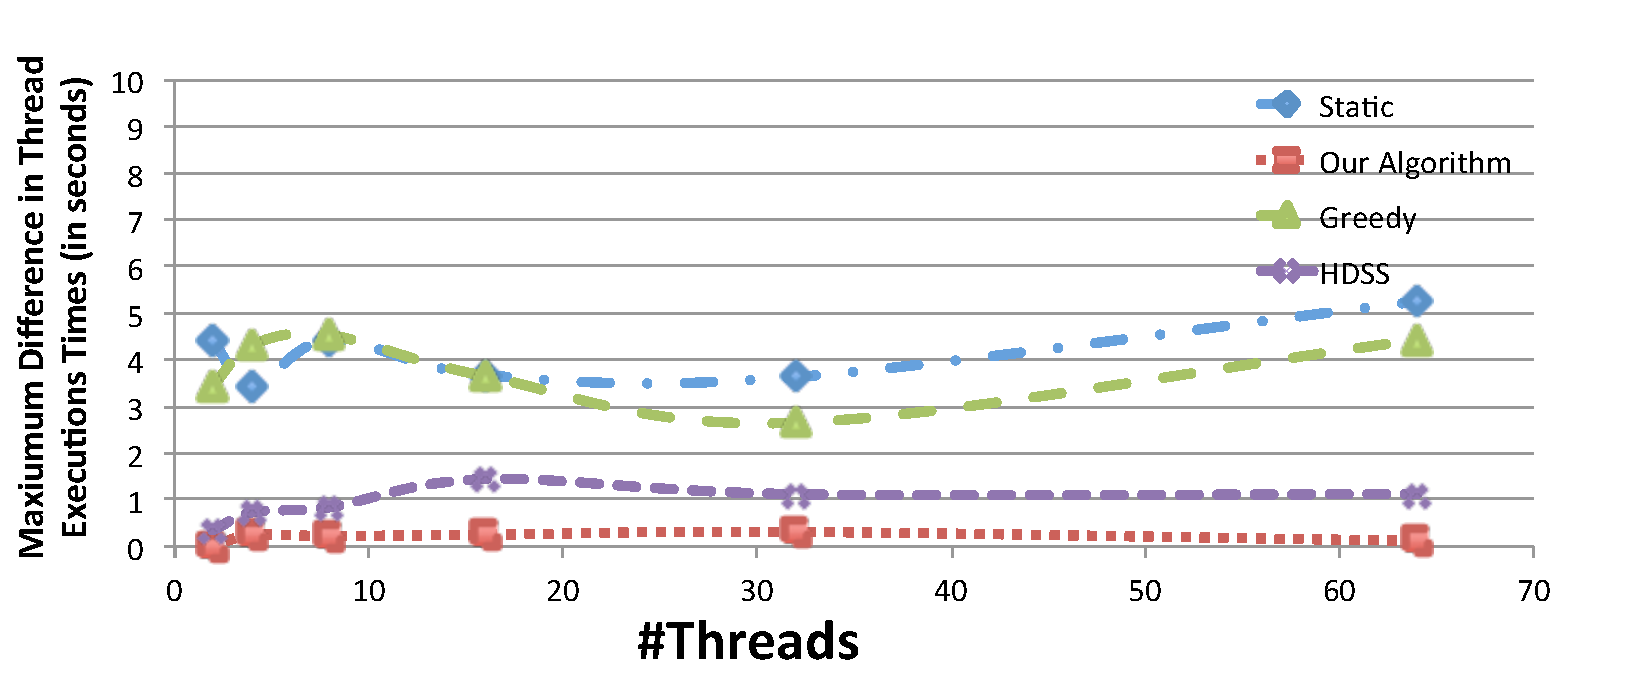
\includegraphics[scale=0.33]{MaximoDiferenca_black_novo.pdf}
%	\caption{Time differences between the earliest and latest finishing threads}
%	\label{fig:diferencaThreadsBlack}
%	\end{center}
%\end{figure}

%Figure~\ref{fig:diferencaThreadsBlack} confirms this result, showing that the
%time difference among the earliest and latest finishing threads in the
%scenario with four machines is always smaller for our proposed algorithm.


%------------------------------------------------------------------------------------------------
\subsection{Gene regulatory networks inference}

We used a third application that performs the inference of Gene Regulatory
Network (GRN) for comparing the four load-balancing algorithms. The results are
shown in Figure~\ref{fig:Gene}. We consider the GRN application with different
number of genes. Our algorithm was configured with a threshold of 10\% of the
execution time and initial block size of 2048 elements. The initial block size
of HDSS algorithm was 1024 elements. As for the other applications, our
algorithm resulted in faster executions, with larger differences with two or
more machines.

\begin{figure*}[htb]
	\begin{center}
	\centering
			%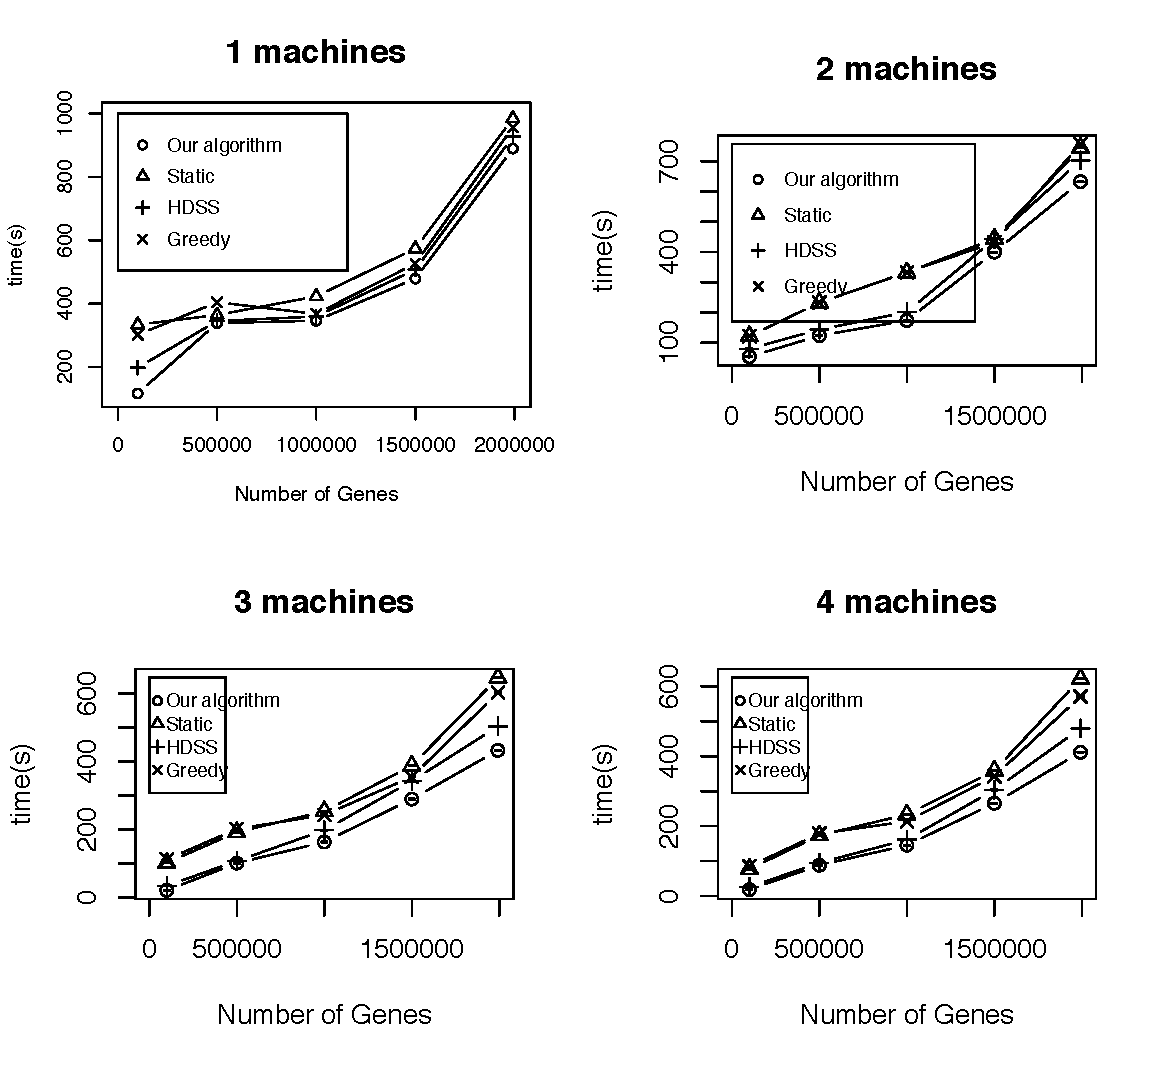
\includegraphics[scale=0.4]{GraficoFabrizio4maquinasNOVO.pdf}
		%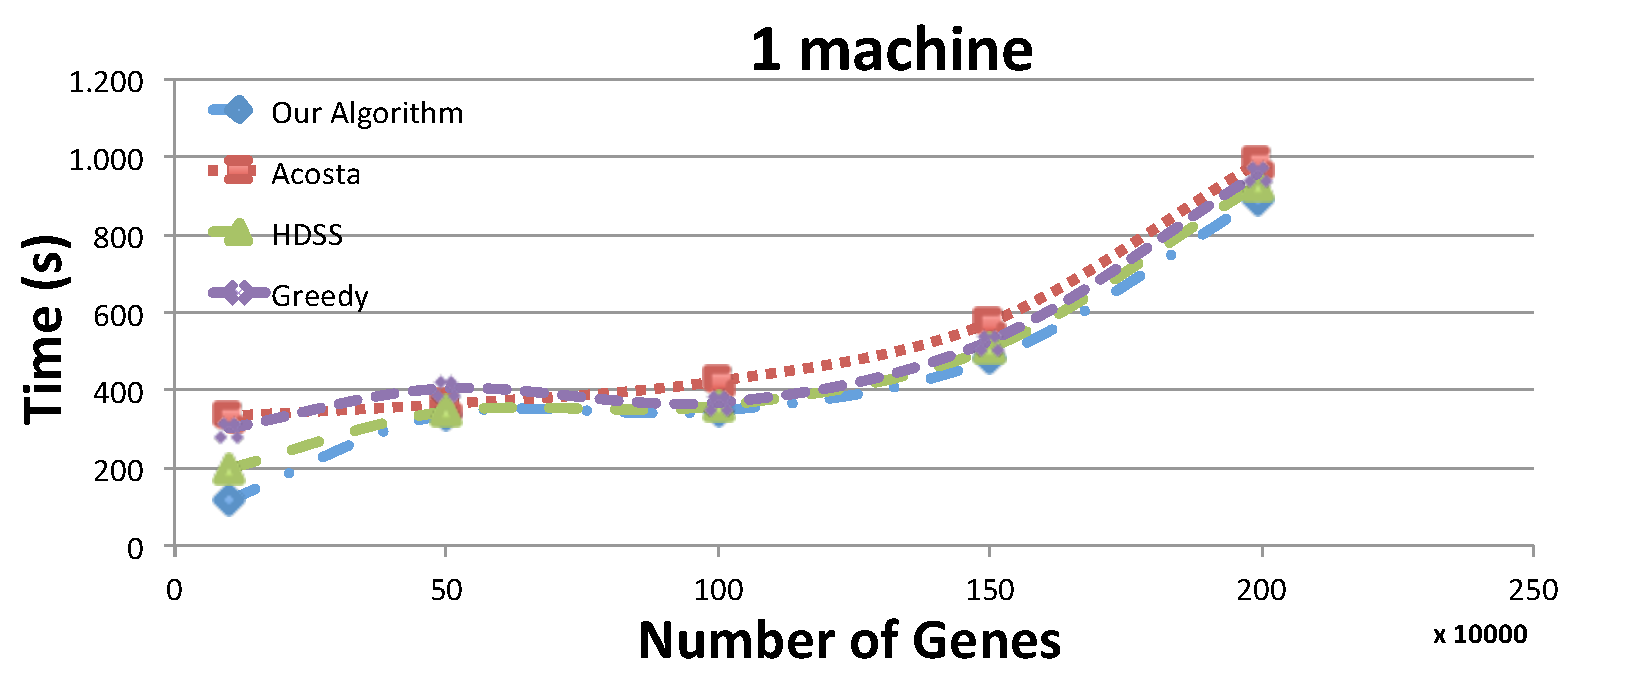
\includegraphics[scale=0.3]{1machineGene.pdf} \quad
		%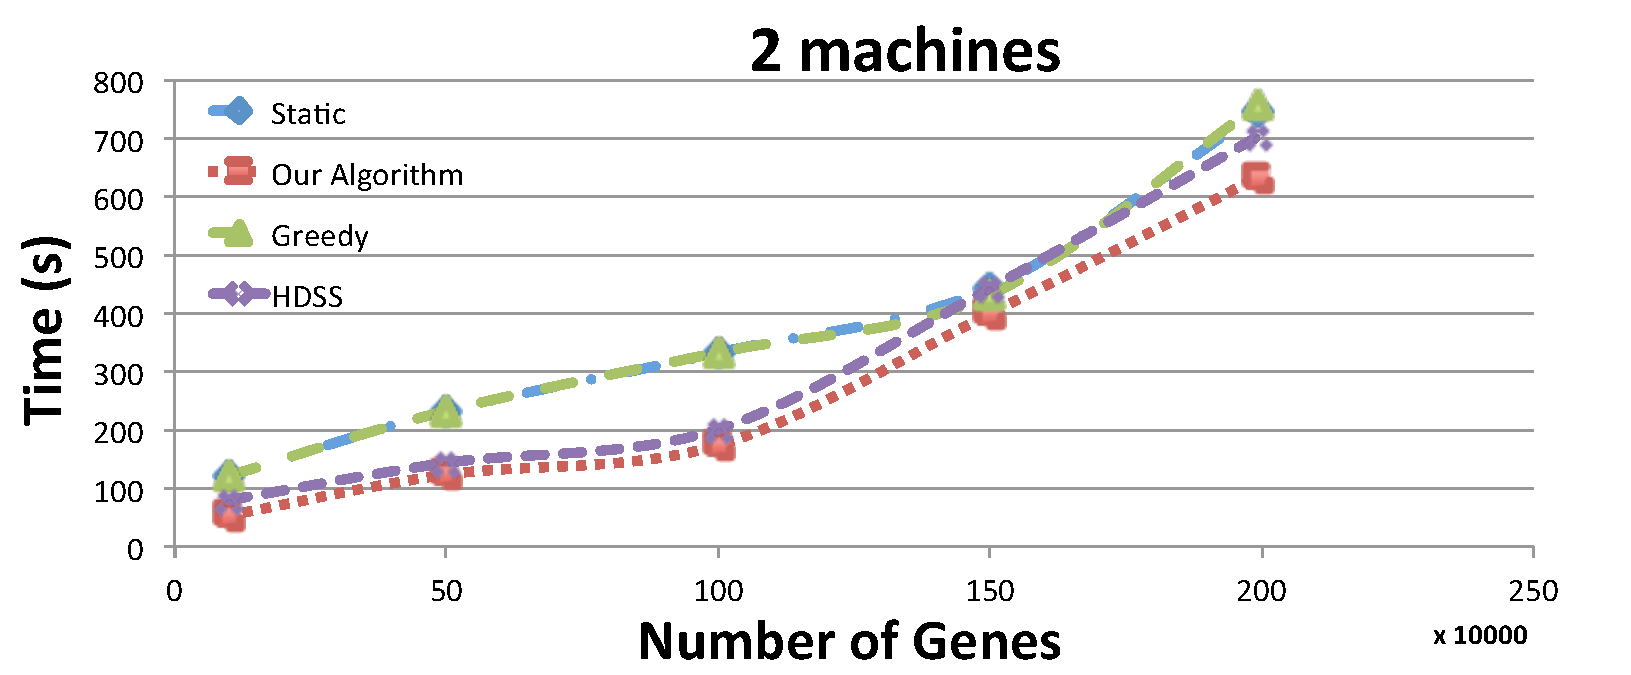
\includegraphics[scale=0.3]{2machineGenes.pdf} \quad
		%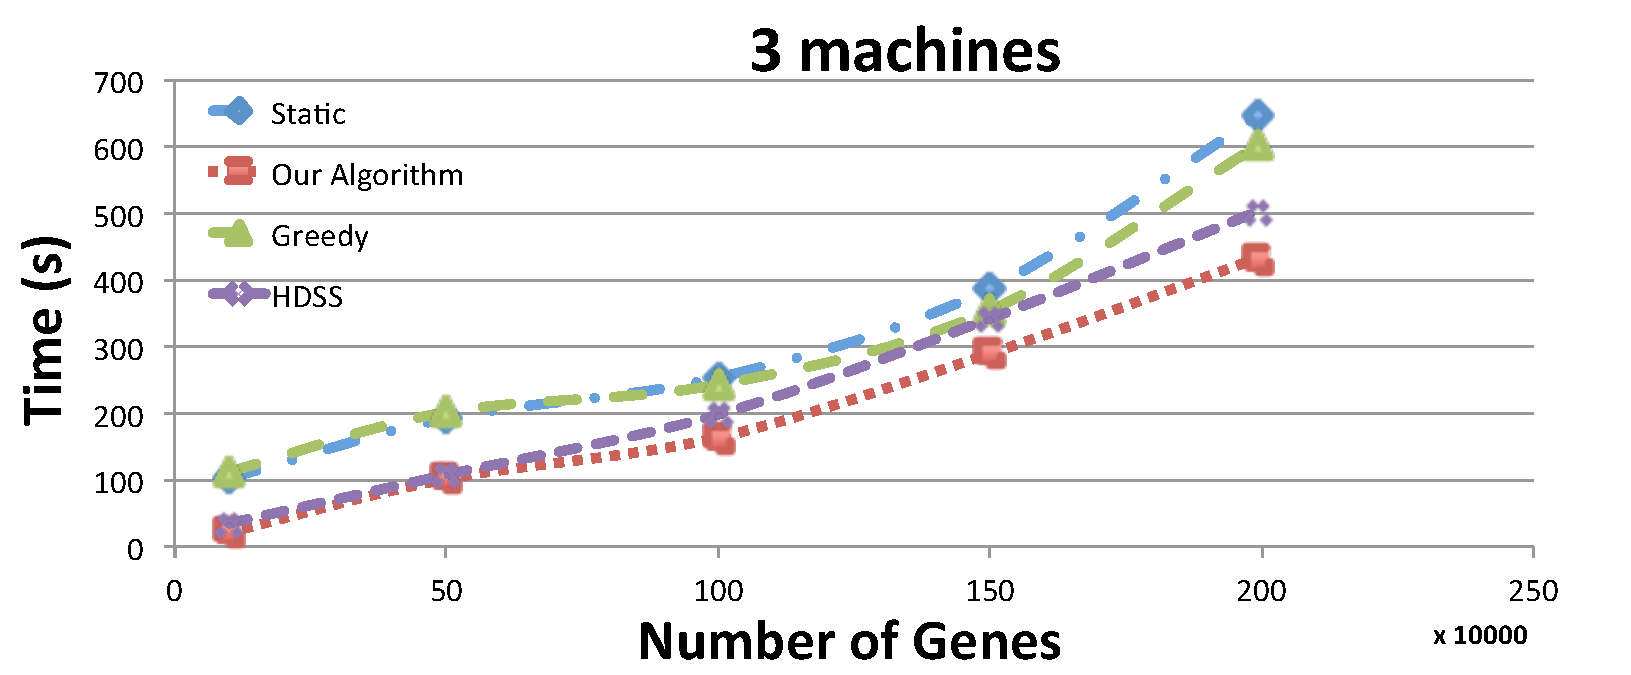
\includegraphics[scale=0.3]{3machineGenes.pdf} \quad
		%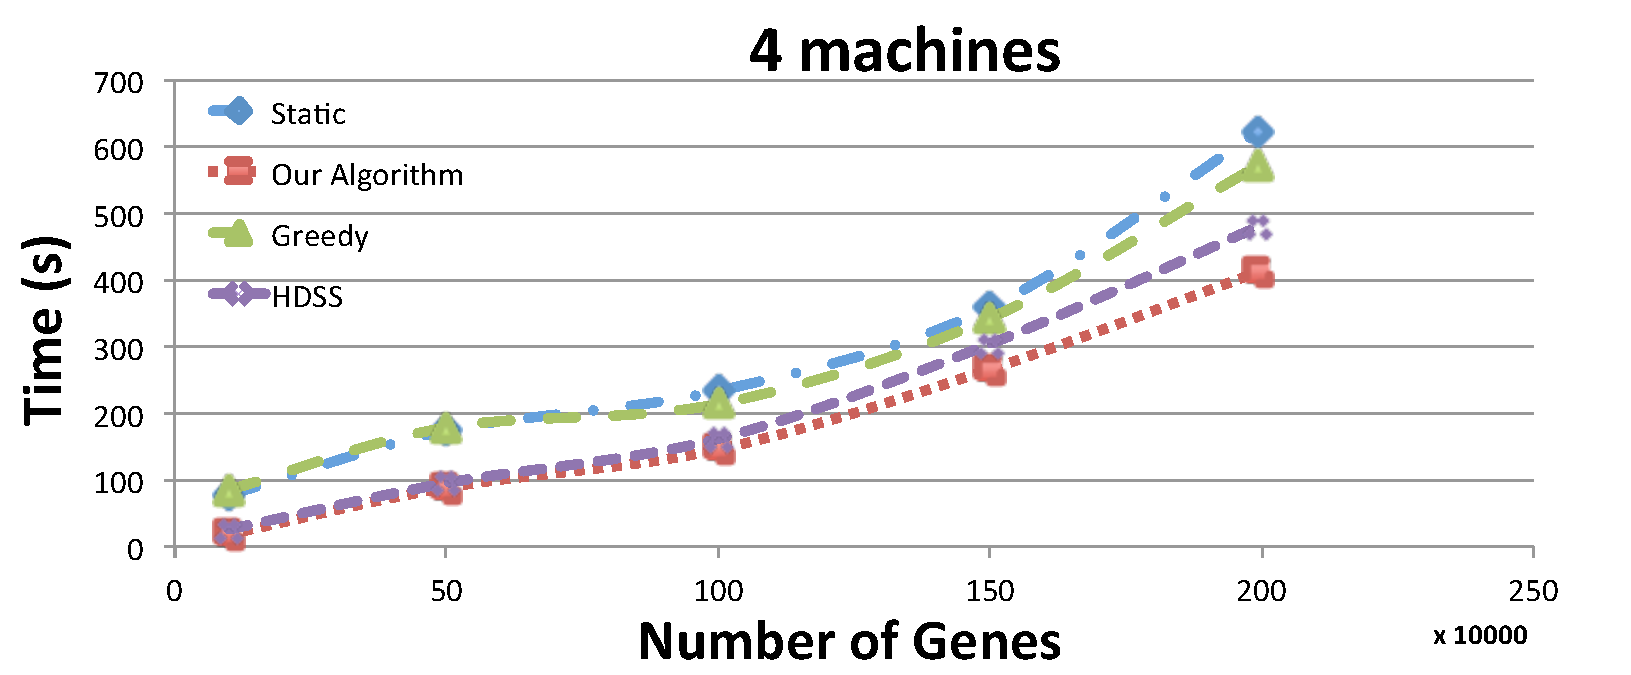
\includegraphics[scale=0.3]{4machineGenes.pdf} 

		\subfigure[1 machine]{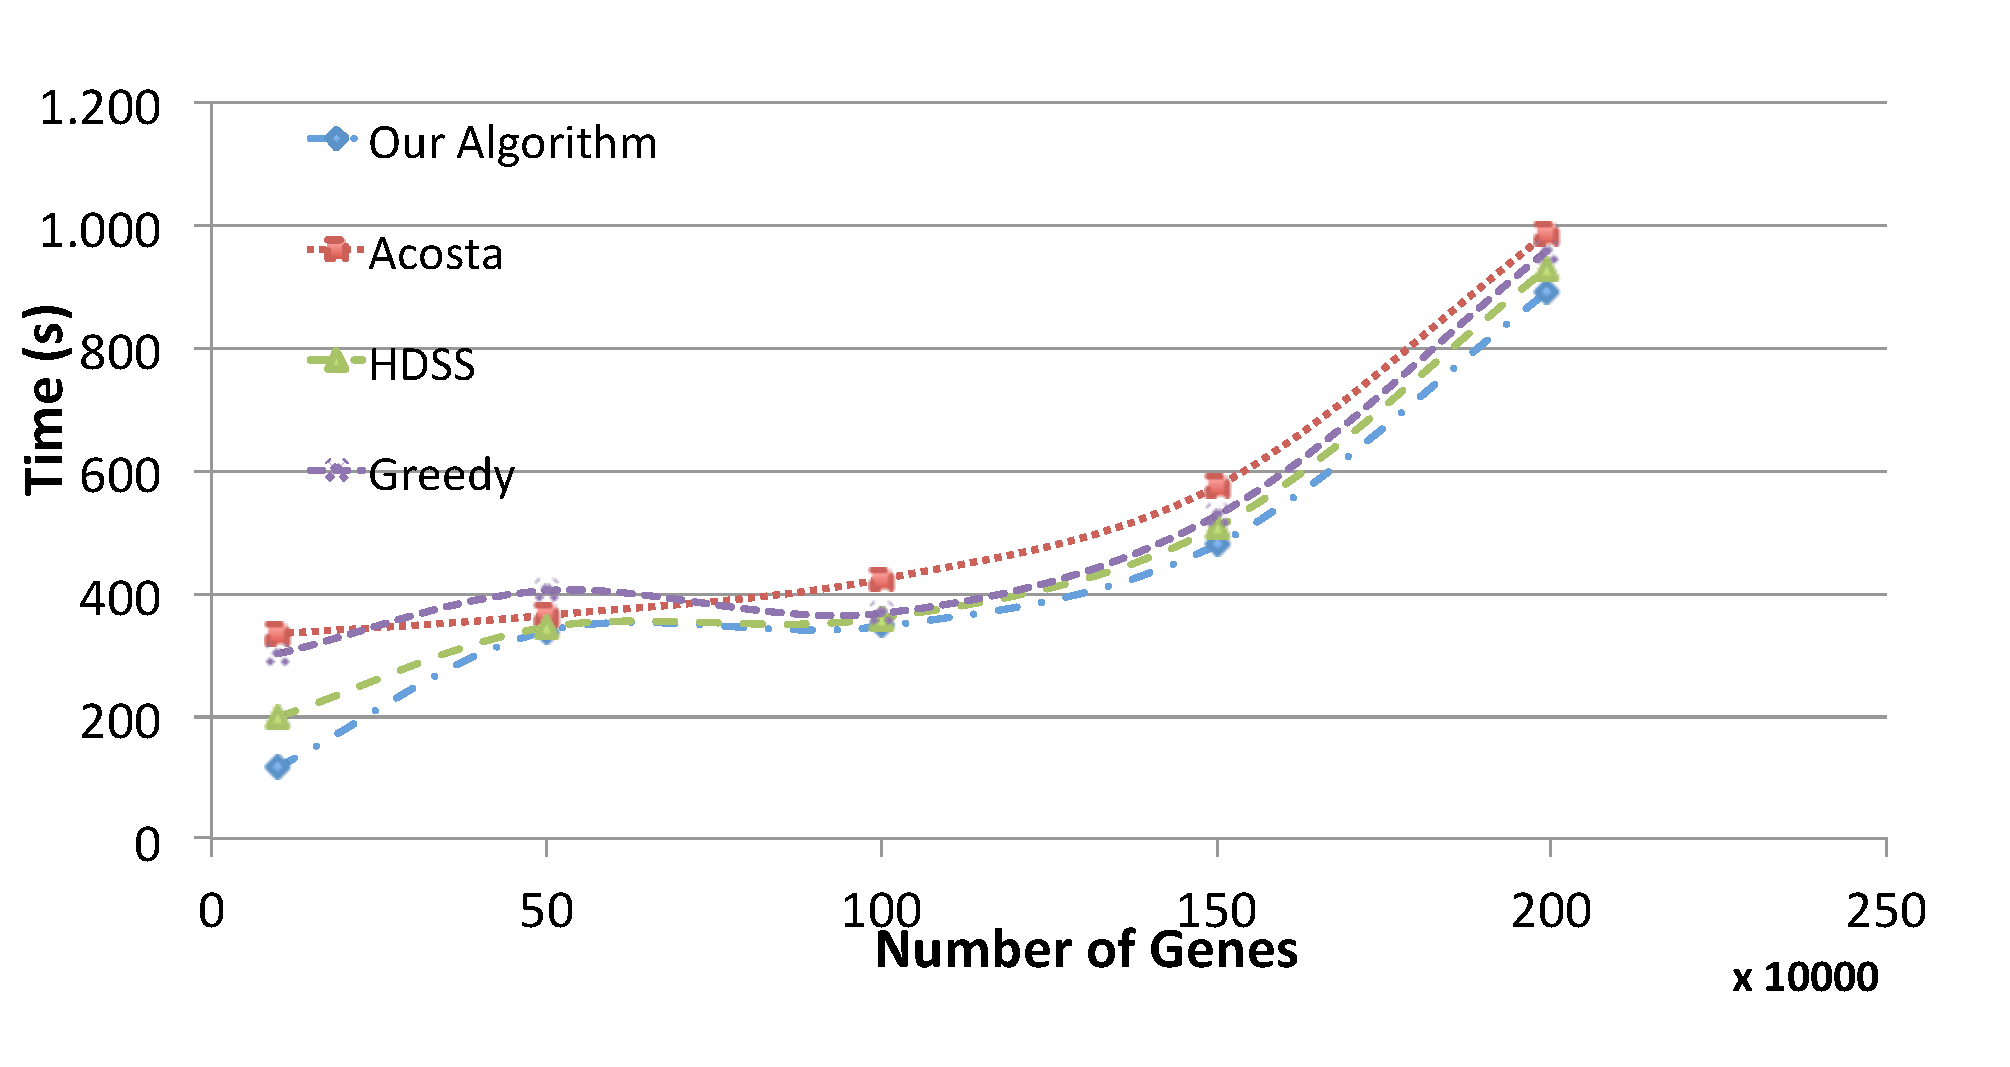
\includegraphics[height=3.3cm, width=4.52cm]{1machineGeneN.pdf}}
	        \subfigure[2 machine]{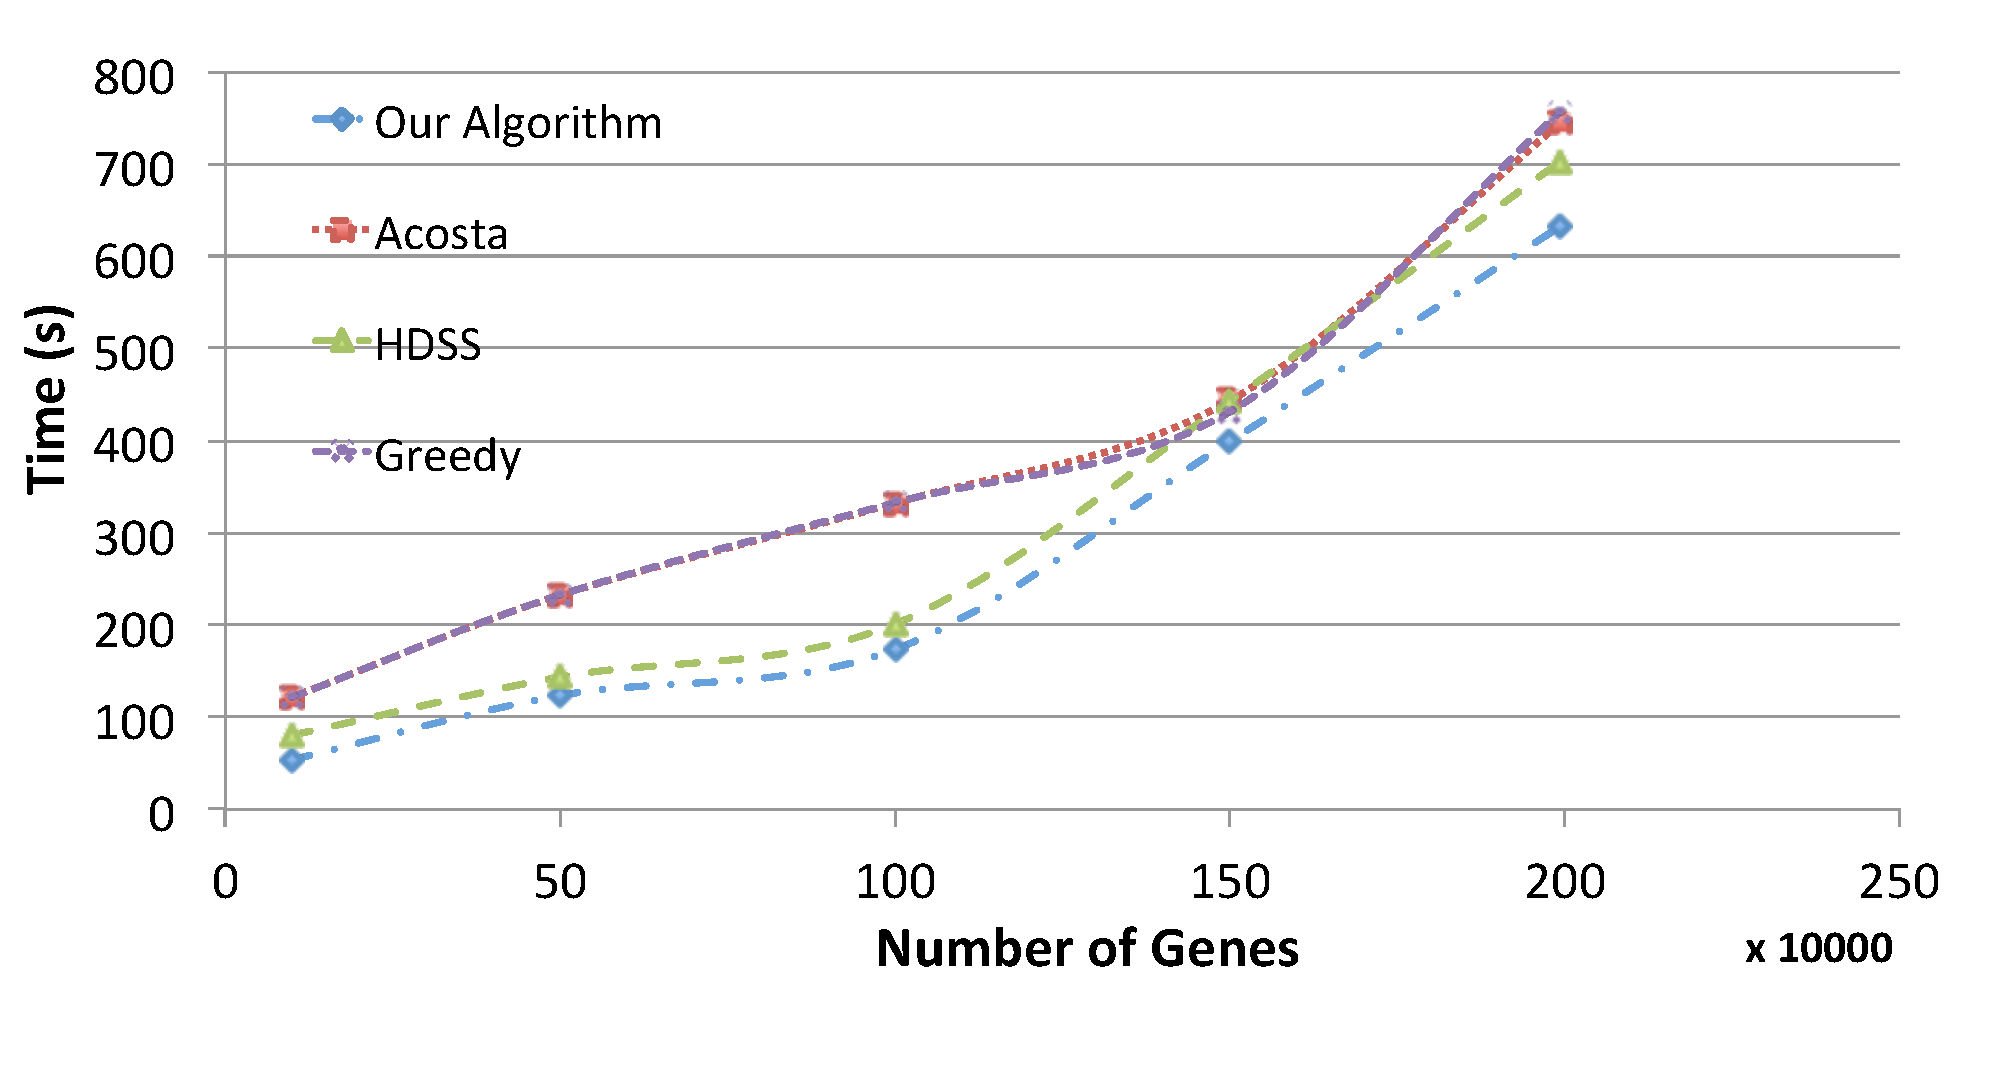
\includegraphics[height=3.3cm, width=4.52cm]{2machineGeneN.pdf}}
		\subfigure[3 machine]{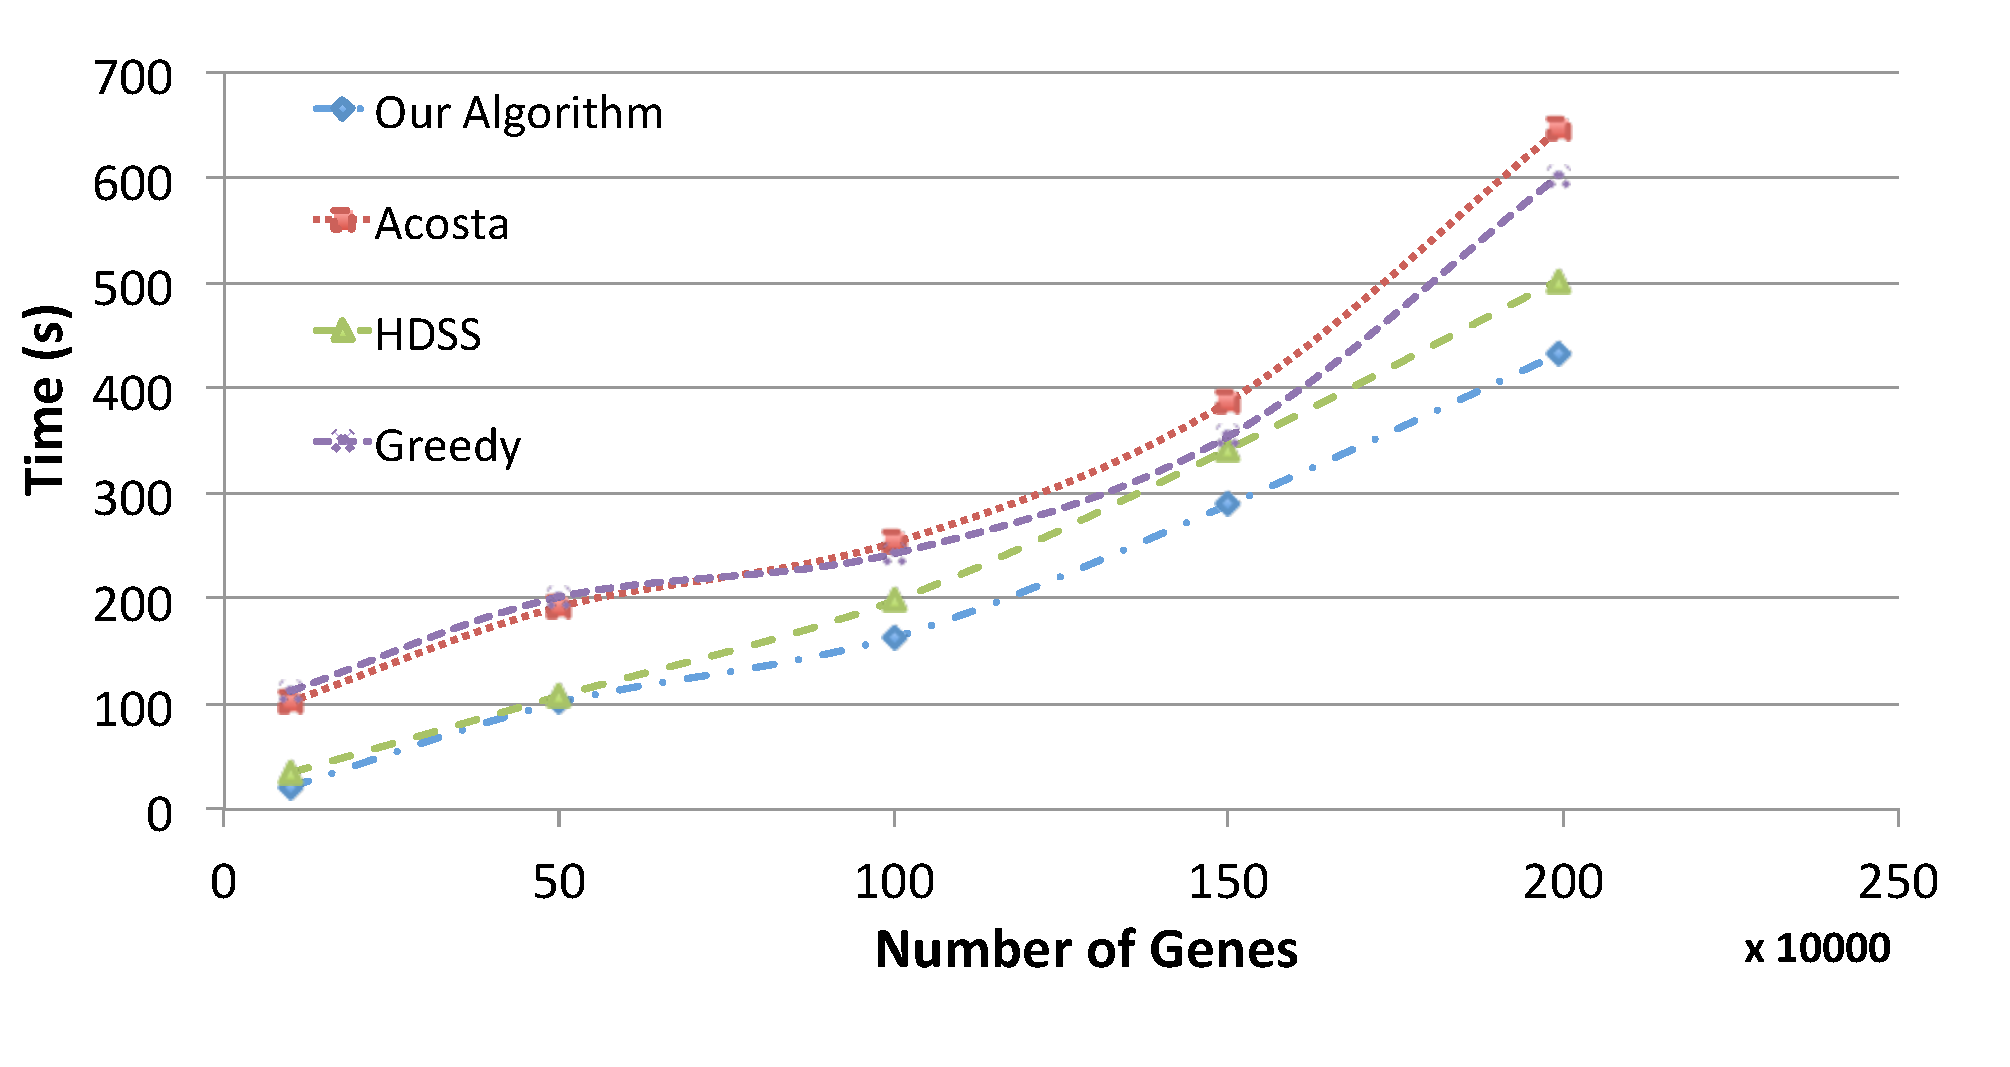
\includegraphics[height=3.3cm, width=4.52cm]{3machineGeneN.pdf}}
		\subfigure[4 machine]{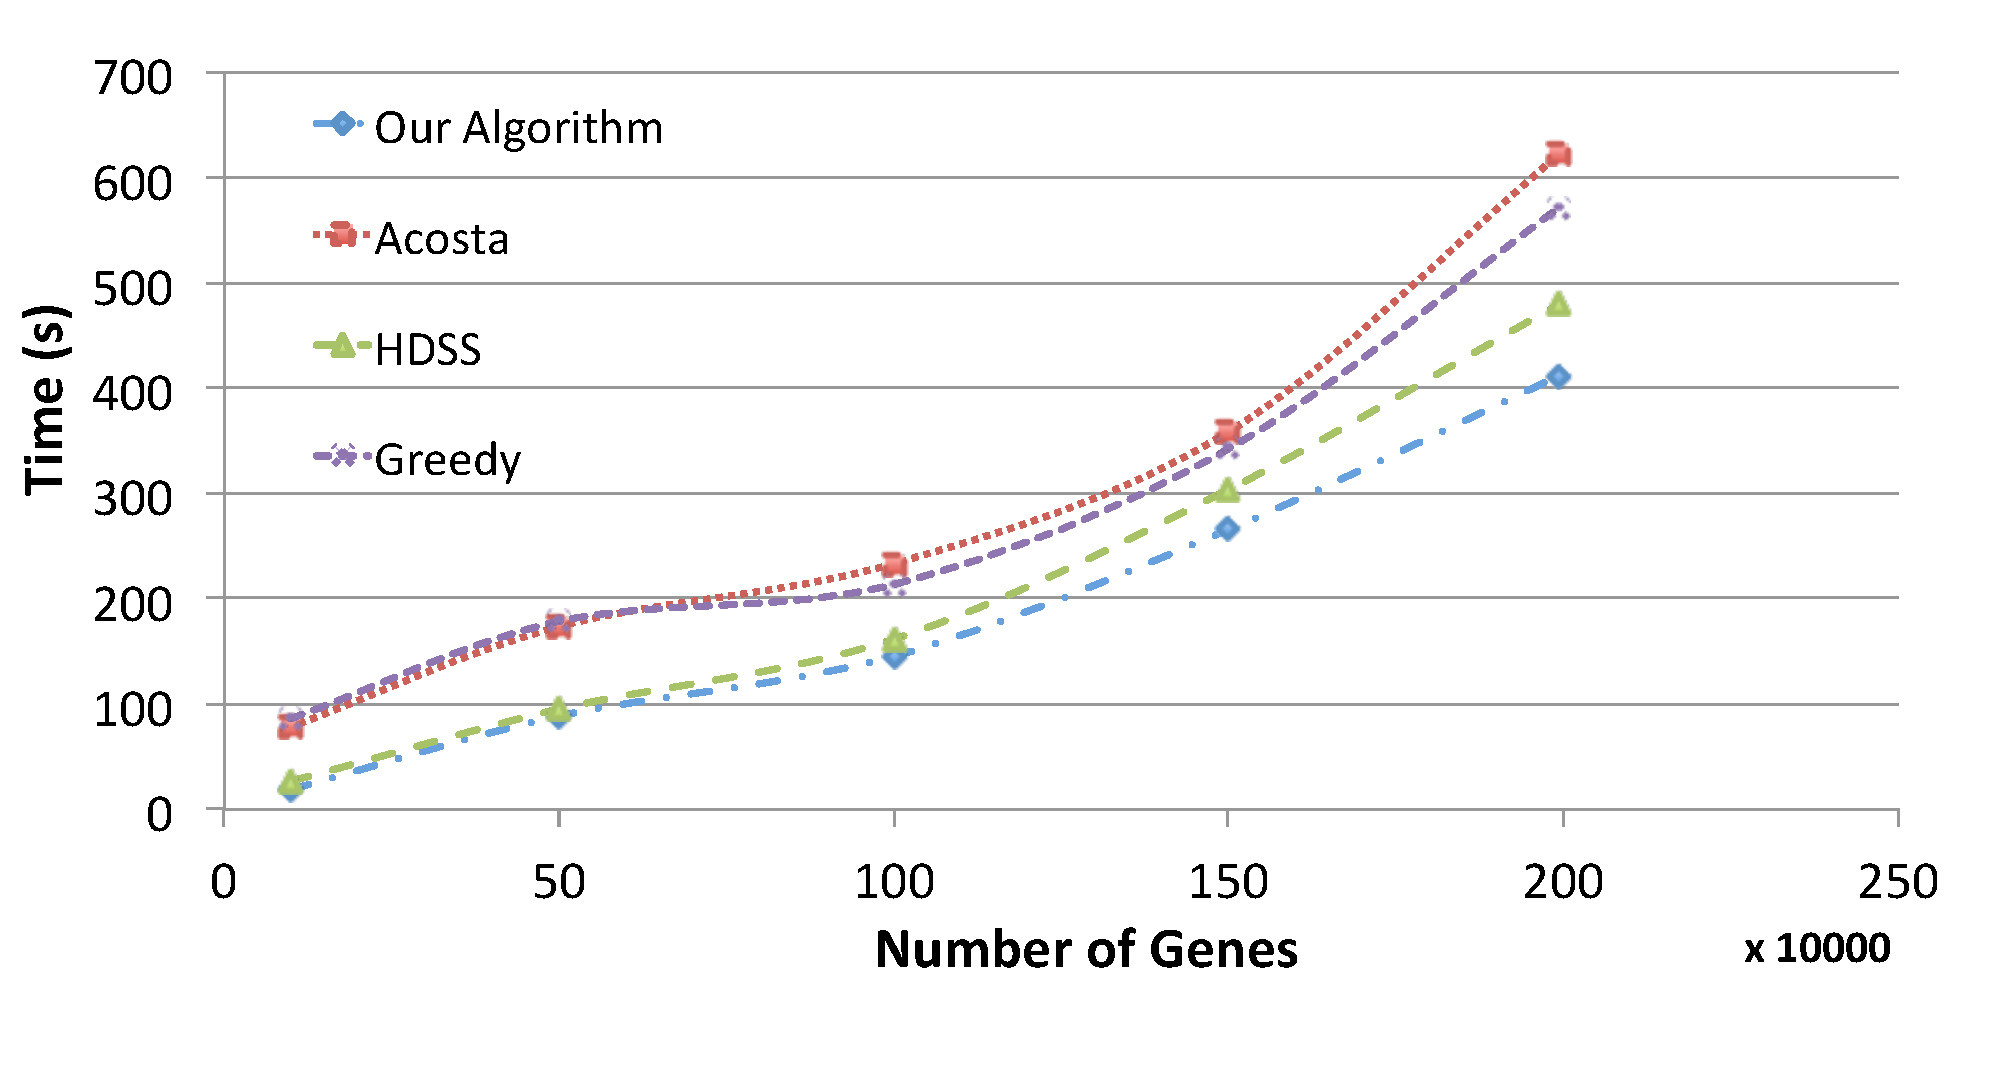
\includegraphics[height=3.3cm, width=4.52cm]{4machineGeneN.pdf}}
	\caption{Difference in runtime with different numbers of genes for gene regulatory network inference}
	\label{fig:Gene}
	\end{center}
\end{figure*}

% RYC: Luís, você consegue explicar por que os ganhos para redes menores são
% maiores? Não está meio estranho? Precisa averiguar o que ocorreu?

%Eu rodei mais de uma vez para analisar os resultados e parece mesmo que para redes menores o ganho é maior. Eu notei que com redes grandes, há muita comunicacao, diferente das redes pequenas, entao se copia da memoria da GPU para CPU os resultados e transfere entre máquinas, algumas vezes para redes grandes. Entao as minhas ideias para o ganho ser maior com redes pequenas é a diminuição de cópias GPU/CPU, menor tráfico na rede e diminuição de sincronizações. Mas precisávamos de mais tempo para ter certeza do motivo.

Table~\ref{table: gene} shows the execution times for 100,000 and 2,000,000
genes using our algorithm and HDSS. In this application, the differences were
larger for the smaller networks. This occurs mainly because on larger networks
the amount of data transfer between machines and in the CPU/GPU interface in
larger networks increases considerably. Since our algorithm do not consider this
communication cost when defining the task sizes, it compromises the
determination of optimal task sizes for the processors.

The total cost of calculating the distribution of the blocks, with four machines
and 2,000,000 genes, using our algorithm was 821.54ms with a standard deviation
of 142.23ms. The overhead was small compared to the application execution time
and was compensated by the better distribution of load.


\begin{table*}[htb]
\centering
\caption{GRN inference application execution times with HDSS and our algorithm}
\begin{scriptsize}
\begin{tabular}{c|c|c|c|c|c|c|}
\cline{2-7}
\multicolumn{1}{l|}{}                 & \multicolumn{3}{c|}{100,000 Genes}                              & \multicolumn{3}{c|}{2,000,000 Genes}                                                  \\ \hline
\multicolumn{1}{|l|}{Num. Machines} & HDSS (s) & Algorithm (s) & \multicolumn{1}{l|}{Diff. (\%)} & \multicolumn{1}{l|}{HDSS (s)} & Algorithm (s) & \multicolumn{1}{l|}{Diff. (\%)} \\ \hline
\multicolumn{1}{|c|}{1 }       &197.94     & 116.43              & 70.00                         & 927.43                         & 889.13              &           4.31                 \\ \hline
\multicolumn{1}{|c|}{2 }      & 79.76     & 53.43              & 49.28                            & 702.65                          & 632.73              & 11.05                           \\ \hline
\multicolumn{1}{|c|}{3 }      & 34.76     & 21.39              & 62.50                            & 502.65                          & 432.43             &               16.24                  \\ \hline
\multicolumn{1}{|c|}{4 }      & 25.91     & 18.54              & 39.75                            & 479.54                          & 411.46             &               16.54  \\ \hline
\end{tabular}
\end{scriptsize}
\label{table: gene}
\end{table*}

\begin{table*}[htb]
\centering
\caption{Distribution of block sizes for GRN inference application}
\begin{scriptsize}
\begin{tabular}{|l|l|l|l|l|l|l|l|}
\cline{3-8}
\multicolumn{1}{l}{} &  & \multicolumn{2}{c|}{Acosta} & \multicolumn{2}{c|}{HDSS} & \multicolumn{2}{c|}{Our Algorithm} \\ 
\cline{3-8}
\multicolumn{1}{l}{} &  & \multicolumn{1}{c|}{100,000 genes} & \multicolumn{1}{c|}{2,000,000 genes} & \multicolumn{1}{c|}{100,000 genes} & \multicolumn{1}{c|}{2,000,000 genes} & \multicolumn{1}{c|}{100,000 genes} & \multicolumn{1}{c|}{2,000,000 genes} \\ 
\cline{1-8}
\multicolumn{1}{|c}{} Machines &  & Size Ratio & Size Ratio & Size Ratio & Size Ratio & Size Ratio & Size Ratio \\ 
\hline
A & CPU & \multicolumn{1}{c|}{$0.08 \pm 0.014$} & \multicolumn{1}{c|}{$0.09 \pm 0.014$} & \multicolumn{1}{c|}{$0.05 \pm 0.018$} & \multicolumn{1}{c|}{$0.06 \pm 0.017$}& \multicolumn{1}{c|}{$0.02 \pm 0.018$} & \multicolumn{1}{c|}{$0.05 \pm 0.018$} \\ 
\cline{2-8}
 & GPU & \multicolumn{1}{c|}{$0.14 \pm 0.014$} & \multicolumn{1}{c|}{$0.11 \pm 0.014$} & \multicolumn{1}{c|}{$0.16 \pm 0.017$} & \multicolumn{1}{c|}{$0.14 \pm 0.018$} & \multicolumn{1}{c|}{$0.08 \pm 0.019$} & \multicolumn{1}{c|}{$0.12 \pm 0.019$} \\ 
\hline
B & CPU & \multicolumn{1}{c|}{$0.06 \pm 0.014$} & \multicolumn{1}{c|}{$0.08 \pm 0.014$} & \multicolumn{1}{c|}{$0.08 \pm 0.018$} & \multicolumn{1}{c|}{$0.06 \pm 0.018$} & \multicolumn{1}{c|}{$0.03 \pm 0.018$} & \multicolumn{1}{c|}{$0.04 \pm 0.018$} \\ 
\cline{2-8}
 & GPU & \multicolumn{1}{c|}{$0.13 \pm 0.014$} & \multicolumn{1}{c|}{$0.14 \pm 0.014$} & \multicolumn{1}{c|}{$0.15 \pm 0.018$} & \multicolumn{1}{c|}{$0.16 \pm 0.017$} & \multicolumn{1}{c|}{$0.12 \pm 0.018$} & \multicolumn{1}{c|}{$0.11 \pm 0.019$} \\ 
\hline
C & CPU & \multicolumn{1}{c|}{$0.11 \pm 0.014$} & \multicolumn{1}{c|}{$0.12 \pm 0.014$} & \multicolumn{1}{c|}{$0.08 \pm 0.018$} & \multicolumn{1}{c|}{$0.05 \pm 0.018$} & \multicolumn{1}{c|}{$0.04 \pm 0.018$} & \multicolumn{1}{c|}{$0.05 \pm 0.018$} \\ 
\cline{2-8}
 & GPU & \multicolumn{1}{c|}{$0.2 \pm 0.014$} & \multicolumn{1}{c|}{$0.19 \pm 0.014$} & \multicolumn{1}{c|}{$0.21 \pm 0.018$} & \multicolumn{1}{c|}{$0.21 \pm 0.018$} & \multicolumn{1}{c|}{$0.34 \pm 0.019$} & \multicolumn{1}{c|}{$0.29 \pm 0.019$} \\ 
\hline
D & CPU & \multicolumn{1}{c|}{$0.07 \pm 0.015$} & \multicolumn{1}{c|}{$0.09 \pm 0.015$} & \multicolumn{1}{c|}{$0.08 \pm 0.019$} & \multicolumn{1}{c|}{$0.08 \pm 0.018$} & \multicolumn{1}{c|}{$0.04 \pm 0.018$} & \multicolumn{1}{c|}{$0.07 \pm 0.018$} \\ 
\cline{2-8}
 & GPU & \multicolumn{1}{c|}{$0.19 \pm 0.015$} & \multicolumn{1}{c|}{$0.17 \pm 0.016$} & \multicolumn{1}{c|}{$0.19 \pm 0.019$} & \multicolumn{1}{c|}{$0.24 \pm 0.018$} & \multicolumn{1}{c|}{$0.33 \pm 0.019$} & \multicolumn{1}{c|}{$0.27 \pm 0.019$} \\ 
\hline
\end{tabular}
\end{scriptsize}
\label{table: comparativoGene}
\end{table*}

Table~\ref{table: comparativoGene} compares the distribution of blocks among the
machines, using 100,000 and 2,000,000 genes and the same experimental setup from
Table~\ref{table: comparativoBlocos}. We observe the same behavior from the
Matrix multiplication application, with Acosta and HDSS algorithms producing
similar distributions while our algorithm distribute proportionally larger
blocks to the GPUs with larger number of cores and smaller blocks to CPUs.


\begin{table*}[htb]
\centering
\caption{Idle processor times for GRN inference application}
\begin{scriptsize}
\begin{tabular}{|l|l|l|l|l|l|}
\cline{3-6}
\multicolumn{1}{l}{} &  & \multicolumn{2}{c|}{HDSS} & \multicolumn{2}{c|}{Our Algorithm} \\ 
\cline{3-6}
\multicolumn{1}{l}{} &  & \multicolumn{1}{c|}{100,000 genes} & \multicolumn{1}{c|}{2,000,000 genes} & \multicolumn{1}{c|}{100,000 genes} & \multicolumn{1}{c|}{2,000,000 genes} \\ 
\cline{1-6}
\multicolumn{1}{|c}{} Machines &  & Idle Time (s) & Idle Time (s) & Idle Time (s) & Idle Time (s) \\ 
\hline
A & CPU & \multicolumn{1}{c|}{$1.2 \pm 0.19$} & \multicolumn{1}{c|}{$9.33 \pm 0.98$} & \multicolumn{1}{c|}{$0.25 \pm 0.06$} & \multicolumn{1}{c|}{$1.36 \pm 0.09$} \\ 
\cline{2-6}
 & GPU & \multicolumn{1}{c|}{$1.4 \pm 0.19$} & \multicolumn{1}{c|}{$7.21 \pm 0.98$} & \multicolumn{1}{c|}{$0.22 \pm 0.07$} & \multicolumn{1}{c|}{$1.67 \pm 0.09$} \\ 
\hline
B & CPU & \multicolumn{1}{c|}{$1.2 \pm 0.19$} & \multicolumn{1}{c|}{$8.98 \pm 0.98$} & \multicolumn{1}{c|}{$0.30 \pm 0.06$} & \multicolumn{1}{c|}{$1.31 \pm 0.09$} \\ 
\cline{2-6}
 & GPU & \multicolumn{1}{c|}{$0.8 \pm 0.19$} & \multicolumn{1}{c|}{$7.39 \pm 0.98$} & \multicolumn{1}{c|}{$0.29 \pm 0.06$} & \multicolumn{1}{c|}{$1.45 \pm 0.09$} \\ 
\hline
C & CPU & \multicolumn{1}{c|}{$1.2 \pm 0.19$} & \multicolumn{1}{c|}{$9.21 \pm 0.98$} & \multicolumn{1}{c|}{$0.23 \pm 0.08$} & \multicolumn{1}{c|}{$1.21 \pm 0.09$} \\ 
\cline{2-6}
 & GPU & \multicolumn{1}{c|}{$0.9 \pm 0.18$} & \multicolumn{1}{c|}{$9.32 \pm 0.98$} & \multicolumn{1}{c|}{$0.28 \pm 0.06$} & \multicolumn{1}{c|}{$1.64 \pm 0.09$} \\ 
\hline
D & CPU & \multicolumn{1}{c|}{$1.3 \pm 0.19$} & \multicolumn{1}{c|}{$9.92 \pm 0.98$} & \multicolumn{1}{c|}{$0.27 \pm 0.08$} & \multicolumn{1}{c|}{$1.22 \pm 0.09$} \\ 
\cline{2-6}
 & GPU & \multicolumn{1}{c|}{$1.1 \pm 0.19$} & \multicolumn{1}{c|}{$9.97 \pm 0.99$} & \multicolumn{1}{c|}{$0.21 \pm 0.06$} & \multicolumn{1}{c|}{$1.55 \pm 0.1$} \\ 
\hline
\end{tabular}
\end{scriptsize}
\label{table: ociosidadeGene}
\end{table*}

Finally, Table~\ref{table: ociosidadeGene} presents the time each processor from
each machine was idle using the HDSS and our algorithm with 100,000 and
2,000,000 genes. The idleness periods were significantly superior using the HDSS
algorithm, which is in accordance with the large difference in the execution time of
the GRN application using both algorithms. This application has an execution
time which has a cubical increase in execution time in relation to the block
size. In this case, unbalanced block distributions cause a larger impact in the
execution time.

%When analyzing the differences with thread finishing time, shown in
%Figure~\ref{fig:GeneDiferenca}, we see that again our algorithm has the smalles
%differences, due to its more precise task size definition procedure.

%\begin{figure}[htb]
%	\begin{center}
%	\centering
%			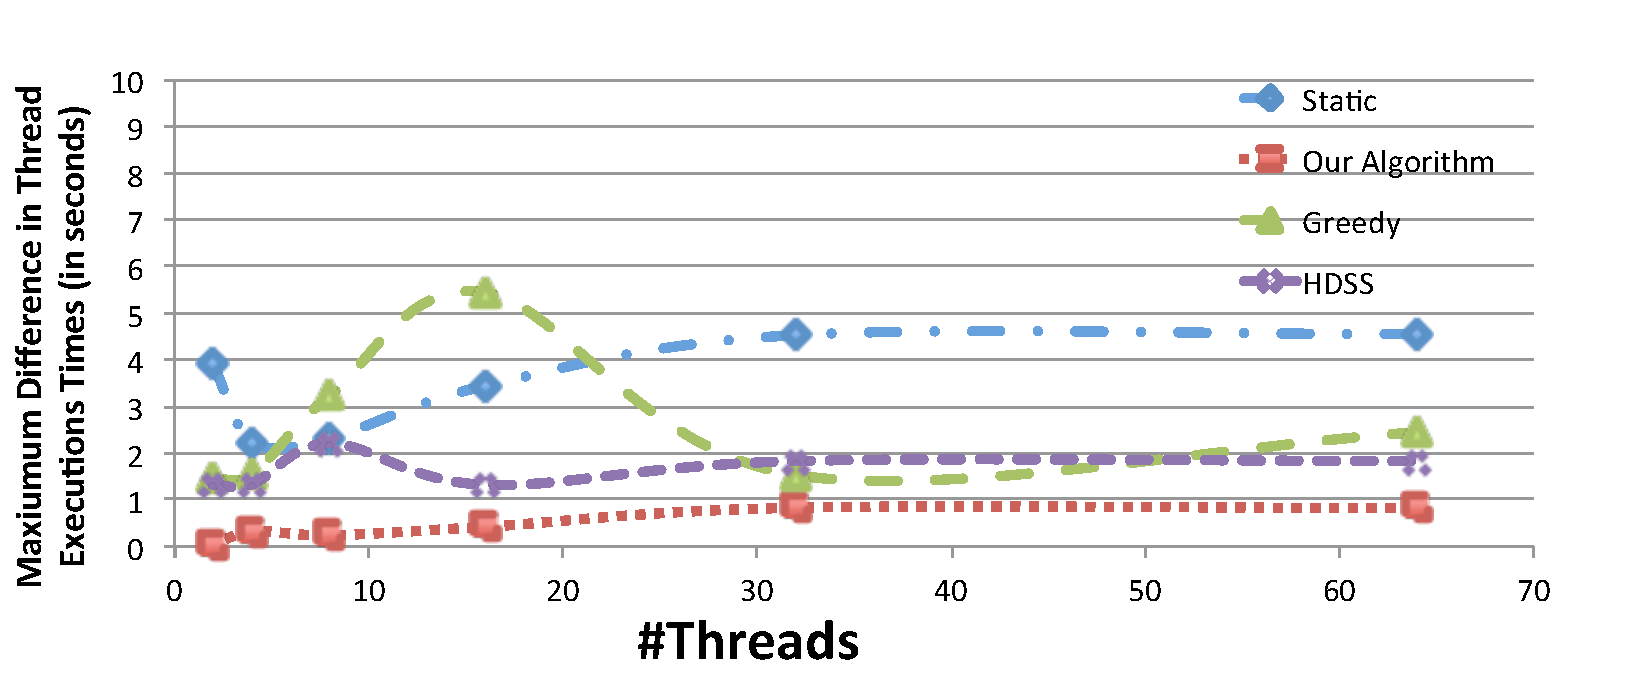
\includegraphics[scale=0.33]{MaximoDiferenca_fabrizio_novo.pdf}
%	\caption{Time differences between the earliest and latest finishing threads for GRN}
%	\label{fig:GeneDiferenca}
%	\end{center}
%\end{figure}

%--------------------------------------------------------------------------
%\subsection{Block size evolution}

%We also evaluated the effect of changing the environment conditions during the application execution using our algorithm and HDSS. We used the GRN inference application and three machines (A, B and C). In this example, the three machines were concurrently running a graphical application on the GPU, which was cancelled on machine C 400s the start of the execution of the GRN application. This simulates a scenario where the user has no exclusive access to the cluster, as is commom in shared clusters.

%The topmost graph in Figure~\ref{fig:GeneBlocos} shows the block sizes generated
%by our algorithm.  We can see that the algorithm initially finds, after the processor performance modeling phase, a distribution of blocks that favors machine C. In a later moment, before 400s, the concurrent application that was executing on machine C finishes. Our algorithm detects that the difference in the task
%finishing times was above the defined threshold. In this case, it triggered a
%rebalancing process of tasks sizes, which are maintained until the end of the
%execution. 

% RYC: Por que é vantajoso para o HDSS diminuir o tamanho das tarefas? Explicar no texto, Ok.
%In HDSS the the block sizes decrease during the execution until the last
%iteration, for all units complete execution at nearly the same time. This
%prevents that unbalances in the final of the execution cause some processors to
%receive large portions data while other remains idle. This decrease in block
%size reduces length of this idleness period. But the proportion of block sizes
%allocated to different processors is maintained, resulting that a sub-optimal
%distribution of block sizes is maintained during the entire execution.

% RYC: Usar machine A, B and C nas figuras, para ficar de acordo com as
% descrições das máquinas. ->OK

%\begin{figure}[htb]
%	\begin{center}
%	\centering
%			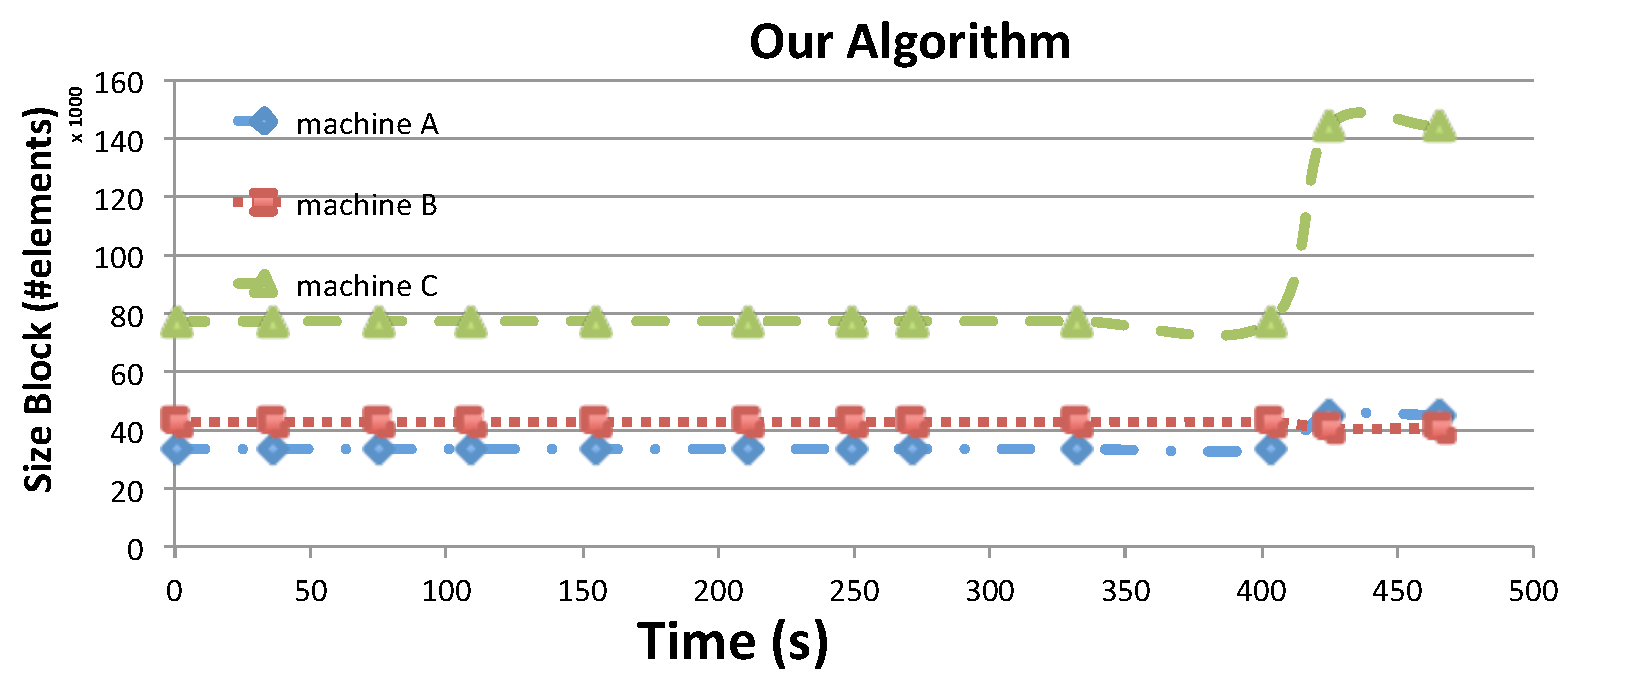
\includegraphics[scale=0.33]{Block_Comportamento_Nosso.pdf}%\quad
%			%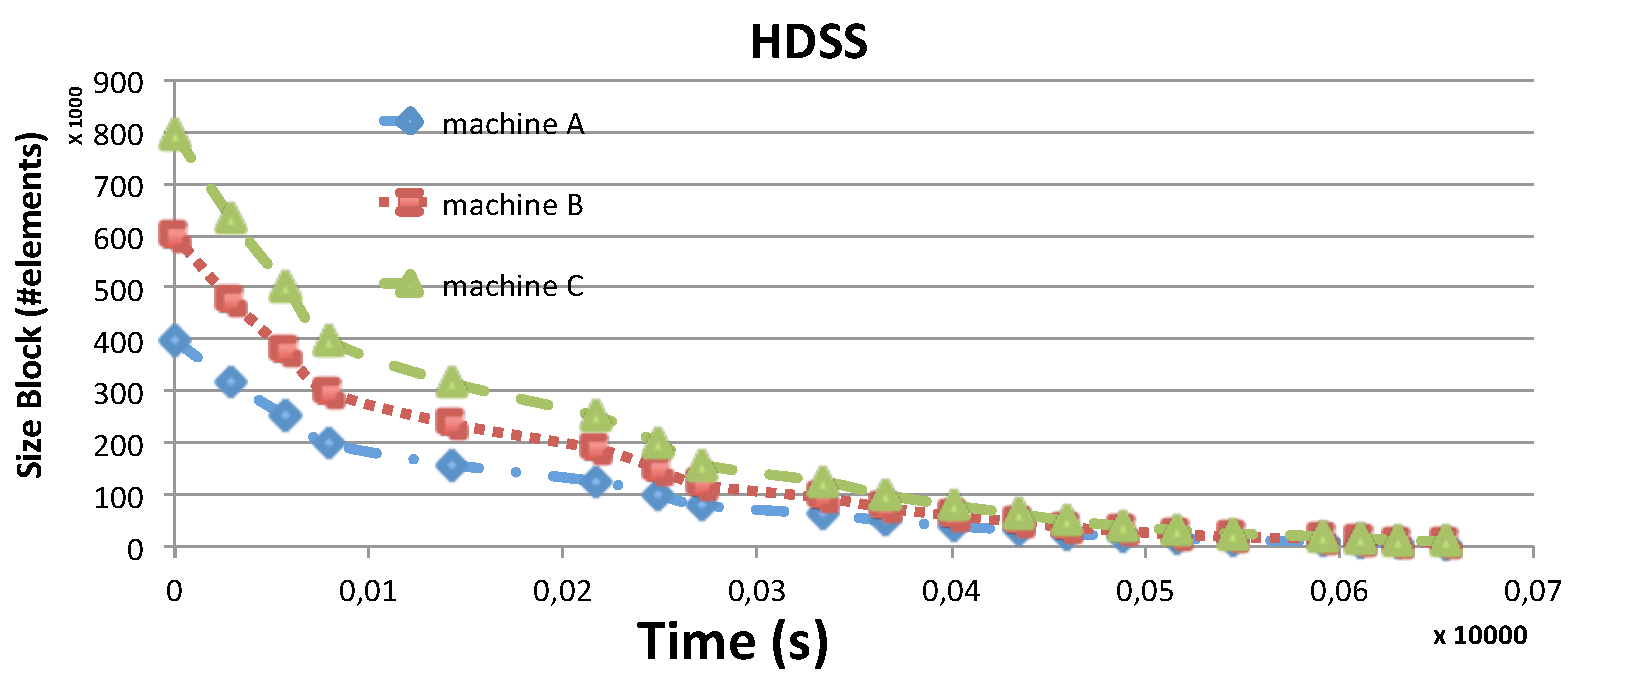
\includegraphics[scale=0.33]{Block_Comportamento_Deles.pdf}
%	\caption{Block size evolution for GRN application.}
%	\label{fig:GeneBlocos}
%	\end{center}
%\end{figure}


%-------------------------------------------------------------------------------
\section{Conclusions and future work}

In this paper we propose a load-balancing algorithm for distributing tasks among
processors in domain decomposition problems executing on clusters of
heterogeneous CPUs and GPUs. It outperforms other similar existing algorithms,
due to the online estimation of performance curve models for each processing
unit and the selection of the best data distribution for the processors using an
interior point method for solving a non-linear system of equations. We evaluated
the algorithms using three types of applications and our load-balancing
algorithm reduced the execution times in all scenarios, with the largest
improvements in more heterogeneous environments.

Although we used dedicated clusters in the experiments, we can also consider the
usage of public clouds or non-dedicated shared machines. In these scenarios, the
quality of service may change during execution, reducing or increasing the
amount computational hardware allocated to the application. The usage of a
re-balancing threshold in our algorithm permits permits readjustments in data
distributions. But it is necessary to evaluate under what conditions our
algorithm can successfully compensate this change in the environment. We could
also consider the scenario with added fault-tolerance, where machines may become
unavailable during execution. If the application is fault-tolerant, a
re-balancing of the load among the remaining devices would permit the
application to execute efficiently on these devices.

Our next step is to include the cost of communication in the load-balancing
algorithm, which will improve the load-balancing for applications where the time
spent with information exchange between processors is substantial.

% use section* for acknowledgement
\section*{Acknowledgment}

The authors would like to thank UFABC and FAPESP (Proc. n. 2012/03778-0 and
Proc. n.  2013/26644-1) for the financial support and Fabrizio Borelli for
providing the gene regulatory network application.

\ifCLASSOPTIONcaptionsoff
  \newpage
\fi

% trigger a \newpage just before the given reference
% number - used to balance the columns on the last page
% adjust value as needed - may need to be readjusted if
% the document is modified later
%\IEEEtriggeratref{20}  % REAJUSTAR DEPOIS DE TODAS AS MODIFICACOES!
% The "triggered" command can be changed if desired:
%\IEEEtriggercmd{\enlargethispage{-5in}}

% can use a bibliography generated by BibTeX as a .bbl file
% BibTeX documentation can be easily obtained at:
% http://www.ctan.org/tex-archive/biblio/bibtex/contrib/doc/
% The IEEEtran BibTeX style support page is at:
% http://www.michaelshell.org/tex/ieeetran/bibtex/
\bibliographystyle{IEEEtran}
% argument is your BibTeX string definitions and bibliography database(s)
%\bibliography{IEEEabrv,../bib/paper}
%
% <OR> manually copy in the resultant .bbl file
% set second argument of \begin to the number of references
% (used to reserve space for the reference number labels box)
% File .bib
\bibliography{article}


\end{document}


